%%%%%%%%%%%%%%%%%%%%%%%%%%%%%%%%%%%%%%%%%%%%%%%%%%%%%%%%%%%%%%%
%% OXFORD THESIS TEMPLATE

% Use this template to produce a standard thesis that meets the Oxford University requirements for DPhil submission
%
% Originally by Keith A. Gillow (gillow@maths.ox.ac.uk), 1997
% Modified by Sam Evans (sam@samuelevansresearch.org), 2007
% Modified by John McManigle (john@oxfordechoes.com), 2015
%
% This version Copyright (c) 2015-2017 John McManigle
%
% Broad permissions are granted to use, modify, and distribute this software
% as specified in the MIT License included in this distribution's LICENSE file.
%

% I've (John) tried to comment this file extensively, so read through it to see how to use the various options.  Remember
% that in LaTeX, any line starting with a % is NOT executed.  Several places below, you have a choice of which line to use
% out of multiple options (eg draft vs final, for PDF vs for binding, etc.)  When you pick one, add a % to the beginning of
% the lines you don't want.


%%%%% CHOOSE PAGE LAYOUT
% The most common choices should be below.  You can also do other things, like replacing "a4paper" with "letterpaper", etc.

% This one will format for two-sided binding (ie left and right pages have mirror margins; blank pages inserted where needed):
\listfiles
%\documentclass[a4paper,twoside]{ociamthesis}
% This one will format for one-sided binding (ie left margin > right margin; no extra blank pages):
%\documentclass[a4paper]{ociamthesis}
% This one will format for PDF output (ie equal margins, no extra blank pages):
\documentclass[a4paper,nobind]{ociamthesis} 



%%%%% SELECT YOUR DRAFT OPTIONS
% Three options going on here; use in any combination.  But remember to turn the first two off before
% generating a PDF to send to the printer!

% This adds a "DRAFT" footer to every normal page.  (The first page of each chapter is not a "normal" page.)
\fancyfoot[C]{\emph{DRAFT Printed on \today}}  

% This highlights (in blue) corrections marked with (for words) \mccorrect{blah} or (for whole
% paragraphs) \begin{mccorrection} . . . \end{mccorrection}.  This can be useful for sending a PDF of
% your corrected thesis to your examiners for review.  Turn it off, and the blue disappears.
\correctionstrue


%%%%% BIBLIOGRAPHY SETUP
% Note that your bibliography will require some tweaking depending on your department, preferred format, etc.
% The options included below are just very basic "sciencey" and "humanitiesey" options to get started.
% If you've not used LaTeX before, I recommend reading a little about biblatex/biber and getting started with it.
% If you're already a LaTeX pro and are used to natbib or something, modify as necessary.
% Either way, you'll have to choose and configure an appropriate bibliography format...

% The science-type option: numerical in-text citation with references in order of appearance.
\usepackage[style=numeric-comp, sorting=none, backend=biber, doi=false, isbn=false]{biblatex}
\usepackage{glossaries}
\usepackage{fancyvrb}
\usepackage[textsize=tiny]{todonotes}
\presetkeys{todonotes}{inline}{}
\usepackage{listings}
\usepackage{xcolor}
%\usepackage{glossaries-extra}
\newcommand*{\bibtitle}{References}
\usepackage{hyperref}
\usepackage{cleveref} 

\usepackage{booktabs}
\usepackage{longtable}
\usepackage{array}
\usepackage{multirow}
\usepackage{wrapfig}
\usepackage{float}
\usepackage{colortbl}
\usepackage{pdflscape}
\usepackage{tabu}
\usepackage{threeparttable}
\usepackage{threeparttablex}
\usepackage[normalem]{ulem}
\usepackage{makecell}
\usepackage{xcolor}
\usepackage{tabularx}

\makenoidxglossaries

\newacronym{smc2}{SMCSMC}{Sequential Monte Carlo for the Sequentially Markovian Coalescent}

\newacronym{ooa}{OoA}{Out of Africa}
\newacronym{kya}{kya}{kiloanni (thousands of years) before present}
\newacronym{amh}{AMH}{anatomically modern human}
\newacronym{sgdp}{SGDP}{Simons Genome Diversity Panel}
\newacronym{hgdp}{HGDP}{Human Genome Diversity Panel}
\newacronym{ngs}{NGS}{Next Generation Sequencing}
\newacronym{ibd}{IBD}{Identity by Descent}
\newacronym{tmrca}{TMRCA}{Time to Most Recent Common Ancestor}
\newacronym{mtDNA}{mtDNA}{Mitochondrial DNA}
\newacronym{arg}{ARG}{Ancestral Recombination Graph}
\newacronym{cahg}{CAHG}{Central African Hunter Gatherer}
\newacronym{sahg}{SAHG}{South African Hunter Gatherer}
\newacronym{imf}{IMF}{Integrated Migration Fraction}
\newacronym[sort=ne]{ne}{$N_e$}{Effective Population Size}
\newglossaryentry{msmc}{
    name = MSMC,
    description = {Multiply Sequentially Markovian Coalescent. A program developed in \cite{Schiffels2014}.}
}
\newglossaryentry{msmc2}{
    name = MSMC2,
    description = {Multiply Sequentially Markovian Coalescent, version 2. This updated version has not yet been published.} 
}

\newglossaryentry{scrm}{
    name = SCRM,
    description = {Both a method and its implementation for the sequential coalescent with recombination.}
}


\newacronym{ebv}{EBV}{Epstein-Barr Virus}
\newacronym{lda}{LDA}{Latent Dirichlet Allocation}
\newacronym{ohe}{OHE}{One-hot Encoding}

\newacronym{tfbs}{TFBS}{Transcription factor binding site}
\newacronym{pwm}{PWM}{Position weight matrix}
\newacronym{dna}{DNA}{deoxyribonucleic acid}
\newacronym{rna}{RNA}{ribonucleic acid}
\newacronym{cre}{CRE}{cis-regulatory element}
\newacronym{hsc}{HSC}{hematopoietic stem cell}
\newacronym{atac}{ATAC-seq}{Assay of Transposase Accessible Chromatin sequencing}
\newacronym{tf}{TF}{Transcription factor}
\newacronym{scatac}{scATAC-seq}{Single cell ATAC-seq}
\newacronym{mcmc}{MCMC}{Markov chain Monte Carlo}
\newacronym{bcp}{BCP}{B-cell precursor}
\newacronym{all}{ALL}{acute lymphoblastic leukemia}
\newacronym{lnc}{lncRNA}{long non-coding RNA}
\newacronym{chip}{ChIP-seq}{Chromatin immunoprecipitation followed by sequencing}
\newacronym{mll}{KMT2A}{lysine methyltransferase 2A}
\newacronym{aml}{AML}{acute myeloid leukemia}
\newacronym{lsc}{LSC}{leukemia stem cell}
\newacronym{ukbb}{UKBB}{United Kingdom BioBank}
\newacronym{blda}{BLDA}{bulk latent dirichlet allocation}
\newacronym{wgs}{WGS}{whole genome sequencing}
\newacronym{fp}{KMT2A-FP}{KMT2A fusion protein}

\newacronym{srs}{SRS}{short-read sequencing}
\newacronym{lrs}{LRS}{long-read sequencing}
\newacronym{sbs}{SBS}{sequencing by synthesis}
\newacronym{sbl}{SBL}{sequencing by ligation}
\newacronym{indel}{InDel}{insertion or deletion}
\newacronym{mrca}{MRCA}{most recent common ancestor}
\newacronym{ld}{LD}{linkage disequilibrium}
\newacronym{cwr}{CwR}{coalescent with recombination}
\newacronym{smc}{SMC}{sequentially Markovian coalescent}
\newacronym{psmc}{PSMC}{pairwise sequentially Markovian coalescent}
\newacronym{iicr}{IICR}{inverse instantaneous coalescence rate}
\newacronym{sfs}{SFS}{site frequency spectrum}
\newacronym{hmm}{HMM}{hidden Markov model}
\newacronym{pcr}{PCR}{polymerase chain reaction}
\newacronym{snp}{SNP}{single nucleotide polymorphism}
\newacronym{tss}{TSS}{transcription start site}
\newacronym{dot1l}{DOT1L}{ disruptor of telomeric silencing 1-like}
%\setacronymstyle{}{long-short}
\setcounter{secnumdepth}{3}
\setcounter{tocdepth}{3}


\definecolor{codegreen}{rgb}{0,0.6,0}
\definecolor{codegray}{rgb}{0.5,0.5,0.5}
\definecolor{codepurple}{rgb}{0.58,0,0.82}
\definecolor{backcolour}{rgb}{0.95,0.95,0.92}

\lstdefinestyle{mystyle}{
    backgroundcolor=\color{backcolour},   
    commentstyle=\color{codegreen},
    keywordstyle=\color{magenta},
    numberstyle=\tiny\color{codegray},
    stringstyle=\color{codepurple},
    basicstyle=\ttfamily\footnotesize,
    breakatwhitespace=false,         
    breaklines=true,                 
    captionpos=b,                    
    keepspaces=true,                 
    numbers=left,                    
    numbersep=5pt,                  
    showspaces=false,                
    showstringspaces=false,
    showtabs=false,                  
    tabsize=2
}

\lstset{style=mystyle}


% The humanities-type option: author-year in-text citation with an alphabetical works cited.
%\usepackage[style=authoryear, sorting=nyt, backend=biber, maxcitenames=2, useprefix, doi=false, isbn=false]{biblatex}
%\newcommand*{\bibtitle}{Works Cited}

% This makes the bibliography left-aligned (not 'justified') and slightly smaller font.
\renewcommand*{\bibfont}{\raggedright\small}

% Change this to the name of your .bib file (usually exported from a citation manager like Zotero or EndNote).
\addbibresource{references.bib}
\addbibresource{bib/thesis.bib}


% Uncomment this if you want equation numbers per section (2.3.12), instead of per chapter (2.18):
%\numberwithin{equation}{subsection}



%%%%% THESIS / TITLE PAGE INFORMATION
% Everybody needs to complete the following:
%\title{Machine learning for genetic variation: applications to leukemia and demographic inference}
\title{Machine learning methods for the interpretation of next generation sequencing data: applications to leukemia and demographic inference}
\author{Christopher B. Cole}
\college{Exeter College}

% Master's candidates who require the alternate title page (with candidate number and word count)
% must also un-comment and complete the following three lines:
%\masterssubmissiontrue
%\candidateno{933516}
%\wordcount{28,815}

% Uncomment the following line if your degree also includes exams (eg most masters):
%\renewcommand{\submittedtext}{Submitted in partial completion of the}
% Your full degree name.  (But remember that DPhils aren't "in" anything.  They're just DPhils.)
\degree{Doctor of Philosophy}
% Term and year of submission, or date if your board requires (eg most masters)
\degreedate{Michaelmas 2021}


%%%%% YOUR OWN PERSONAL MACROS
% This is a good place to dump your own LaTeX macros as they come up.

% To make text superscripts shortcuts
%\renewcommand{\th}{\textsuperscript{th}} % ex: I won 4\th place
%\newcommand{\nd}{\textsuperscript{nd}}
%\renewcommand{\st}{\textsuperscript{st}}
%\newcommand{\rd}{\textsuperscript{rd}}

%%%%% THE ACTUAL DOCUMENT STARTS HERE
\begin{document}



%%%%% CHOOSE YOUR LINE SPACING HERE
% This is the official option.  Use it for your submission copy and library copy:
\setlength{\textbaselineskip}{22pt plus2pt}
% This is closer spacing (about 1.5-spaced) that you might prefer for your personal copies:
%\setlength{\textbaselineskip}{18pt plus2pt minus1pt}

% You can set the spacing here for the roman-numbered pages (acknowledgements, table of contents, etc.)
\setlength{\frontmatterbaselineskip}{17pt plus1pt minus1pt}

% Leave this line alone; it gets things started for the real document.
\setlength{\baselineskip}{\textbaselineskip}


%%%%% CHOOSE YOUR SECTION NUMBERING DEPTH HERE
% You have two choices.  First, how far down are sections numbered?  (Below that, they're named but
% don't get numbers.)  Second, what level of section appears in the table of contents?  These don't have
% to match: you can have numbered sections that don't show up in the ToC, or unnumbered sections that
% do.  Throughout, 0 = chapter; 1 = section; 2 = subsection; 3 = subsubsection, 4 = paragraph...

% The level that gets a number:
\setcounter{secnumdepth}{3}
% The level that shows up in the ToC:
\setcounter{tocdepth}{3}
\setcounter{minitocdepth}{3}


%%%%% ABSTRACT SEPARATE
% This is used to create the separate, one-page abstract that you are required to hand into the Exam
% Schools.  You can comment it out to generate a PDF for printing or whatnot.
\begin{abstractseparate}
	As next generation sequencing technologies continue to mature and find applications across genomics, it has become clear that the scale and scope of generated data far exceeds our ability for manual interpretation. Machine learning has shown remarkable success in finding patterns in this data and generating biologically testable hypotheses. In this thesis, I develop and apply machine learning methods which use NGS data to answer outstanding questions in population and functional genomics.

%to infer directional migration from whole genome sequencing (WGS) data and identify shared and distinct regulatory programs in closely related cell types from chromatin accessibility assays. 
An understanding of the genetic history of global populations has been hindered by a lack of methods capable of inferring directional migration over time. 
%Understanding the genetic history of global populations has been a longstanding goal in population genomics, however there has never been a method capable of inferring directional migration over time.
I use a sequential Monte Carlo approach (a particle filter) to sample from the posterior distribution of ancestral recombination graphs and infer likely population size and migration histories from whole genome sequencing data.
%introduce a particle filter for demographic inference which uses a flexible sequential Monte Carlo sampler alongside variational Bayes to determine likely population size and migration histories from whole genome sequencing data. 
I apply this particle filter to global sequencing biobanks and uncover an abundance of migration from the ancestors of non-Africans into Africa between 40 and 70 thousand years ago. I show that latent directional migration has broader implications for the inference of population size in gold-standard approaches and explore this migration in the context of African pre-history.

On a cellular rather than population scale, I apply latent Dirichlet allocation to NGS-based chromatin accessibility assays in order to model shared and distinct regulatory pathways between different cell types. I demonstrate the method's utility by recovering known regulatory biology in erythroblast development. I apply this topic modelling approach to understand cis-regulatory element usage in a treatment-resistant leukemia caused by the MLL-AF4 oncoprotein. The results highlight a previously uncharacterized class of enhancer elements depleted in DOT1L-deposited H3 lysine 79 methylation and enriched for PAF1c binding. 

In this thesis, I have developed and applied machine learning approaches to identify patterns in large genomics databases and answer biological questions on both population and cellular levels.  % Create an abstract.tex file in the 'text' folder for your abstract.
\end{abstractseparate}


% JEM: Pages are roman numbered from here, though page numbers are invisible until ToC.  This is in
% keeping with most typesetting conventions.
\begin{romanpages}

% Title page is created here
\maketitle

%%%%% DEDICATION -- If you'd like one, un-comment the following.
%\begin{dedication}
%This thesis is dedicated to\\
%someone\\
%for some special reason\\
%\end{dedication}

%%%%% ACKNOWLEDGEMENTS -- Nothing to do here except comment out if you don't want it.
\begin{acknowledgements}
 	\subsection*{Personal}

To do.

\subsection*{Institutional}

To do.

\end{acknowledgements}

%%%%% ABSTRACT -- Nothing to do here except comment out if you don't want it.
\begin{abstract}
	As next generation sequencing technologies continue to mature and find applications across genomics, it has become clear that the scale and scope of generated data far exceeds our ability for manual interpretation. Machine learning has shown remarkable success in finding patterns in this data and generating biologically testable hypotheses. In this thesis, I develop and apply machine learning methods which use NGS data to answer outstanding questions in population and functional genomics.

%to infer directional migration from whole genome sequencing (WGS) data and identify shared and distinct regulatory programs in closely related cell types from chromatin accessibility assays. 
An understanding of the genetic history of global populations has been hindered by a lack of methods capable of inferring directional migration over time. 
%Understanding the genetic history of global populations has been a longstanding goal in population genomics, however there has never been a method capable of inferring directional migration over time.
I use a sequential Monte Carlo approach (a particle filter) to sample from the posterior distribution of ancestral recombination graphs and infer likely population size and migration histories from whole genome sequencing data.
%introduce a particle filter for demographic inference which uses a flexible sequential Monte Carlo sampler alongside variational Bayes to determine likely population size and migration histories from whole genome sequencing data. 
I apply this particle filter to global sequencing biobanks and uncover an abundance of migration from the ancestors of non-Africans into Africa between 40 and 70 thousand years ago. I show that latent directional migration has broader implications for the inference of population size in gold-standard approaches and explore this migration in the context of African pre-history.

On a cellular rather than population scale, I apply latent Dirichlet allocation to NGS-based chromatin accessibility assays in order to model shared and distinct regulatory pathways between different cell types. I demonstrate the method's utility by recovering known regulatory biology in erythroblast development. I apply this topic modelling approach to understand cis-regulatory element usage in a treatment-resistant leukemia caused by the MLL-AF4 oncoprotein. The results highlight a previously uncharacterized class of enhancer elements depleted in DOT1L-deposited H3 lysine 79 methylation and enriched for PAF1c binding. 

In this thesis, I have developed and applied machine learning approaches to identify patterns in large genomics databases and answer biological questions on both population and cellular levels. 
\end{abstract}

%%%%% MINI TABLES
% This lays the groundwork for per-chapter, mini tables of contents.  Comment the following line
% (and remove \minitoc from the chapter files) if you don't want this.  Un-comment either of the
% next two lines if you want a per-chapter list of figures or tables.
\dominitoc % include a mini table of contents
%\dominilof  % include a mini list of figures
%\dominilot  % include a mini list of tables

% This aligns the bottom of the text of each page.  It generally makes things look better.
\flushbottom

% This is where the whole-document ToC appears:
\tableofcontents

\listoffigures
\mtcaddchapter
%\mtcaddchapter is needed when adding a non-chapter (but chapter-like) entity to avoid confusing minitoc

% Uncomment to generate a list of tables:
\listoftables
\mtcaddchapter

%\adjustmtc


\printnoidxglossaries

\listoftodos


%%%%% LIST OF ABBREVIATIONS
% This example includes a list of abbreviations.  Look at text/abbreviations.tex to see how that file is
% formatted.  The template can handle any kind of list though, so this might be a good place for a
% glossary, etc.
%\makenoidxglossaries

\newacronym{smc2}{SMCSMC}{Sequential Monte Carlo for the Sequentially Markovian Coalescent}

\newacronym{ooa}{OoA}{Out of Africa}
\newacronym{kya}{kya}{kiloanni (thousands of years) before present}
\newacronym{amh}{AMH}{anatomically modern human}
\newacronym{sgdp}{SGDP}{Simons Genome Diversity Panel}
\newacronym{hgdp}{HGDP}{Human Genome Diversity Panel}
\newacronym{ngs}{NGS}{Next Generation Sequencing}
\newacronym{ibd}{IBD}{Identity by Descent}
\newacronym{tmrca}{TMRCA}{Time to Most Recent Common Ancestor}
\newacronym{mtDNA}{mtDNA}{Mitochondrial DNA}
\newacronym{arg}{ARG}{Ancestral Recombination Graph}
\newacronym{cahg}{CAHG}{Central African Hunter Gatherer}
\newacronym{sahg}{SAHG}{South African Hunter Gatherer}
\newacronym{imf}{IMF}{Integrated Migration Fraction}
\newacronym[sort=ne]{ne}{$N_e$}{Effective Population Size}
\newglossaryentry{msmc}{
    name = MSMC,
    description = {Multiply Sequentially Markovian Coalescent. A program developed in \cite{Schiffels2014}.}
}
\newglossaryentry{msmc2}{
    name = MSMC2,
    description = {Multiply Sequentially Markovian Coalescent, version 2. This updated version has not yet been published.} 
}

\newglossaryentry{scrm}{
    name = SCRM,
    description = {Both a method and its implementation for the sequential coalescent with recombination.}
}


\newacronym{ebv}{EBV}{Epstein-Barr Virus}
\newacronym{lda}{LDA}{Latent Dirichlet Allocation}
\newacronym{ohe}{OHE}{One-hot Encoding}

\newacronym{tfbs}{TFBS}{Transcription factor binding site}
\newacronym{pwm}{PWM}{Position weight matrix}
\newacronym{dna}{DNA}{deoxyribonucleic acid}
\newacronym{rna}{RNA}{ribonucleic acid}
\newacronym{cre}{CRE}{cis-regulatory element}
\newacronym{hsc}{HSC}{hematopoietic stem cell}
\newacronym{atac}{ATAC-seq}{Assay of Transposase Accessible Chromatin sequencing}
\newacronym{tf}{TF}{Transcription factor}
\newacronym{scatac}{scATAC-seq}{Single cell ATAC-seq}
\newacronym{mcmc}{MCMC}{Markov chain Monte Carlo}
\newacronym{bcp}{BCP}{B-cell precursor}
\newacronym{all}{ALL}{acute lymphoblastic leukemia}
\newacronym{lnc}{lncRNA}{long non-coding RNA}
\newacronym{chip}{ChIP-seq}{Chromatin immunoprecipitation followed by sequencing}
\newacronym{mll}{KMT2A}{lysine methyltransferase 2A}
\newacronym{aml}{AML}{acute myeloid leukemia}
\newacronym{lsc}{LSC}{leukemia stem cell}
\newacronym{ukbb}{UKBB}{United Kingdom BioBank}
\newacronym{blda}{BLDA}{bulk latent dirichlet allocation}
\newacronym{wgs}{WGS}{whole genome sequencing}
\newacronym{fp}{KMT2A-FP}{KMT2A fusion protein}

\newacronym{srs}{SRS}{short-read sequencing}
\newacronym{lrs}{LRS}{long-read sequencing}
\newacronym{sbs}{SBS}{sequencing by synthesis}
\newacronym{sbl}{SBL}{sequencing by ligation}
\newacronym{indel}{InDel}{insertion or deletion}
\newacronym{mrca}{MRCA}{most recent common ancestor}
\newacronym{ld}{LD}{linkage disequilibrium}
\newacronym{cwr}{CwR}{coalescent with recombination}
\newacronym{smc}{SMC}{sequentially Markovian coalescent}
\newacronym{psmc}{PSMC}{pairwise sequentially Markovian coalescent}
\newacronym{iicr}{IICR}{inverse instantaneous coalescence rate}
\newacronym{sfs}{SFS}{site frequency spectrum}
\newacronym{hmm}{HMM}{hidden Markov model}
\newacronym{pcr}{PCR}{polymerase chain reaction}
\newacronym{snp}{SNP}{single nucleotide polymorphism}
\newacronym{tss}{TSS}{transcription start site}
\newacronym{dot1l}{DOT1L}{ disruptor of telomeric silencing 1-like}

% The Roman pages, like the Roman Empire, must come to its inevitable close.
\end{romanpages}


%%%%% CHAPTERS
% Add or remove any chapters you'd like here, by file name (excluding '.tex'):
\flushbottom
\begin{savequote}[8cm]
    In the beginning there was nothing, which exploded.
  \qauthor{--- Terry Pratchett, \textit{Lords and Ladies}}
\end{savequote}


% What I have is:
%   Some work on a method for demographic inference (this could be how genetic variation is a marker for demographics)
%   A novel result about a migration (how shared genetic variation can be used as information to determine history)
%   Shared genetic variation across the genome can show transcription factor networks 
%       but we haven't really shown this.
% 
%   A good way to phrase this is that I want to use machine learning and statistical inference
% methods to leverage the variation between genomes to solve outstanding problems in 
% statistical genetics, and try to integrate over the variation within the genome to understand
% to identify regulatory structures for a particular disease with a single genetic difference.. 

% So in the introduction I can talk about 
%       - What causes genetic variation between individuals
%           - What models we have for how this occurs (coalescent, generating models)
%       - How can we use variation within the genome to facilitate functional genomics?
%           - In this case, variation is much more like noise, and we have to see through it 
%               to get at biological pathways. 
% The general idea is to use machine learning to wrangle genetic variation into patterns which can be used to inform
% the pursuit of understanding biology. 
%
%
%
% Outline (goal of about 20-25 pages I guess). 
% It can be both informative and a source of noise in statistical models which seek to simplify
% to usable results.
%
%   First, need to establish the problem. What is the problem?
%       The problem is that the genome is hugely important for understanding 
%       how the human body functions at a molecular level. When things go wrong,
%       the result is disease. Some of the answers for how and why disease occurs can '
%       lie in figuring out molecular mechanisms that are disrupted by disease.  
%  and again the answers for what cuase the disease can 
%       sometimes lie in what went wrong with the genetics. Understanding how the genome is
%       organised, and how the actual sequence of base pairs relates to biological processes
% 
%   But this isn't exactly a good lead in for the second part of the thesis. The question there is more
% can we group accessible elements which are important for leukemia. Then how can we uncover the 
% similarities in these and find out what is happening on a molecular level. 
%   How can the sequence of uniquely accesible elements help us to find out what is happening in cancer?
%       So it's more like machine learning can find patterns in the sequences 
%       but the machine learning is actually just the grouping part, I'm not saying anything about the 
%       actual sequences with that. 
%       So I'm using machine learning to identify accessible sequences that are predominantly associated with
%       the leukemia samples. Does this have to do with genetic variation? Or what can I call this?
%       
%        Okay so MLL is a cancer caused by a single genetic mutation. This single mutation
%        has caused it to go from being a normal cell to being a cancerous one. What happens in the 
        % middle between the single mutation and cancer?
% 
        % Can we identify regions of the genome that are associated with the disease?  What does this have to do with Genetic variation?  
            % need a method 
%

% Okay let's try again.
%
%   Two sides of the thesis. Genetic variation between individuals and the effect of genetic variation within a single genome. For the second, take the simplest model system of a single variation. This allows us to ask all sorts of questions about the extent to which a single abherant protein can have on the regulatory structure of the entire genome, and to see how far reaching and connected these things are. One major facet of this regulation that we know about is chromatin accessibility. Can we use machine learning to identify accessible regions of DNA associated with the mutation? 
%   So what do I need to introduce?

    % This is based off of Aaron's framework
    
    % Introduction:
    %     Genetic variation causes
    %     Genetic variation between individuals and coalescent theory
    %     Impact of genetic variation within the genome: a chromosomal translocation event and mixed lineage leukemia.
    %         - 

    % Part 1: Interpreting genetic variation between individuals 
    %     Chapter 1: A particle filter for demographic inference
    %     Chapter 2: Ancient admixture 
    % Part 2: The impacts of genetic variation within a single genome
    %     Chapter 3: LDA for bulk ATAC-seq and Erythropoesis
    %     Chapter 4: LDA for MLL-r 
    %     Chapter 5: A NN for blah
    % Part 3: End matter

    % For the MLL part:
    %     Genomic regulation by chromatin conformation and accessible DNA.
    %         How is it regulated? What are the effects?
    %         Measuring it via ATAC-seq and DNA-ase seq
    %     Topic modelling (I can save this for the chapter)
    %         General idea
    %         LDA 
    %         Adjusting the algorithm for bulk ATAC-seq. (This is due to a lack of appropriate differentiation systems for single cell. )
    %     MLL leukemia biology and pathology (This can be )
    %         Also will need to introduce erythropoesis too if this will be a big part of it.
    %         Will this be a seperate chapter? Or a part of the topic modelling chapter?

    %     * My big problem is that this isn't really related to genetic variation.... It's more
    %         like finding regions associated with a cell type. 


    % page counts...
    %   intro: 10
    %   1: smc2 - 20 pages
    %   2: bm - 30 pages
    %   3: ery: 25 pages
    %   4: mll: 25
    %   5. condlusion : 10


% Introduction Outline: 

% \begin{itemize}
%     \item Genomic Sequencing Data
        
%     \begin{enumerate}
%         \item Enabling advances in Sequencing technologies
%         \item Applications of sequencing technologies
%         \begin{enumerate}
%             \item Whole genome sequencing enables us to study population variation across the globe.  (whole genome sequencing)
%             \begin{enumerate}
%                 \item Technical error and variant calling
%                 % I dont deal with this but its an important caveat
%                 \item Issues with assembly in diverse populations
%             \end{enumerate}
%             \item Functional genomics (ATAC-seq, DNAse-seq, ChIP-seq, etc.)
%             \begin{enumerate}
%                 \item 
%             \end{enumerate}
%         \end{enumerate}

%     \end{enumerate}

%     \item Machine Learning and Statistical Inference for sequencing data
%     \begin{enumerate}
%         \item Reasons for considering machine learning for these two problems.
%     \end{enumerate} 
     
%     \item \textbf{Aim}: Use sequencing data and machine learning to find new ways to answer outstanding issues at the population and cellular scale.
%     \begin{enumerate}
%         \item \textbf{Specific Aim 1}: Estimate a coloured ancestral recombination graph from WGS Data
%         \begin{enumerate}
%             \item Modelling ancestry with the coalescent
%             \item Traditional approaches to modelling demography
%             \item Sequential Monte Carlo
%             \item Advantages, including directional migration
%         \end{enumerate}
%         \item \textbf{Specific Aim 2}: Predict Regulatory Regions of MLL-AF4 Leukemia from ATAC-seq
%         \begin{enumerate}
%             \item Traditional methods for genomic sequence annotation
%             \item Artificial Neural Networks
%             \item Adopting artificial intelligence models for sequence based learning
%             \item Advantages , including in silico mutagenesis 
%         \end{enumerate}
%     \end{enumerate}
% \end{itemize}

\chapter{\label{ch:1-intro} Machine Learning and Next Generation Sequencing} 

%\minitoc

Genomics has taken front and centre stage recently in the search for knowledge about our physiology and our humanity. Much of this growth from the time of Mendel's peas to the current era of rapid development and global vaccination against deadly disease with messenger RNAs has come at the heels of technological developments in sequencing technologies. As we continue to explore the questions raised by the first efforts to understand what it is that makes up humanity at a molecular level, the availability of massively high-throughput sequencing has allowed for the study of our species, from its history to its pathology. Cost lowers every year, and with it, so too does the barrier to entry into genomics research. The resulting explosion in sequencing data, concurrent with a famously exponential increase in computational processing power, has changed the way that we conduct research and philosophically approach hypothesis testing. Algorithms designed to learn patterns directly from petabytes of freely available data may be used to formulate biological hypotheses. This thesis broadly aims to extend the use of machine learning for next generation sequencing data in two different ways. Firstly, by learning demographic parameters from whole genome sequencing data, and secondly by learning cellular regulatory programs from collections of accessible chromatin experiments. We apply the first method to detect a substantial back migration in the ancient past, and the second to identify a subset of novel enhancer elements active in childhood MLL-AF4 leukemia patients. These methods both address open questions in the field, and provide novel insight into human origins and the dysregulation of functional genomics leading to cancer.

This chapter is structured as follows. I begin by introducing next generation sequencing and its development. Next, I give context to the long-standing problem of demographic inference and how the NGS revolution has set the stage for the use of large-scale machine learning algorithms. I also briefly describe the mathematical model underpinning these methods and other comparable approaches. We then pivot to discussing the application of next generation sequencing to functional genomics and the development of \gls{atac}, \gls{chip}, and RNA sequencing. I describe previous approaches for learning from these data applied to childhood leukemias and more broadly. 


\section{The Evolution of Next Generation Sequencing}

The order of bases in the human genome simultaneously encodes the instructions for protein synthesis and all information about the geneological history of an individual. Despite an understanding of the three-dimensional structure of \gls{dna} in the early 1950s, the first protein-coding gene sequence was not completed until 1972 \cite{JD1953,JOU1972}. By this point, a sequencing method developed by Fred Sanger and colleagues was giving rise to the first generation of sequencing technologies \cite{Kulkarni2014}. Sanger sequencing, and its more modern incarnation Sanger sequencing by capiliary electrophoresis, remains an important technique for clinical genomics and is the gold standard for accuracy \cite{Shendure2017}. This thesis is concerned with the analysis of data resulting from sequencing technologies, and not the mechanism of sequencing itself, so descriptions here will be brief. Sanger sequencing combines denatured single-stranded DNA molecules and a solution of nucleotides with small amounts of chain-terminating dideoxynucleotides to produce fragments of varying lengths, which can then be separated by molecular weight through electrophoresis and read either manually from a slab gel or automatically through a capillary \cite{F1977,Liu2012}. 

In many ways, modern NGS techniques are natural extensions of the original Sanger sequencing method. The first step in an NGS workflow is library preparation \cite{Head2018}. This step involves gathering DNA or \gls{rna} from the experimental design being employed, such as \gls{wgs}, fragmenting the product to a desired length and attaching oligonucleotide adaptors to both the 3' and 5' ends of the sequence. Adaptors are attached either through ligation, where adaptors are ligated to end-repaired inserts, or by "tagmentation" where a single transposase enzyme fragments and ligates adaptors in a single step \cite{R2011}. Preparing and assessing the quality of a library is a crucial step in the process of NGS, and much literature is dedicated to an exposition of the subject (CITE). 

\subsection{Next generation sequencing methods} \label{intro:ngs_methods}

There are two main methods for \gls{srs} currently available on the market. These include: 

\begin{enumerate}
    \item \Gls{sbs} is used by technologies like Illumina Novaseq 6000. After library preparation, fragmented sequences with annealed primers are allowed to hybridize to fixed anchor sequences on the surface of a glass sequencing chip. In a process called bridge amplification the reverse primer anneals to an adjacent anchor sequence and polymerase enzymes synthesize the original fragment of DNA. The bridges are broken to form single stranded sequences, and the process is repeated to form clusters of clones, each representing a single fragment of the original fractionated DNA. Reversibly-terminated fluorescently-labeled nucleotides are incorporated to the solution, and the sequencing chip is imaged to determine the consensus nucleotide incorporated for each cluster of fragments. The termination domain is washed away and the process repeated for a given insert length. Additions to this protocol can include a subsequent step where partial bridge amplification followed by the synthesis reaction sequences the insert from the 5' rather than the 3' end and the incorporation of sample specific or microfluidics-based barcodes which encode the source of the insert. Protocols for sequencing by synthesis are taken from \textcite{Illumina}.
    \item \Gls{sbl} is primarily used in SOLiD sequencing from Life Technologies and shares many similarities with sequencing by synthesis, including the preliminary fractionation, annealing of sequencing primers, and hybridization wth anchors on the surface of the sequencing chip. Rather than allowing individual bases to join the single stranded insert, however, sequencing by ligation allows DNA ligase enzymes to join entire nucleotides, relying on the reduced efficiency of the ligase for mismatching sequences. These labelled oligos are fluorescently dyed and when imaged provide information on several of the first bases in the unknown sequence of the insert. Depending on the specific protocol, oligose are cleaved and the process repeated outwards from the anchor sequence. Details of the sequencing protocol were taken from \textcite{Slatko2018}.
\end{enumerate}

Other sequencing methods exist for specific situations, and have been categorized into ``third'' and ``fourth'' wave depending on their capabilities \cite{Slatko2018}. A notable example is Oxford Nanopore sequencing, which is able to provide long reads theoretically up to hundreds of kilobases and is currently suitable for resolving structural variants \cite{AByrne2019,Bayega2018}. The per-base error rate is higher than with SBS or SBL techniques, but this is steadily improving year over year \cite{Sahlin2021}. These new and evolving techniques have an extensive literature dedicated to their uses and applications, which are not within the scope of this brief review or this thesis, but show huge promise for future applications in population and functional genomics. 

After imaging each of the clusters on the flow cells, both protocols must identify nucleotides and their associated confidence in a process known as base calling. The result is a collection of similarly sized contiguous "reads" from the unknown DNA, each annotated with its sequencing primer and optionally a barcode with additional information about the sample that it derives from in the case of library multiplexing. The next steps in analyzing NGS data are almost entirely computational, and differ between sequencing applications. In general, these steps aim to filter and control the resulting base calls such that errors in analysis due to sequencing artifacts are minimized. These include, but are not limited to, errors in base calling and small \glspl{indel}, poor quality reads, and adaptor or sequencing primer contamination in the final data \cite{Slatko2018}. Tools such as FastQC provide an accessible interface for performing common quality control procedures on raw data from sequencing platforms, assessing and marking reads which fail per-base and per-sequence error-rate, quality metrics, GC-content, length, segment duplication, and kmer counts \cite{Andrews2015}. These marked reads can be removed along with sequencing adaptors using Trimmomatic or CutAdapt among others \cite{Martin2011a,Bolger2014}. This previously esoteric process has been greatly simplified in recent years due to large amounts of work from software developers, expanding the accessibility of NGS technologies to areas which have otherwise not been focused on the use of command line tools. The last major step before the procedure branches off to application specific analysis involves identifying the likely origin of each fragment of DNA from the human genome. The combination of thorough statistical models as well as software implementations such as the burrows-wheeler aligner (BWA) and bowtie, among others, has made paired read mapping (notwithstanding mutations) a largely a solved problem \cite{Langmead2009,Li2009}. These computational steps represent a minimal path to usable sequencing reads for further analysis, however each one of these steps involves critical analysis of the data and interpretation that is not the subject of this review.

From this point onwards, we separate the discussion of sequencing technologies and associated machine learning techniques into two sections relevant to the two applications discussed in this thesis.

%\section{Machine Learning and Statistical Inference Methods}

%
%\begin{enumerate}
%    \item 
%\end{enumerate}

%These 


%These methods have been used extensively to study both functional genomics and population genetics. In the following two sections, we explore the use of machine learning within these two fields.  

%The focus

\section{Modern Human Origins and Whole Genome Sequencing}

Recently, the decreased cost and increased availability of \gls{wgs} technologies has allowed for the study of populations previously unrepresented in the genomic record \cite{D2019,Wong2013,Wu2021,GS2019,Fan2019a}. At the same time, mathematical descriptions of how mutations arise and spread within populations have allowed for the development of algorithms to infer influential aspects of the origins, dispersal, and interactions of \glspl{amh} throughout history \cite{Hodgson2010}. Here I introduce the fundamental background necessary to understand how the mathematical modelling of ancestry has allowed for demographic inference from whole genomes. 

% Outline
% Brief description of coalescent theory and its goals

\subsection{A Model to Describe the Evolution of a Sequence}

The transmission of genetic material from parent to offspring encodes a record of all ancestral events written in a string of four bases. This process can be modelled by the coalescent, a mathematical formulation of genetic ancestry that makes predictions about patterns of variation as a consequence of a series of unobserved trees along the genome of an individual called the \textit{gene geneology}. Introduced in a series of seminal papers by Kingman, Hudson, and Tajima in the early 1980s, the coalescent is a stochastic process describing the $n-1$ \textit{coalescent} events where lineages from a population of size $n$ find their common ancestor backwards in time until only a single lineage called the \gls{mrca} remains \cite{Hudson1983,Kingman1982,Kingman1982a,F1983}. In contrast to the classical population genetics that dominated the early 20th century, coalescent theory is mostly concerned with a retrospective view of ancestry backwards from the current generation \cite{Ewens1990}. In the simplest case of the original coalescent formulation, it can be shown for reasonable assumptions that in the limit of population size $N$, a time to coalescence for a pair of lineages is exponentially distributed with a mean of 1. The times for each lineage to coalesce (in units of generations) are independent and exponentially distributed as $$ \begin{aligned} f_{T_i} (t_i) &=  \binom{i}{2}  e^{- \binom{i}{2}}  &t_i \geq 0 \end{aligned}$$ for $i = 2, \ldots, n$ and approximates the Wright-Fisher forward-in-time models in this same limit (derivations found in \textcite[Chapter 3.2]{Wakeley2009a}). The coalescent provides an elegant framework to describe the relative likelihood of the marginal trees at each position of the genome given information about genetic variation in a population, however the standard coalescent has proved not powerful enough for many applications. Motivated by the observation of autocorrelation in allele frequencies along the genome, also known as linkage disequilibrium, the importance of recombination in the human genome motivated \textcite{Griffiths1997a} to extend the gene genealogy to include breakpoints where the marginal trees are permitted to change due to potentially differing ancestral origin for each haplotype in a model called the \gls{cwr}. The resulting latent data structure of piecewise constant genealogical trees along the genome, broken up with ancestral recombination breakpoints, is known as the \gls{arg}. The ARG is an explicit representation of the structure underlying empirical \gls{ld} and both represents a record of the ancestral process for each marginal tree and provides the scaffold against which mutational process plays out. Developing increasingly accurate methods to understand the ancestral events leading to present day population structure is fundamental to modern population genomics.  

\subsection{Whole Genome Sequencing for Population Genomics} \label{intro:popgen}

For the majority of the twentieth century, population genetics was driven by developments in mathematical modelling rather than insights from real data. This situation changed radically as the scale of data grew exponentially as \gls{pcr} and small-scale DNA-sequencing, polymorphism data, and finally population level sequencing experiments shifted the focus of the field to be primarily driven by data \cite{Kreitman1983,JE2010,Crawford2012}. Though analyses based on \glspl{snp} are still a mainstay in the field (i.e. many studies have used, adapted, and extended the formal statistical methods for the analysis of genome-wide polymorphism data presented in \textcite{Patterson2012a} such as \cite{Skoglund2017,Durand2011,Lipson2017,Skoglund2015,Pickrell2012,Wall2000,Nielsen2017a,Carto2009,Margaryan2020}), many recent efforts focus on the use of \gls{wgs} to accurately survey the distribution of genetic variation across global populations and even ancient humans such as Neanderthals \cite{Fan2019a,Mallick2016,Prufer2014,Bergstrom2019, Auton2015}. WGS presents several attractive properties over polymorphism data for population level genetics \cite{Hoglund2019}. Most obviously, the ability of WGS to discover not only selected and imputed variants allows for a better understanding of the distribution of variation across the genome. An additional benefit is the ability for researchers to move beyond the standard reference panel and identify structural variation and private polymorphisms in understudied population such as South Africans \cite{Choudhury2017a}. Though these analyses are technically challenging, a clear understanding of the actual structure of the genome for specific populations can help to avoid unnecessary read mapping artefacts and better represent the underlying evolutionary process. 

Methodologically, \gls{wgs} typically follows the steps laid out above \Cref{intro:ngs_methods}, however an important aspect to consider with regards to population genomics analyses is the phasing strategy employed. Humans are diploids, meaning that one set of chromosomes is inherited paternally and the other maternally. At its core, the NGS protocol does not phase, or delineate the nucleotide content of the two sets of chromosomes. Estimating the phase of sequence variation is a critical step in many population genetics pipelines as single pieces of individual genomes (haplotypes or haploblocks) are passed down from generation to generation. There are many strategies for estimating the phase of a sequence (\textcite{Choi2018} studied and compared eleven such methods with regards to a single well-characterized genome), however experimental phasing strategies such as those employed in a subset of the the dataset presented in \textcite{Bergstrom2019} (the \gls{hgdp}). \textcite{Bergstrom2019} employed a linked-read sequencing technology based on microfluidics to computationally reconstruct long haplotypes and structural variants (method is adapted from \cite{GX2016}). As the authors note, however, long read sequencing may enable cheaper, faster, and more accurate resolution of phase in diverse populations in the future. Other studies have opted for the approach of using statistically phased genomes in their analyses despite the known bias in parameter estimates as a consequence of errors in statistical phasing (see \textcite[Supplemental section 7]{Steinrucken2019} and \textcite{Raghavan2015a} for a simulation study which explores this). \textcite{Choi2018} found that a combination of computational strategies are able to approach experimental levels of accuracy without the need for expensive re-sequencing, so it is likely that in the near future a combination of innovation in long read sequencing and statistical phasing methods will ameliorate the systematic issues caused by inaccurate phasing in demographic inference. Phasing and its accuracy are important factors to consider when interpreting the inferred parameter values from machine learning methods which aim to infer demographic parameters and the ancestral recombination graph as a whole.

\subsection{Using Machine Learning to Infer the Ancestral Recombination Graph from WGS Data}

% SMC 
Stochastic simulation under the \gls{cwr} model backwards in time is computationally efficient, as the generational coalescent and recombination rates are simple a Markovian function of the ancestral lineages present in that generation \cite{RR1983}. However, for reasons of computational efficiency, in many applications it is desirable to simulate trees along the genome rather than in time. Under the CwR model, the marginal trees along the genome have a complex, non-Markovian relationship, with each tree depending on every tree preceding it in the sequence \cite{C1999}. A desire for a computationally tractable method for simulating genologies along the genome lead \textcite{McVean2005a} to extend the work of \textcite{C1999} to develop a Markovian approximation of this process called the \gls{smc}, greatly simplifying the problem of demographic inference along the genome and leading to the first true inference algorithm for piecewise constant population size inference known as the \gls{psmc} \cite{Li2011a}. The key innovation put forward by PSMC was to approximate the continuous state space for the Markov chain with a more reasonably size finite set of topologies and discretised time intervals where coalescent events may occur allowing for description with a discrete-state \gls{hmm}. 
Inference is then performed using the Baum-Welch algorithm, a specialization of the expectation maximization (EM) algorithm for HMMs, estimating the piecewise constant ancestral coalescent rates given a fixed mutation and recombination rate. The coalescent rate in a particular era is inversely proportion to the ancestral population size at that point in time, making the \gls{iicr} a reasonable estimator for the effective population size ($N_e$) in pan-mictic populations \cite{Chikhi2018}. In this way, the \gls{hmm} functions as a machine learning model using the observed mutations to maximize the probability of generating the inferred tMRCAs given a specific set of coalescent rates discretized over time. With an explicit and tractable likelihood function to work with, modern machine learning and statistical inference methods such as \gls{msmc} (with extensions such as MSMC-IM) have become gold standard approaches for studying the deep histories of global populations through their inferred $N_e$ \cite{Wang2020,Fan2019b,Schiffels2014c}. At the same time, machine learning methods are moving beyond summaries of the underlying data (such as the tMRCA, \gls{sfs}, principle component analyses, and haplotype maps) to inferring the entire underlying ARG for a group of samples. The first method to do so on a genome-wide scale was ArgWeaver, which used a \gls{mcmc} sampler to asymptotically sample from the posterior distribution of single panmictic population ARGs conditioned on observed genetic variation, assuming a single population in panmixia \cite{Rasmussen2014a}. An extension of this method, ArgWeaver-D is also capable of inferring ARGs from WGS data conditioned on a user-specified topology, including migration, however it requires a fixed topology from which to effectively infer branch lengths \cite{Hubisz2020}. Relate uses a modified version of the \textcite{N2003} \gls{hmm} to efficiently construct a distance matrix between samples in the dataset; a tree is constructed from this non-symmetrical distance matrix and branch lengths are estimated using a coalescent-aware MCMC \cite{Speidel2019a}. A different approach is taken by tsInfer, which uses a heuristic algorithm to infer ancestral haplotypes and their most likely path to the current haplotypes through an error-prone copying process \cite{Kelleher2019a}. These three examples represent the current gold standard machine learning algorithms to maximise the likelihood of a set of marginal trees given observations about genetic variation.

%% This is from the plos one paper
We here focus on the general problem of inferring demography from several
whole-genome sequences,
which is informative about demographic events in all but the most recent epochs \cite{Schiffels2014b,Li2011a}.
A promising approach which so far has not been applied to this
problem is to use a particle filter.  Particle filters have many
desireable
properties \cite{Arulampalam2002,Doucet2000,Gordon1993},
and applications to a range of problems in computational biology have started to appear
\cite{L2020,M2018,RA2017,Taylor2014}.
Like MCMC methods, particle filters converge to the exact solution in
the limit of infinite computational resources, are computationally efficient by focusing on realisations that are 
supported by the data, do not require the underlying model to be
approximated, and generate explicit samples from the posterior distribution of the latent variable.
Unlike MCMC, particle filters do not operate on complete realisations
of the model, but construct samples sequentially, which is helpful
since full genealogies over genomes are cumbersome to deal with.

To use particle filters, we use a formulation of the coalescent model
in which the state is a genealogical tree at a particular genome
locus, which ``evolves'' sequentially along the genome, rather than in evolutionary
time.  To avoid confusion, in this paper ``time'' by itself refers to
the variable along which the model evolves, while evolutionary
(coalescent, recombination) time refers to an actual time in the past
on a genealogical tree. For this purpose, we use the \gls{scrm} \cite{Staab2015}.

Originally, particle filters were introduced for models with discrete time evolution
and with either discrete or continuous state variables
\cite{Rosenbluth2004,Gordon1993}.
In our model, the latent variable is a piecewise constant sequence of
genealogical trees along the genome, with trees changing only after
recombination events that, in mammals, occur once every several hundred nucleotides.
The observations of the model are polymorphisms, which are similarly sparse.
Realizations of the discrete-time model of this process (where ``time'' is
the genome locus) are therefore stationary (remain in the same state)
and silent (do not produce an observation) at most
transitions, leading to inefficient algorithms.
Instead, it seems natural to model the system as a
Markov jump process (or purely discontinuous Markov process, \cite{Feller1940}),
a continuous-time stochastic process with as realisations piecewise constant functions $x:[1,L]\mapsto\T$, where $\T$ is the state space of the Markov process (the
space of genealogical trees over a given number of genomes) and
$L$ the length over which observations are made (here the genome size).

\subsection{The Sequential Coalescent with Recombination Model} \label{scrm}

The first model of the CwR process that evolves sequentially rather than
in the evolutionary time direction was introduced by Wiuf and Hein \cite{C1999},
opening up the possibility of inference over very long sequences.
Like Griffiths' process, the Wiuf-Hein algorithm operates on an
ARG-like graph, but it is more efficient as it does not include many
of the non-observable recombination events included in Griffiths' process.
The Sequential Coalescent with Recombination Model (SCRM) \cite{Staab2015}
further improved efficiency by
modifying Wiuf and Hein's algorithm to operate on a local genealogy
rather than an ARG-like structure.
Besides the ``local'' tree over the observed samples, this genealogy includes
branches to non-contemporaneous tips that correspond to recombination
events encountered earlier in the sequence.  Recombinations on these
``non-local'' branches can be postponed until they affect observed sequences,
and can sometimes be ignored altogether, leading to further efficiency gains
while the resulting sample still follows the exact CwR process. An even
more efficient but approximate algorithm is obtained by culling some
non-local branches.  In the extreme case of culling \emph{all}
non-local branches the SCRM approximation is equivalent to the
SMC' model \cite{McVean2005,Marjoram2006}.
With a suitable definition of ``current state'' (i.e., the local tree
including all non-local branches) these are all Markov processes, and can all be
used in the Markov jump particle filter; here we use the SCRM model with tunable accuracy
as implemented in \cite{Staab2015}.

The state space $\T$ of the Markov process is the set of all possible genealogies 
at a given locus.
The probability measure of a complete realisation $x$ can be written as 
\begin{equation}
  \pi_x( x ) =
  \exp\kern-1pt\left\{\kern-2pt -\kern-3pt \int\kern-3pt B(x_\t) \rho(\t) \d \t
    \kern-2pt \right\}\kern-3pt
  \left[
  \prod_{j=1}^{|x|} 
  \exp\kern-1pt\left\{\kern-2pt -\kern-3pt \int_{\nu_j}^{\tau_j}\kern-3pt b_u(x_{\t_j}) C(u)\d u \kern-2pt\right\}\kern-2pt
  \rho(\t_j) C(\tau_j) 
\right]\kern-3pt (\d \t)^{|x|} (\d u)^{2|x|}.
\label{eq:probx}
\end{equation}
Here $x$ is the sequence of genealogies along the genome;
$|x|$ is the number of recombinations that occurred on $x$;
$b_u(x_\t)$ is the number of branches in the genealogy at locus $\t$
at evolutionary time $u$;
$B(x_\t)=\int_{u=0}^{\root(x_\t)} b_u(x_\t)\d u$ is the total branch length of $x_\t$;
$\rho(\t)$ is the recombination rate per nucleotide and per generation at locus $\t$,
so that $\rho(\t)B(x_\t)$ is the exit rate of the Markov process in state $x_\t$;
$(\t_j,\nu_j)$ is the locus and recombination time of the $j$th recombination event;
$\tau_j>\nu_j$ is the coalescence time of the corresponding coalescence event; and
$C(u)=1/2N_e(u)$ is the coalescence rate in generation $u$.
process'') for more details.
The distribution $\pi_x(x)$ has a density with respect to the Lebesgue
measure $(\d \t)^{|x|} (\d u)^{2|x|}$, because each of the $|x|$
recombination events is associated with a sequence locus,
a recombination time, and a coalescent time.

Mutations follow a Poisson process whose rate 
at $\t$ depends on the state $x_\t$ via
$\mu(\t) B(x_\t)$ where $\mu(\t)$ is the
mutation rate at $\t$ per nucleotide and per generation.  
Mutations are not observed directly, but their descendants are;
a complete observation is represented by a set 
$y=\{(\t_j,A_j)\}_{j=1,\ldots,|y|}\in\YY$
where $\t_j\in[1,L)$ is the locus of mutation $j$, and $A_j\in \{0,1\}^S$
are the wildtype ($0$) and
alternative ($1$) alleles observed in the $S$ samples.
The conditional probability measure of the observations $y$
given a realisation $x$ is
\begin{equation}
  \pi( y | X=x) = {1\over|y|!}
  \exp\left\{-\int B(x_s) \mu(s) \d s \right\} \left[
    \prod_{j=1}^{|y|} P(A_j|x_{\t_j},\mu(\t_j)) \right]
  ( \d \t)^{|y|}
  \label{eq:proby}
\end{equation}
where $P(A|x_\t,\mu)$ is the probability of observing the
allelic pattern $A$ given a genealogy $x_\t$ and a mutation
rate $\mu$ per nucleotide and per generation; this probability
is calculated using Felsenstein's peeling algorithm \cite{Felsenstein1981}.

\subsection{Directional Migration Inference using a Particle Filter}

Full details of the formulations necessary for the implementation of a particle filter for demographic inference may be found in \cite{10.1371/journal.pone.0247647}. The focus of this thesis, and an aspect of this work which has been previously unexplored in \cite{10.1371/journal.pone.0247647} or \cite{Henderson2017} is the use of this particle filter for inferring directional migration. In this thesis, we characterize the use of \gls{smc2} for this purpose in two large bio-banks, the \gls{sgdp} and \gls{hgdp} \cite{Mallick2016, Bergstrom2019}. We discuss the inferences in the context of African pre-history and make explicit comparisons to the \gls{msmc} model \cite{Schiffels2014}. 

\section{Functional Genomics and Machine Learning} \label{intro:fungen}

Another aspect of the field impacted by advancements in NGS technologies is functional genomics. Concerned with deciphering the genomic code by which genes and their networks are regulated, NGS techniques have allowed for the efficient profiling of transcription and epigenetic processes with unprecedented resolution \cite{Morozova2008,Cullum2011,Morozova2008a,Hurd2009,T2010}. As research groups and consortia are increasingly sharing their data publicly using tools such as the Gene Expression Omnibus (\url{https://www.ncbi.nlm.nih.gov/geo/}) and the Sequence Read Archive (\url{https://www.ncbi.nlm.nih.gov/sra}), massive amounts of data on many different cellular systems are now freely available. Tools are needed to simplify and reduce the dimensionality of these datasets so that expert knowledge can be used to understand the biological processes underlying them. This section introduces the fundamental NGS techniques used in functional genomics (as relevant for this thesis) and how machine learning is being used to draw biological insight from them.

\subsection{NGS-based Functional Assays}

NGS techniques have been adopted to study many facets of a cell's genome, usually by strategically fragmenting the sequence to predominantly represent regions of interest. These techniques are frequently applied the examine the epigenome, the collection of all heritable changes to chromatin that do not affect the underlying nucleotide sequence \cite{Allis2016}.   Here I discuss two individuals techniques that detect chromatin accessibility and protein-DNA interactions.  These assays have direct relevance to the analyses performed in this thesis. There exist more techniques that are not discussed here, or which are introduced in this thesis where relevant. 

\subsubsection{Assay for transposase-accessible chromatin with high throughput sequencing} \label{intro:atac}

In 2015 \textcite{Buenrostro2015a} introduced \gls{atac} (\Cref{fig:atac}). The goal of the method is to assess the substantial heterogeneity in physical compaction of the genomic sequence, referred to as chromatin accessibility \cite{Thurman2012a}. Chromatin is a complex of DNA and proteins used to organize the genome, and its fundamental unit is the nucleosome \cite{Bell2011a}. The nucleosome is a complex of DNA wrapped around a protein octamer of four core histones numbered as H2A, H2B, H3, and H4 \cite{Bell2011a}. These histones are frequently the target of post-translational modifications which confer additional functional information about the sequence, as described in the next section on ChIP-seq. In general, a higher density of nucleosomes along a sequence leads to more compact DNA within the nucleus \cite{Kornberg1974}.  
The physical compaction of DNA, a necessary process due to the almost two meters of DNA packed into a five micron nucleus, has been shown to be a key factor in the regulation of transcription by either allowing or blocking transcriptional machinery physical access to the sequence \cite{Bell2011,Gross2003}. A more thorough exploration of chromatin accessibility as it relates to the topics explored in this thesis is presented in the introduction of Chapter 3 in \Cref{ch3:chrom_acc}. 

\begin{figure}
    \centering
    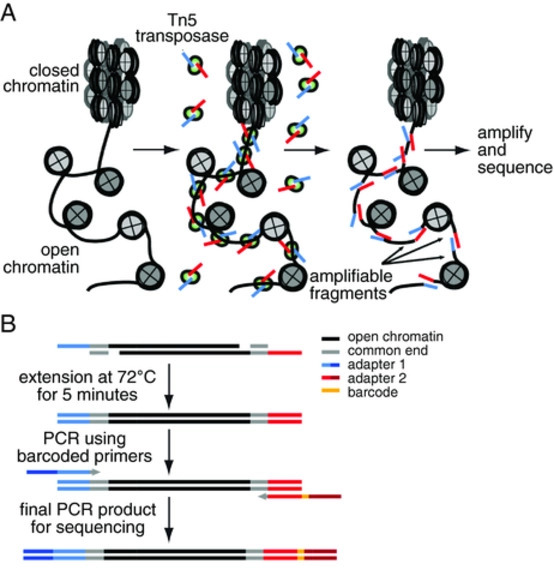
\includegraphics[width=0.5\textwidth]{plot/ch1/atac.jpg}
    \slcaption{ATAC-seq protocol schematic adopted from \cite{Buenrostro2015a}}
    \label{fig:atac}
\end{figure}

The ATAC-seq assay is conceptually a simple adaptation of the typical NGS procedure, and as previously mentioned relies on strategic sheering of the genome (in this case, targetted amplification) followed by sequencing. Here, a hyperactive Tn5 transposase enzyme preferentially accesses the sequence not wrapped in nucleosomes, inserting sequencing adaptors that can be directly amplified. This results in fragments of DNA whose length follows a bimodal distribution, with the majority derived from the space between nucleosomes and tending to be short, and the minority spanning a nucleosome and thus having a fragment length of at least $\sim$150 base pairs \cite{Yan2020a}. Since the amplified pieces of sequence predominantly appear in regions without nucleosomes, identifying "accessible" regions (for a given threshold) is an exercise in statistical detection of regions with signal enriched over the background.

The concept behind ATAC-seq is similar to previous assays for chromatin accessibility such as MNase-seq and DNAse-seq which use micrococcal nucleases, and DNAse 1 enzymes to fragment the sequence respectively \cite{Bell2011a}. FAIRE-seq, a successor to DNAse-seq introduced in \textcite{Giresi2007}, performs a fundamentally different fragmentation by isolating DNA that is not able to be experimentally cross-linked to nucleosomes. In contrast to MNAse-seq and DNAse-seq, ATAC-seq requires far fewer experimental steps and isolated cells, allowing for efficient study of small populations of cells (as shown by \textcite{Buenrostro2015a}) while comparisons with FAIRE-seq show substantial bias in the latter towards enhancer and intronic elements and a smaller enrichment of signal over the sequencing background \cite{Tsompana2014}. This makes ATAC-seq an experimentally efficient procedure for generating high coverage chromatin accessibility tracks in low to moderate numbers of cells. DNAse-seq was adopted enthusiastically by consortia such as \textcite{ENCODEProjectConsortium2012} and substantial effectively-legacy data exists from this assay, however more recent efforts in the same groups (i.e. \textcite{Moore2020}) are focusing on ATAC-seq for this task. The analysis of ATAC-seq data therefore remains a valuable task, especially as the number of generated datasets continues to increase year over year (\textcite{Yan2020a} demonstrates this up until 2019).

\subsubsection{Chromatin immunoprecipitation followed by sequencing} \label{intro:chip}

Both the combinatorial binding of transcription factors and post-translational modification of histone proteins are key players in the complex logic of gene expression \cite{Farnham2009}. Transcription is regulated by a large number of \glspl{cre} categorized by function and distance to the \gls{tss}. These include promoters and promoter-proximal elements, enhancers, silencers, insulators, and boundary elements for topologically associated DNA domains (reviewed in \textcite{Wittkopp2011}). Many transcription factors bind to specific patterns in DNA called ``motifs'', however the majority have either a non-specific binding sequence or none at all, leading to the desire for an experimental approach to determine where specific transcription factors are bound in specific cellular contexts \cite{Spitz2012}. At the same time, specific covalent modifications to histone proteins have been shown to be enriched at active enhancer and promoter elements, indicating their involvement in the recruitment of proteins for transcriptional activation. For the purposes of this thesis, only a handful of the many histone modifications are necessary for the putative identification of enhancer and promoter regions (\Cref{fig:histones}). In the following and throughout, the nomenclature for histone modifications is the histone that is modified (Histone H3 = H3), the residue that is modified (lysine residue 4 = K4), and the actual modification (me1 = mono-methylation, me3 = tri-methylation, ac = acetylation) such that, for example, mono-methylation of the fourth lysine residue on histone protein H3 would be denoted as H3K4me1 \cite{Gates2017}. A summary of important histone modification follows.

\begin{figure}
    \centering
    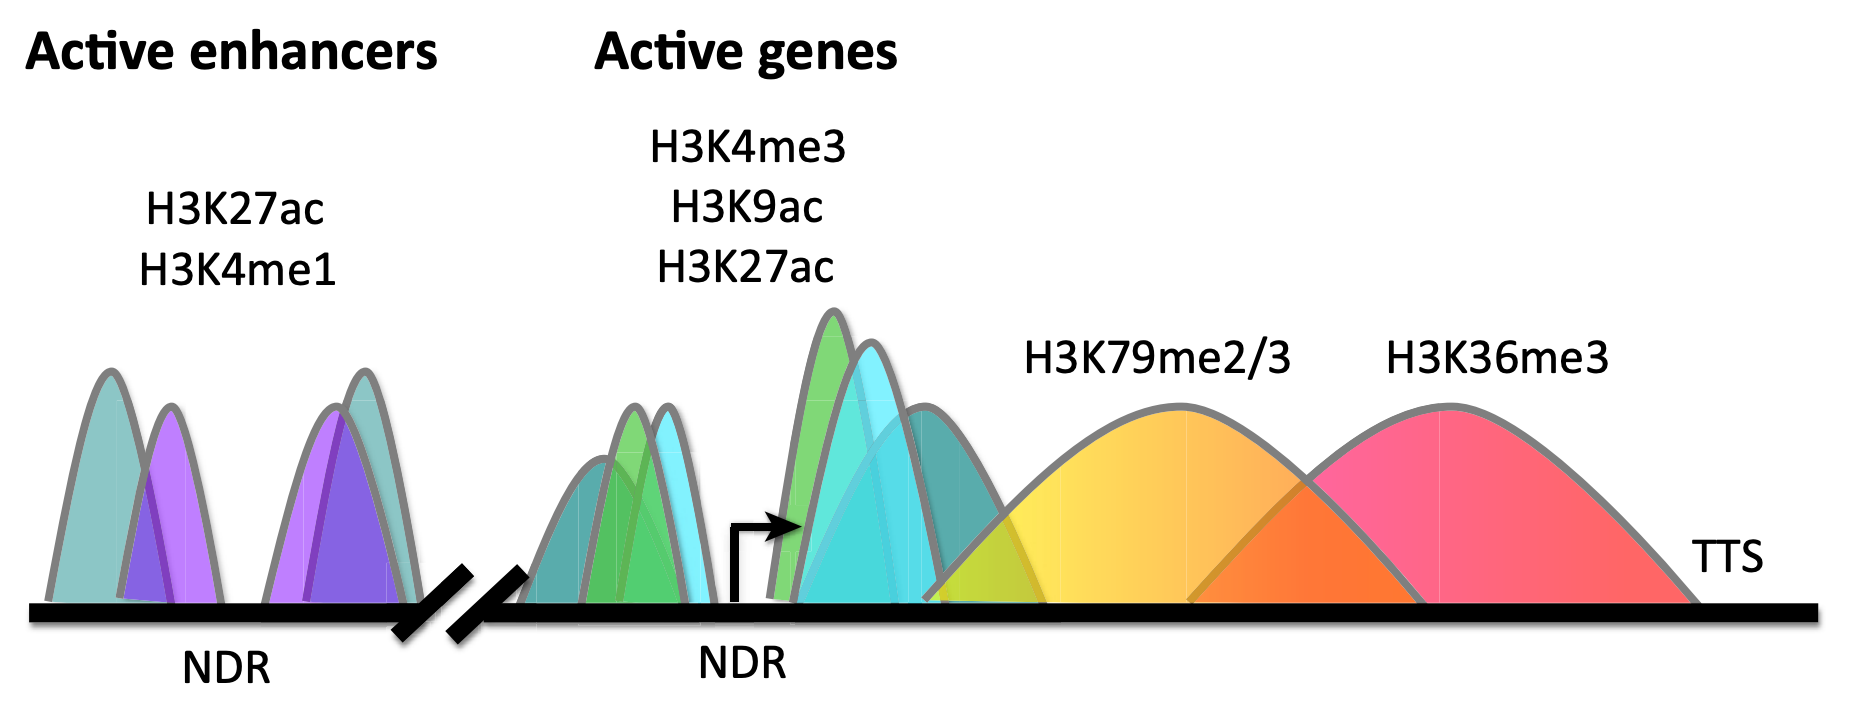
\includegraphics[width=\textwidth]{plot/ch1/histones}
    \slcaption{Typical eukaryotic ChIP-seq defined active enhancer, promoter, and gene body histone modifications from \textcite{Gates2017}. H3K4me3 and H3K9ac typically load onto active promoter regions, while H3K79me2/3 and H3K36me3 are found on the actual gene body being transcribed. H3K27ac loads onto both active promoters and enhancers, while H3K4me1 is found predominantly on the latter. These are all generalizations, and represent typically found patterns. NDR = nucleosome-depleted (accessible) regions, NDR = nucleosome depleated region (i.e. accessible chromatin).}
    \label{fig:histones}
\end{figure}

\paragraph{H3K4me1} is found predominantly at enhancer elements \cite{Gates2017}. Recent evidence suggests that H3K4me1 can also be found in promoter elements, with a bimodal pattern flanking H3K4me3 in active promoters and unimodal peak, coinciding with H3K4me3 and H3K27me3, proximal to the \gls{tss} in poised promoters \cite{Bae2020}.  

\paragraph{H3K4me3} is typically believed to be the distinguishing mark of promoter elements \cite{Gates2017}. Typically, the dynamic regulation of methylation between DNA methylation, H3K4me1, and H3K4me3 is able to alter to state of a region from functionally inactive to enhancer or promoter elements respectively \cite{Sharifi-Zarchi2017}. Interestingly though, H3K4me3 occasionally is observed on putative ``super enhancers'', especially in some cancers, though this relationship is the subject of much debate \cite{Li2019}.  

\paragraph{H3K27ac} is an activity marker found at both active enhancers and promoters \cite{Gates2017}.

\paragraph{H3K79me2/3} as in, either the di or tri methylation of H3K79, is uniquely deposited by the \gls{dot1l} protein, and is often found within the body of actively transcribed genes and is associated with transcriptional elongation \cite{DJ2008,Q2002a}. While not usually found at enhancer elements, recent evidence strongly suggests a role for DOT1L mediated H3K79 methylation in enhancer-promoter interactions in cancers caused by \gls{mll} fusion proteins, which is of interest to results later in this thesis \cite{Godfrey2019a}. 

\paragraph{H3K27me3} functions as a repressive mark for gene expression and is found at silencer elements \cite{Cai2021, Gates2017}. 

These marks vary across the genome depending on a large number of biological factors; ChIP-seq provides an empirical tool to measure their presence. 

ChIP-seq combines chromatin immunoprecipitation (ChIP) with NGS sequencing to identify protein-DNA interactions on a genome-wide scale \cite{Park2009a}. ChIP involves the covalent crosslinking of DNA to any associated proteins followed by the random fragmentation of the genome; specific antibodies are used to ``pull down'' regions bound by a specific protein or histone modification, and the remainder are washed away \cite{Nakato2021,Furey2012}. The remaining fragments of DNA are annealed to sequencing primers and amplified. The effect of this procedure is to enrich sequenced regions for areas of the genome bound by a specific protein. Typically, ChIP-seq experiments are paired with an ``input'' run, in which the pull down step is not performed, in order to assess the genomic background of enriched regions. These are typically removed from the analysis and peak calling as they represent technical artefacts and not biologically relevant DNA-protein complexes. 

\subsection{Specific Machine Learning Applications for Functional Genomics}

\subsubsection{Identifying Signal Enrichement (Peak Calling) with Machine Learning} \label{intro:pc}

One of the key tasks after performing ATAC-seq or ChIP-seq is to determine regions which are enriched for signal over the background \cite{Yan2020a}. Many approaches have been developed for this task (partially reviewed and benchmarked in \textcite{R2017}) based on statistical models typically modelling signal to noise ratios according to a Poisson distribution. This model appears to correctly discriminate visually enriched peak regions, though both the false positives and false negative identifications are frequently thought to be bottlenecks in analyses that rely on discretized region sets. Recently, a deep learning based peak called was proposed which appears to exceed the performance of the gold standard approach, MaCS2 \cite{Hentges2021a,Zhang2008,Gaspar2018}. The model relies on a wide-and-deep convolutional neural network trained on a manually curated set of 8463 peaks from various \textcite{ENCODEProjectConsortium2012} datasets and 8503 noise regions \cite{Cheng2016,Hentges2021a}. 

\subsubsection{Chromatin State Annotation}

After sequencing and discretizing histone modifications into peak regions, a researcher may wish to annotate the genome of their cell type of interest with putative states (i.e. active or poised enhancer or promoter, heterochromatin, etc.). Due to the high dimensionality of the data (a number of chromatin marks each with a genome-scale coverage track), this is a difficult task to perform manually. \textcite{Ernst2012} discovered that by modelling the chromatin state along the genome as a Markovian process, inference of putative states can be efficiently performed with standard approaches such as \glspl{hmm}. ChromHMM and extensions have remained standard approaches for chromatin state annotation and the identification of putative enhancer regions across cell types of interest \cite{Ernst2017}. However, latent states require manual annotation which is often non-trivial, and in the case of niche cell types it is often difficult to generate the required ChIP-seq data for manual annotation. The alternative approach, using an imputation program such as ChromImpute leads to variable quality of input data heavily depending on the sequence specificity of the given mark \cite{Ernst2017}.  Topic modelling represents an attractive alterative that relies solely on accessible chromatin to annotate shared and distinct regulatory elements, and has been successfully used for single cell ATAC-seq data \cite{BravoGonzalez-Blas2019}. ATAC-seq is comparably cheaper and easier to assay in niche cell populations, and a wide array of public reference data is available from consortia.  However, a satisfying adaptation of the cisTopic \gls{lda} approach has never been attempted for bulk ATAC-seq in specific populations of cell types. In order to determine shared and distinct regulatory elements in closely related cell types, topic modelling represents a viable approach which has previously been demonstrated effective in a single cell context.

\section{Thesis Aims}

The overarching goal of this thesis is to develop machine learning methods to interpret next generation sequencing data and apply them to two specific questions. The two sections above give background information on the motivation for solving the problem of inferring directional migration from whole genome sequencing data (\Cref{intro:popgen}) and identifying shared and distinct regulatory elements in closely related celltypes (\Cref{intro:fungen}). For this second question, we develop a topic modelling approach based on \gls{lda} for bulk ATAC-seq data. We apply this approach to a specific form of leukemia with a poorly understood regulatory landscape and uncover a specific set of enhancer elements with novel histone modification profiles. This thesis both represent methodological advances in two different sub-fields and the contribution of novel results, namely the identification of an ancient back-migration and a subset of PAF1c bound enhancer elements in MLL-AF4 leukemia. A summary of the chapters follows.

%Chapter 2 introduces \gls{smc2} and applies it to the problem of detecting ancient migration into Africa.  Chapter 3 develops the \gls{blda} algorithm and demonstrates its use on simulated and real data. Chapter 4 applies BLDA to an unknown dataset of MLL-AF4 patients and cell lines in an attempt to study active regulatory programs in these samples. Chapter 5 discusses the overall implications of and next steps with this research.

\paragraph{Chapter 2} describes the \gls{smc2} method for sampling from the posterior distribution of \glspl{arg} conditioned on genomic variation from \gls{wgs} data and inferring demographic parameters including population-specific effective population size and directional migration rates over time. I use simulation to demonstrate the accuracy and limitations of inference and apply the method to analyse individuals from the \gls{sgdp} and \gls{hgdp}. In doing so, I discover a substantial back-migration from the ancestors of non-Africans to the ancestors of present day Africans between 40 and 70 thousand years before present. The remainder of the chapter investigates the dynamics and magnitude of this migration, and explores its ramifications on human origins.  

\paragraph{Chapter 3} introduces the \gls{blda} method for performing topic modelling on bulk ATAC-seq data. This method is a direct extension of the cisTopic LDA approach taking into account a quantitative rather than binary signal for read density at peak regions. I show that BLDA is as effective in statistically pseudobulked ATAC-seq samples as cisTopic is in single cell ATAC-seq data. Additionally, I show that LanceOTron's deep learning peak caller results in cleaner inference in a range of topic modelling applications. I use the developed approach on a curated set of sorted cell types representing the differentiation pathway of haematopoiesis and erythopoesis and show that BLDA is superior to a naive implementation of cisTopic, and additionally recovers known regulatory prorgams active in these cell types.

\paragraph{Chapter 4} applies the previously developed \gls{blda} method to a set of MLL-AF4 driven leukemia patients and cell lines and demonstrates a unique and shared set of differentially accessible chromatin regions when compared to a specifically selected set of closely related B cell progenitors. These differentially accessible regions are hypothesized to represent unique regulatory programs that distinguish the cells. I isolate key regions of these regulatory topics and show that they are highly robust against the stochastic inference procedure. I model these cell types alongside blood cells from the ENCODE consortium and demonstrate their distinctiveneess. I compare these regions against ChIP-seq for known histone modifications and show that they are marked as putative enhancers without the DOT1L signature typical of enhancers in MLL-AF4 leukemia, and additionally bound by PAF1c. I show that these regions share activity profiles with certain haematopoietic progenitor cells and elaborate on future experimental validation to elucidate their exact function in MLL-AF4 leukemia.  

\paragraph{Chapter 5} discusses the contribution of these results to their respective areas and suggests further work.

%Machine learning is an umbrella term encompassing a wide variety of algorithms that are designed to learn complex patterns in data to solve a task. These methods often involve, at least partially, statistical inference of parameter values for an underlying generative process that can be used to either better understand the process itself or predict the process in the future for different data \cite{Bzdok2018}. This often, but not always, involves learning parameter values from training data and validating the inferred model on unseen validation samples. Machine learning has seen wide adaptation in genomics due to the breadth and complexity of available datasets. Some examples include:



%The method used to infer demographic history from WGS in PSMC is a hidden Markov model, a machine learning model which attempts in this case to learn the distribution of \gls{tmrca} between two alleles along the genome using information about the mutations present in each sample. 




%This model was the first to utilize \gls{wgs} to infer important aspects of human history, notably observing a large bottleneck in Eastern and Western Eurasian populations before 20 \gls{kya} and early population diversification in Africa between 100-120 kya \cite{Li2011a}. These estimates would be refined in later years as methods and data quality simultaneously improved, but the inferences from PSMC played a key role in beginning the genomics era of genetic anthropology.   

% Modern methods 
%As


% \textcite{Griffiths1997a} showed that to incorporate recombination into the coalescent required only a small extension to the gene geneology. This is especially important given the large amount of biologically relevant auto-correlation in the genome, also known as linkage disequilibrium. 

% Previous work on polymorphism data including its limitations. Some results.
% Modern methods in population genetics like ArgWeaver, MSMC, etc. 
% Statement about the lack of any methods which can infer time varying migration and the desire for these methods to simultanesouly infer a coloured ancestral recombination graph. 

% or collectively the \gls{arg \cite{Griffiths1997,Wiuf1999}}



% Here a sequence will refer to the ordered set of bases representing a single strand of the molecule.

%New ,machine learning methods capable of learning many different demographic parameters from small numbers of individuals. 

%The interplay between genetics and ant

%have allowed for the development of efficient inference algorithms which combined with these new data sources are allowing us to understand the origins, dispersal, and interactions of global populations \cite{Hodgson2010}. 



% These efforts are already uncovering millions of private variants from non-European populations, paving the way to understand genetic risk factors for disease in ethnically diverse populations \cite{McGuire2020,Choudhury2017}. 

% As a downside, mention that the error rates per base are much higher than with sanger sequencing \cite{Liu2012}
% Talk about long read versus short read, and arrays versus sequencing.

% dideoxynucleotides (remove 3' hydroxy group atom) stop extension, chain terminating nucleotide is identified with a fluorescent dye at the 3' end. Extension products are seperated by capiliary electrophoresis or on a slab gel traditioanlly , where an electrical field moves the DNA with a speed inversely proportional to its molecular weight. Excited terminal bases emits light which can be recorded. Remains gold standard with extremely high accuracy. Sequencing single genes, microsatellite or STR, hard to sequence regions. 

% NGS transformed this. Massively parrellel versus one forward and reverse read.  Interogating > 100 genes, low input amounts, novel variants, 

% - library obtained either by amplification or by ligation 

% - Four main methods used by NGS systems
%     - Pyrosequencing
%         - Each nucleotide incorporation releases a pyrophosphate, used in a series of reactions resulting in light which is recorded by a camera. 
%         - Comparable read lengths to sanger, but high error rates over homopolymers.
%     - sequencing by synthesis (most popular, Illumina HiSeq)
%         - illumina
%         - All 4 nucelotides are added and terminated, one binds, the base is read by fluorsence, then the attached termination and fluorsence is washed away and the process is repeated. 
%         - increased read lengths as you get longer due to incomplete deletion of the fluorsence
%     - squencing by ligation
%         - 16 oligo nucleotide probabilities
%         - adaptor is bound, and the 2 specific bases of the oligose are bound with the fluorecent probe. The probe and last 3 bases are washed away and the sequence is repeated for 5 adaptor sequences offset by one base
%         - very short reads
%     - ion semiconductor sequencing 
%         - semiconductor transistor can detect phases
%         - a single H+ is released on base incoroporation. base calling is a NN, like gerton's previous work 
%%\begin{savequote}[8cm]
%\textlatin{Neque porro quisquam est qui dolorem ipsum quia dolor sit amet, consectetur, adipisci velit...}

%There is no one who loves pain itself, who seeks after it and wants to have it, simply because it is pain...
%  \qauthor{--- Cicero's \textit{de Finibus Bonorum et Malorum}}
%\end{savequote}

\chapter{\label{ch:1-smc2} A particle filter for demographic inference} 

\minitoc


%%\begin{savequote}[8cm]
%\textlatin{Neque porro quisquam est qui dolorem ipsum quia dolor sit amet, consectetur, adipisci velit...}

%There is no one who loves pain itself, who seeks after it and wants to have it, simply because it is pain...
%  \qauthor{--- Cicero's \textit{de Finibus Bonorum et Malorum}}
%\end{savequote}

\chapter{\label{ch:1-aaa} Ancient Admixture into Africa from the Ancestors of non-Africans} 

\minitoc




\begin{quote}
    \noindent \small Genetic diversity across human populations has been shaped by demographic history, making it possible to infer past demographic events from extant genomes. However, demographic inference in the ancient past is difficult, particularly around the out-of-Africa event in the Late Middle Paleolithic, a period of profound importance to our species' history.  Here we present {\tt SMCSMC}, a Bayesian method for inference of time-varying population sizes and directional migration rates under the coalescent-with-recombination model, to study ancient demographic events. We find evidence for substantial migration from the ancestors of present-day Eurasians into African groups between 40 and 70 thousand years ago, predating the divergence of Eastern and Western Eurasian lineages.  This event accounts for previously unexplained genetic diversity in African populations, and supports the existence of novel population substructure in the Late Middle Paleolithic. Our results indicate that our species' demographic history around the out-of-Africa event is more complex than previously appreciated.
\end{quote}

\newpage

\printglossary

\section{Introduction}

Methods to characterize demographic history from genetic data alone form a useful and independent complement to archaeological approaches \cite{Nielsen2017a}, and many methods have been developed for this purpose \cite{Li2011,Pickrell2012,Rasmussen2014,Schiffels2014,Mathieson2014,Steinrucken2015,Malaspinas2016,Chikhi2018,Speidel2019,Kelleher2019,Wang2019a,Albers2019}. 
A particularly interesting time in human history is the end of the Middle Paleolithic approximately $\sim$60 \gls{kya}, which saw the divergence of the most deeply sampled lineages of human genetic variation, introgression from multiple archaic sources, and the expansion of anatomically modern humans \gls{ooa}. 
As archaeological evidence and ancient DNA from this period are scarce, inference of demography from present-day genetic data is potentially very informative, though technically challenging. Here, we use the previously developed approach, \gls{smc2}, to infer population size and directional migration in a unique and dynamic period of ancient human development.

This section is structured as follows. Firstly, I give an introduction to pertinent historical and anthropological theories relating to this period of time so as to orient the reader. Secondly, I introduce competing approaches for the inference of ancestral recombination graphs and motivate the usage of \gls{smc2} for this application. Following this, I outline my contributions to this area of research, which involve the identification and characterization of a putative directional migration from the ancestors of modern day Eurasians to the ancestors of modern day Africans. 


\subsection{Out of Africa and the peopling of Eurasia}

An abundance of archaeological and genetic evidence has shown that the continent of Africa is the historical source of all modern humans \cite{Lopez2015}. The continent contains within it more genetic sequence diversity than any other region of the world, so much so that the two haplotypes of a single African genome are less similar than any two haplotypes outside of the continent \cite{Mallick2016}. The population structure in the continent has its roots in the transition from the middle to late Pleistocene, with hunter gatherers groups from Southern Africa including the Khomani San and Ju'|Hoan diverging in large part from the remainder of modern African populations between 200 and 250 \gls{kya} \cite{Lipson2019}. Additionally, recent evidence suggests that deeply diverged archaic lineages have substantively contributed to at least some modern Western African populations \cite{Durvasula2019}. Populations on the content were, therefore, highly structured and geographically localised many tens of thousands of years before we have evidence for the first \gls{amh} leaving the continent.    

Evidence from climate science suggests that a combination of a gradual shift away from aridity in Northern Africa as well as short term dry-wet cycles may have motivated both global and local range expansions \cite{Schaebitz2021, Timmermann2016}. The most pertinent of these range expansions is the migration \gls{ooa} and into Eurasia, an event which will form the basis of modern population structure around the globe. These migrants were probably diverged from sister populations within the continent for many tens of thousands of years before their eventual dispersal into the Levant and beyond \cite{Bergstrom2019, Schiffels2014}. Though these individuals were by far the most successful group of migrants, some fossil evidence exists placing \gls{amh} in regions of the globe such as Fuyan cave in China between 80 and 120 \gls{kya}, between 63 and 73 \gls{kya} in Sumatra, and 65\gls{kya} in Australia, all of which would be earlier than explainable with this single migration; however, genetic analysis of diverse populations has yet to identify any solid evidence for these earlier migrations contributing to modern diversity \cite{Skoglund2018}.

The population which formed this successful range expansion out of Africa experienced at least one, and potentially multiple, breeding events with Neanderthals \cite{Sankararaman2012}. Eventually, the group split into two distinct subpopulations around the time of the Ust'-Ishim individual, approximately 45 \gls{kya} \cite{Fu2014}. One of these populations went East, forming the basis of for East Asians and Aboriginal Australians, while the other went West, forming the initial Upper Paleolithic European hunter gatherers \cite{Skoglund2017,Lipson2017}. These were not the only derivative groups from the original \gls{ooa}, as another earlier diverged population popularly known as ``Basal Eurasians'' are thought to have branched before the initial contact with Neanderthal populations and contribute to later European population structure \cite{Lazaridis2014}. From this point on, diversification occurred on a highly regional basis, beyond the scope of this brief review. 

Many questions about this process of diversification remain unanswered, however. 

% Remaining questions about how these groups interacted...? What about other theories of the back migration?

\subsection{The Ancestral Recombination Graph (ARG) and admixture inference in the ancient past}

The phylogenetic trees over a set of samples as they change along the genome through recombination, collectively referred to as the ancestral recombination graph (ARG) \cite{Griffiths1997a,Rasmussen2014}, record all information about the samples' evolutionary history.  This history itself is shaped by the population's demography, a statistical relationship that is quantified by the coalescent-with-recombination (CwR) model \cite{Griffiths1997a}.  The ARG is a complex data structure which is only weakly constrained by the observed genetic polymorphisms, making inference of demography difficult. By making approximations to the CwR, for instance by making an independent-sites assumption, efficient parametric inference of demography becomes possible \cite{Excoffier2013,McVean2005}.  Methods including {\tt PSMC} \cite{Li2011}, {\tt diCal} \cite{Steinrucken2015} and {\tt SMC++} \cite{Terhorst2015} allow non-parametric inference of demography under a closer approximation to the CwR, but one that does not include gene flow between populations. {\tt MSMC} \cite{Schiffels2014} introduced the cross-coalescent rate and {\tt MSMC-IM} described how to interpret this rate in the context of a isolation-migration model to estimate a migration rate between populations\cite{Wang2019a}. However, these methods are not well suited for estimating directional migration rates. 

Here we extend {\tt SMCSMC} (Sequential Monte Carlo inference of the Sequentially Markovian Coalescent, \cite{Henderson2018}) to allow inference of directional migration.  {\tt SMCSMC} is a Bayesian method that uses a particle filter to explicitly sample from the posterior distribution of ARGs over multiple diploid samples under the full CwR model.
Since particle filters operate by simulating latent variables (here the ARG) under the statistical model of interest, it becomes possible to handle complex demographic scenarios.  We exploit this by extending the CwR model to include time-varying directional migration rates in a two-island demographic model.  We use the posterior sample of ARGs including migration events to update the parameters of the demographic model, using either expectation-maximization or a variational Bayes procedure, and iterate these steps until convergence.   We apply {\tt SMCSMC} to estimate directional migration rates in whole genome sequencing data from the Simons Genome Diversity Panel (SGDP) \cite{Mallick2016} and the Human Genome Diversity Panel (HGDP) \cite{Bergstrom2019} to investigate population structure around the OoA event.

\section{Results}

\paragraph{Substantial Migration from Eurasian to African Ancestors} We use {\tt SMCSMC} to analyse pairs of individuals from the SGDP and simultaneously infer migration rates and effective population sizes ($N_e$) under a two-island model with directional migration.  Population sizes and migration rates are modeled as piece-wise constant across 32 exponentially spaced epochs from 133 to 133016 generations in the past, corresponding to 3.8 thousand to 3.8 million years ago (3.8kya--3.8Mya) using a generation time $g=29$ years \cite{Fenner2005}.  We find that the method infers high rates of migration from descendants of the OoA event ('non-Africans') to Africans, but not in the opposite direction, in the period $30$--$70$kya corresponding to the Late Middle Paleolithic (Fig.\ \ref{migrationplot}). In populations from the Niger-Kordofanian and Nilo-Saharan language groups, comprising the majority of the population on the African continent, the peak inferred migration rate from Eurasian populations ($2.5$--$3.0\times 10^{-4}$ and $3.5$--$4.0\times 10^{-4}$, in units of proportion of the target (ancestral African) population replaced per generation) most frequently falls in the epochs spanning 35--45kya, while peak migration rates in the opposite direction are substantially lower ($0.5$-$1.0\times 10^{-4}$) and occur earlier, in the epochs spanning $55$--$70$kya (Supplemental Fig.\ \ref{fig:peaks}). Populations in the Afroasiatic language group show evidence of large amounts of directional migration in the Holocene (Supplemental Fig.\ \ref{sgdp_mig}), which is consistent with previous findings of relatively recent European introgression into these populations \cite{Busby2016, Fan2019}. 

To assess the impact of errors introduced by statistical phasing, which was used to phase the SGDP data, we repeated the analyses above on a subset of physically phased individuals from the Human Genome Diversity Project (HGDP) \cite{Mallick2016} (Supplemental Section \ref{hgdp_section}). This data set comprises individuals from four African (Yoruban, San, Mbuti, and Biaka) and nine non-African populations (Druze, Han, Karitiana, two Papuan populations, Pathan, Pima, Sardinian, and Yakut). {\tt SMCSMC} results in the HGDP are qualitatively similar to those in the SGDP (Fig.\ \ref{migrationplot}b, Supplemental Fig.\ \ref{fig:peaks}a). Inferred migration rates are, in general, lower in HGDP data than when using matched SGDP samples (Figs.\ \ref{migrationplot}a,b and \ref{fig:both}, demographic inference in matched sampled in Supplemental Fig./ \ref{fig:hgdp_sgdp}), but in all cases, the migration rates from Eurasia to Africa are substantially higher than in the opposite direction, consistent with the findings in the SGDP (Supplemental Fig.\ \ref{fig:both}). 

We asked whether {\tt SMCSMC} has power to detect a large back-migration event in the Late Middle Paleolithic and distinguish it from other demographic scenarios. To answer this we used {\tt SCRM} \cite{Staab2015} to simulate a gigabase of sequence data under a two-island demographic model,
%with a split time of 385kya,
with effective population sizes chosen to be comparable to typical African and Eurasian populations as inferred from real data. 
%We simulated an early split time to allow {\tt SMCSMC} to resolve the split times of the populations without undue bias. \textcolor{red}{\bf This explanation sounds weak.  It suggests that we're making simulating an easier case than reality, throwing doubt on our simulations.  Thoughts?} 
To this we added a $10$ky pulse of forward, backward or bidirectional migration of varying strengths, with the midpoint of the migration pulse within the range $40$ to $70$kya.  To quantify the inferred amount of migration we calculate the integrated migration fraction (IMF), defined as one minus the probability that a lineage in the destination (e.g.\ African) population traced backwards in time remains in that population across a given epoch according to the migration model (see Methods).  For the simulations, we chose the most recent 100kya as epoch, and used scenarios with IMFs ranging from $0$ to $0.593$. For each simulation we report the inferred IMF in both the forward and backward direction (Fig.\ \ref{fig:sim}); full results are given in Supplemental Section \ref{simproc}.  We find that {\tt SMCSMC} has good power to detect backward migration pulses up to $60$kya (median ratio of inferred and true IMF, $0.91$), while power drops off at $70$kya (IMF ratio $0.46$). In the pure backward migration case, some forward migration is falsely inferred, but this is always substantially less than the inferred backward migration (median ratio inferred forward to true backward IMF, $0.37$; true migration peak $\leq 60$kya).  However, in the case of true forward migration as well as bidirectional migration, roughly equal mixtures of forward and backward migration are inferred (Fig.\ \ref{fig:sim}). We conclude that in the epoch $40$--$70$kya the forward and bidirectional scenarios are difficult to distinguish from each other, but both can be distinguished from backward migration, the only scenario resulting in substantially different inferred backward and forward migration.

To validate the existence of the migration pulse, though not its direction, we next analyzed the same data using MSMC, which is widely used to estimate gene flow in the ancient past by estimating the relative cross-coalescent rate (RCCR) between two populations \cite{Schiffels2014,Fan2019, Pagani2015, Raghavan2015}. We use the updated implementation MSMC2 recommended by the authors and first published in \cite{Malaspinas2016}. Each of the {\tt SMCSMC} analyses are repeated using MSMC2 to estimate effective population size and RCCR (Supplemental Figs.\ \ref{sgdp_mig}, \ref{fig:both}, \ref{sgdp_ne}). Consistent with previous analyses conducted with MSMC2, our estimates show high RCCR in the Late Middle Pleistocene in both the SGDP and the HGDP (Fig.\ \ref{migrationplot}c,d) \cite{Fan2019, Bergstrom2019}. These observations confirm the existence of a substantial pulse of ancient gene flow between Eurasians (Han Chinese) and Africans.

\paragraph{Migration Pre-dates East-West Eurasian Divergence}

To assess whether the inferred back-migration shows variation across the descendants of the OoA event, we repeated the analyses using three representative non-African groups in the SGDP: Han Chinese, French European, and Papuans.  Since simulations show that {\tt SMCSMC} has little power to detect migration predating 70kya, and to exclude Holocene migration, the epoch we use to calculate real-data IMFs comprise the period of peak inferred migration up to the period of diminishing power (30--70kya); we use this epoch for all subsequent analyses. Inferred IMFs are not significantly different between Han Chinese and European populations in non-Afroasiatic populations (p=0.14, two-tailed paired t-test; Figs.\ \ref{migrationplot}h and \ref{sgdp_heatmap}, Table \ref{average_sgdp_migration_table}), consistent with migration occurring before the European-East Asian split approximately 40kya \cite{Mathieson2014}.  The contribution of this admixture event to extant African genetic variation is substantial; the estimated IMFs indicate that for individuals in the major African language groups, approximately a third of ancestral lineages trace their ancestry through the proto-Eurasian population (Niger-Kordofian group, $0.35\pm 0.04$; Nilo-Saharan groups, $0.41\pm 0.03$; Table \ref{average_sgdp_migration_table}). When we estimate these proportions using a Papuan sample to represent non-African descendants we find slightly but significantly smaller values compared to estimates using either the Han Chinese or European populations (mean difference of $0.029 \pm 0.002$, p=9.2$\times$10$^{-15}$, and $0.025 \pm 0.004$, p=$2.3\times 10^{-10}$, paired t-tests, Supplemental Table \ref{average_sgdp_migration_table}, \ref{sgdp:papuan_imf}). Similarly, in the HGDP, inferred migration in both Papuan groups (Sepik and Highlands) was 0.025 $\pm$ 0.004 (p=$1.4\times10^{-6}$) lower than French and Han (Supplemental Table \ref{hgdp:papuan_imf}).  We comment on this observation in the Discussion. 

\paragraph{Directional Migration Explains Excess Inferred African Genetic Diversity 100kya} Previous studies looking at effective population sizes ($N_e$) in human ancestral populations have consistently reported inflated inferences in African populations approximately 100kya, often hypothesized to be due to unaccounted-for population substructure within Africa \cite{Li2011,Schiffels2014}. We use {\tt SMCSMC} to analyze African individuals paired with an individual from one of three non-African populations (Han Chinese, French European, and Papuans) and infer $N_e$ for the African ancestral population under a two-island model with directional migration.  Each analysis was repeated three times to assess the contribution of stochastic sampling to the inferences (Figs.\ \ref{neplot}, \ref{sgdp_ne}, per population $N_e$ in Supplemental Fig. \ref{fig:individual_pop_sizes}). {\tt SMCSMC} infers substantially lower African $N_e$ than {\tt MSMC} in the period $80$kya--$300$kya.  In addition, while {\tt MSMC} inferences show convergence of African and Eurasian ancestral $N_e$ estimates only around $300$kya, inferences from {\tt SMCSMC} indicate convergence at $150$kya (Fig.\ \ref{neplot}a), closer to the hypothesized time of the diversification of the ancestral lineages prior to the main out-of-Africa migration episode \cite{Timmermann2016, Malaspinas2016}. The same analysis on physically phased samples from HGDP show that these results are not driven by errors due to statistical phasing (Fig.\ \ref{fig:both} and Supplemental Section \ref{hgdp_section}). When we used {\tt SMCSMC} to infer both African and European $N_e$ under a single-population model without migration, $N_e$ estimates were comparable to those from {\tt MSMC} (Fig.\ \ref{neplot}b), indicating that the {\tt SMCSMC} inferences are not driven by methodological biases particular to {\tt SMCSMC}.

To more directly support the interpretation that the lower African $N_e$ inferred by {\tt SMCSMC} is due to appropriate modeling of directional migration, we again used coalescent simulation with {\tt SCRM} to investigate various migration scenarios and their effects on inferred African $N_e$. Using the simulation framework as above, we examine $N_e$ estimates inferred under a two-island model with migration, and in addition $N_e$ separately inferred for each of the two simulated populations under a single-population model (Supplemental Section \ref{simproc}).  Focusing on single-population inferences, we found that for simulated African populations that had received substantial migration from the simulated Eurasian population either through backward or bidirectional migration, inferred $N_e$ values indeed were substantially inflated compared to true values (Fig.\ \ref{neplot}c,d), while this effect was not seen when forward (African-to-Eurasian) migration was simulated (Fig.\ \ref{neplot}e).  
Similarly, single-population Eurasian $N_e$ estimates were inflated in the presence of forward and bidirectional migration, but not backward migration (Supplemental Figs.\ \ref{fig:backsim}--\ref{fig:fwdsim}).
In contrast, when using a model that includes migration, inferred African $N_e$ do not show inflation in any of the three scenarios (Fig.\ \ref{neplot}c-e). We conclude that the inferences from {\tt SMCSMC} and {\tt MSMC} are compatible with substantial back-migration from ancestral Eurasians into Africans, but not substantial bidirectional or forward migration.

\paragraph{Less Gene Flow to Central and South African Hunter-Gatherers} We infer substantial Eurasian back-migration into all African groups, however the inferred IMFs for individuals from Khoe-San populations are significantly lower than for any other group (difference with Niger-Kordofians, $0.14 \pm 0.02$, $p = 4.4 \times 10^{-14}$; difference with Nilo-Saharans, $0.20 \pm 0.03$, $p = 6.9 \times 10^{-9}$, two-tailed t-test, Table \ref{table:sgdp_pairwise}). To further support this observation we used {\tt MSMC} to estimate the relative cross-coalescent rate (RCCR) for several populations, and find evidence for gene flow between Yorubans and Eurasians that is not shared with the Khoe-San individuals in either the SGPD and the HGDP (Fig.\ \ref{migrationplot}c,d). These results are consistent across Eurasian donor populations (Fig.\ \ref{fig:hgdp_sgdp}). The Khoe-San individuals are particular outliers, whose ancestors are inferred to have experienced approximately half the amount of admixture seen in Nilo-Saharan and Niger-Kordofanian groups (Fig.\ \ref{sgdp_heatmap}). 
In addition, we find that the Mbuti and Biaka, both Central African hunter-gatherer populations, show levels of Eurasian gene flow that are intermediate between levels observed in the Khoe-San and Yorubans (Fig.\ \ref{migrationplot}a,b, Supplemental Table \ref{average_sgdp_migration_table}).  This is mirrored by inferred IMFs for Central African Hunter Gatherers, which are significantly lower than other Niger-Kordofanian groups (difference $-0.08 \pm 0.03$, $p = 1.2 \times 10^{-3}$, Table \ref{table:sgdp_pairwise}), possibly reflecting the proposed early split times of the Mbuti and Biaka from the remainder of ancestral African populations between 60 and 200kya \cite{Patin2017, Lipson2019}. 

\paragraph{No Evidence for Excess Neanderthal Ancestry} Previous studies have proposed that a backflow from Eurasia may have brought Neanderthal ancestry into African populations \cite{Chen2020}. To assess whether the proposed Late Middle Paleolithic back migration might have introduced Neanderthal material, we analyzed a Yoruban and a French individual using {\tt SMCSMC} to draw a sample from the posterior distribution of ARGs, isolated the marginal trees containing an inferred back-migration event in the epoch $30$--$70$kya, and reported the inferred admixture tracts (``segments'', Supplementary Section \ref{dstats_section}). To assess whether the identified segments are plausible, we confirmed that their length distribution is consistent with IMF and timing of the migration inferred by {\tt SMCSMC} (Supplemental Section \ref{dstats_section}.1, \ref{fig:length}), and, as expected, we found that these African segments with putative Eurasian ancestry tend to be more closely related to a Eurasian sample than another representative of the same African population (Table \ref{dstats:a1}, Supplemental Fig. \ref{fig:f3}, \ref{fig:f3_admix}) in a global dataset of modern and ancient individuals compiled by the Reich group (see URLs). Within these African segments that are likely enriched for material with Eurasian ancestry, we then used $D$ statistics \cite{Patterson2012} to identify enrichment for Neanderthal material compared to an African background. We find no evidence for gene flow with a Vindija Neanderthal on the Mbuti baseline, or when compared to a different Yoruban (Table \ref{dstats:a5}, \ref{dstats:a4}). We additionally find no evidence for increased affinity to the Vindija Neanderthal when compared to the Altai, as would be expected if the material were descended from admixing Eurasians (Table \ref{dstats:a6}). However, we find that restricted to the identified segments, $D$ statistics have power to detect evidence for the known admixture from Vindija into a French individual (Fig.\ \ref{dstats}), suggesting that lack of power does not explain the lack of evidence we find for Neanderthal admixture into Africans.  In addition, we find no differences in affinity to Neanderthals or Denisovans between the variants which fall in segments and the whole genome (Fig.\ \ref{dstats}d). Taken together, this suggests that Eurasian-derived segments of the African genomes are not enriched with Neanderthal material.

\section{Discussion}
We have developed an approach for estimating demographic parameters and ARGs from whole genome sequence data, which can handle inference in complex demographic models, and implemented this in the software program {\tt SMCSMC} \cite{Henderson2018}. We used {\tt SMCSMC} to investigate ancient migration rates and population substructure, and found evidence for a substantial admixture from ancestors of present-day Eurasian populations into African populations in the Late Middle Paleolithic.

Our analysis suggests that a population ancestral to present-day Eurasians contributed as much as a third of the genetic material in many modern African populations. We find no difference in inferred admixture proportions when using French Europeans or Han Chinese as extant representatives of the donor population, indicating that the admixing population must have split from the out-of-Africa population before the East/West Eurasian divergence, implying a lower bound on the timing of the admixture of approximately 40kya \cite{Mathieson2014}. It appears that our results suggest that the migrating population was more similar to present-day French and Chinese populations than to Papuans.  However, up to 5\% of the genomes of some present-day Papuans have been suggested to derive from archaic introgressions \cite{Sankararaman2016}, and these contributions will have reduced the inferred levels of admixture into Africans when using Papuans as a representative of the Eurasian ancestors.
The alternative explanation, of an earlier divergence of Papuans and Eurasian ancestors, is possible but contested; in light of documented Eurasian admixture into Oceania, the effects of this early isolation are likely to be small relative to the large confounding effects of Denisovan admixture \cite{Malaspinas2016, Nielsen2017a}.

The proposed period of admixture has biased previous inferences of the African population sizes. We show that including directional migration into the model resolves previously unexplained high inferred $N_e$ in the period $80$ to $300$kya. It is well known that effective population size estimates are biased in the presence of population substructure and migration \cite{Chikhi2018, Li2011}. We use simulations to show that the proposed admixture event indeed causes an increase in estimated $N_e$ in analyses that do not explicitly model migration.  Correctly modeling of directional migration recovers the correct $N_e$, and allows us to infer a more recent split time between the two populations than indicated by previous analyses, although we did not attempt to formally estimate this time of divergence.

We found that not all populations in Africa have been equally affected by the proposed migration event. While the ancestors of Niger-Kordofanian and Nilo-Saharan populations show evidence of similar levels of Eurasian admixture, the ancestors of Central African and South African hunter-gatherer populations show markedly lower levels.  The date of genetic diversification of both the Central Hunter Gatherers and Khoe-San (SAHG) is contested \cite{Lipson2019}, but a date of $100$kya has been proposed \cite{Schlebusch2012}, providing a putative upper bound on the main admixture event.  Our simulations indicate that {\tt SMCSMC} has little power to detect the impact of migration events occurring more than $70$kya, providing an additional upper bound on the time of the migration episode, or the fraction of it that left a sufficiently distinct imprint on extant genetic material.

Compared to the remainder of the Niger-Kordofanians and Nilo-Saharans on the one hand, and the SAHG populations on the other, the Mbuti and Biaka show intermediate levels of admixture. Of these populations, the Biaka show slightly higher levels of admixture than the Mbuti, which is likely due to the well-documented admixture from Western African groups not shared with the Mbuti \cite{Batini2011}. The lower levels of admixture in Mbuti and Biaka compared to Niger-Kordofian and Nilo-Saharan populations imply at least partial diversification of the former at the time of the migration, placing an upper bound on the timing. However, dating the diversification of these groups is difficult. Recent estimates using $f$ statistics place the split concurrent with the San in a large-scale early expansion 200-250kya \cite{Lipson2019}, while older data consistently report an earlier split time between 50 and 90 kya \cite{Patin2018}. Further clarity on the early structure and diversification of hunter-gatherer populations are necessary to interpret their interactions with Eurasian migrants. The  Afroasiatic populations on the other hand show high levels of admixture, which also appears to be of much more recent origin, and it appears likely that this is the result of extensive admixture from Eurasian populations during the Holocene \cite{Busby2016, Fan2019}. 

It has previously been suggested that Eurasian back-migration may be responsible for Neanderthal material in Africans \cite{Chen2020}; however, we find no evidence for enrichment of Neanderthal-like material in putatively Eurasian-derived genomic segments in Africans, indicating that Neaderthal introgression into Eurasians occurred after the African introgression event we study here, or that further population structure in the Eurasian ancestral population precluded substantial transmission of Neanderthal material into Africa.

Our findings are consistent with several other published observations. Migration rate estimates using {\tt MSMC-IM} revealed high levels of admixture at times comparable to our results \cite{Wang2019a}. The coalescent intensity function additionally shows similar histories between sub-Saharan African and Eurasian groups with high coalescent intensity in epochs consistent with our inference and those of {\tt MSMC-IM}, supporting both an early split between the groups and a substantial replacement of genetic material more recently than $\sim100$kya \cite{Albers2019}. Evidence has been mounting for multiple migrations into the Eurasian continent, possibly mediated by climatic drivers \cite{Timmermann2016, Pagani2016}. Eurasian backflow during the Holocene has been well established \cite{Lopez2015, GallegoLlorente2015}, but earlier migrations have also been proposed before based on observations of the spatial distribution of Y chromosome and mitochondrial haplogroups \cite{Altheide1997, Hammer1998, Cruciani2002, Chandrasekar2007, Cabrera2018, Hervella2016, Haber2019}. At the same time, evidence has been mounting for extreme heterogeneity in the history of sub-Saharan Africans, with several unsampled population theorised to have contributed at various points in the past \cite{Lipson2019, Durvasula2019, Speidel2019}. In light of these recent studies, the observations in this paper add to a growing body of evidence for complex population structure and migration surrounding the Out of Africa event leading to a substantial replacement of the African population in the Late Middle Paleolithic.  


\section{Methods}


\paragraph{A Particle Filter for Demographic Inference} Details of the Sequential Monte Carlo for the Sequentially Markovian Coalescent ({\tt SMCSMC}) algorithm have been previously published \cite{Henderson2018} (see the URLs for an implementation). Briefly, {\tt SMCSMC} builds an approximation of the posterior distribution of genealogical trees along the genome using a particle filter, a method also known as sequential Monte Carlo. It does so by simulating a number of sequences of genealogical trees (particles) under a fixed set of demographic parameters $\theta$, using the sequential coalescent sampler {\tt SCRM} \cite{Staab2015}. Simulated recombination events may change the local trees along the sequence. Particles are then weighted according to their conditional likelihood given observed polymorphisms.  To avoid sample depletion, the set of particles is regularly resampled, which tends to remove and duplicate particles with low and high weight respectively.  To further increase the efficiency of the procedure, the resampling procedure targets not the partial posterior distribution that includes polymorhpisms up to the current location, but also includes a "lookahead likelihood" term that approximates a particle's likelihood's dependence on subsequent polymorphisms, while ensuring that the estimate of the posterior tree distribution remains asymptotically exact.  From a sample of trees from the posterior distribution, Variational Bayes (VB) or Stochastic Expectation Maximization (SEM) is used to update the estimates of demographic parameters $\theta$. This is repeated over a given number of iterations, or until $\theta$ have converged.

To add the ability to infer time-varying migration rates, we exploit the capabilities of {\tt SCRM} to simulate ARGs under complex demographic scenarios, and collect sufficient statistics (migration opportunity, and number, time and direction of simulated migration events) for each particle.

We use {\tt SMCSMC} to infer effective population sizes and migration matrices in pairs of unrelated individuals from the phased release of the Simons Global Diversity Panel. We set a uniform recombination rate of $3\times10^{-9}$ and a neutral mutation rate of $1.25\times10^{-8}$, both in units of events per nucleotide per generation; previous results indicate that modeling recombination
hotspots minimally affects results \cite{Li2011}. To reduce the number of iterations to convergence, we initialise the particle filter with an approximation of human demographic history (Supplemental Fig. \ref{smc2demog}).
We seed the model with an initial constant symmetric  migration rate of 0.0092 ($M_{i,j}$; proportion per generation of the sink population replaced by migrants from the source backwards in time). We arrive at this value through simulation (Supplemental Section \ref{simproc}, Supplemental Figs. \ref{fig:intsim}, \ref{init_yri}).

\paragraph{Multiply Sequential Markovian Coalescent} We use {\tt MSMC2} to estimate the effective population size of pairs of African and Eurasian individuals using default configurations and scripts provided in {\tt msmc-tools} (see URLs) \cite{Schiffels2014, Wang2019a}. We use a fixed recombination rate in line with our {\tt SMCSMC} analysis and skip ambiguously phased sites. Twenty iterations are performed by default. We additionally compute the relative cross-coalescent rate to examine relative gene flow by transforming the coalescent rates generated by {\tt MSMC2} as indicated in the software documentation.

\paragraph{Coalescent Simulation} Coalescent simulations were performed under the sequential coalescent with recombination model ({\tt SCRM}) \cite{Staab2015}. Full details of the simulation procedure are detailed in Supplemental Section \ref{simproc}. 1 gigabase (Gb) of sequence was simulated.  In addition to branches in local genealogical trees, {\tt SCRM} retains non-local branches in the ancestral recombination graph (ARG) within a user-specified sliding window.  In the limit of a chromosome-sized windows {\tt SCRM} is equivalent to the coalescent with recombination, while for a zero-length window it is equivalent to the sequentially Markovian coalescent (SMC') \cite{McVean2005,Marjoram2006}; we use a $100$kb sliding window to approximate the CwR and improve accuracy over SMC' while retaining tractable inference.

We modelled migration as a 10ky pulse of constant migration rate resulting in an integrated migration fraction (IMF) of 0 to 0.593. The migration pulse was centered at various times between 40 and 70 kya.  Due to the amount of compute required, we then used {\tt SMCSMC} to infer the demographic parameters using a reduced set of 5000 particles and 5 iterations of the VB procedure. To aid convergence, we started inference at a reasonable approximation of human demographic history (see Supplemental Section \ref{simproc}.1, Supplemental Fig.\ \ref{fig:dem}). We modelled $N_e$ and migration rates as piecewise continuous functions and set 32 exponentially spaced epochs from 133 to 133016 generations in the past. To convert evolutionary rates to years we set a generation time of 29 years \cite{Fenner2005}.  For computational efficiency, individual genomes were split into 120 chunks and processed in parallel, with sufficient statistics collected and processed together in the VB steps.

\paragraph{Isolating Anciently Admixed Segments} We sampled genealogical trees with migration events from the posterior distribution estimated by the particle filter under the final, converged, demographic parameters. We scan along the sequence and identified marginal trees with migration events from the source (Eurasian) population to the sink (African) population (forward in time) within the desired time period along with the beginning and end position of that tree in the genome sequence. In this process, we ignore recombination event that alter a tree in such a way that the migration event is retained.  

\paragraph{Sequence Data and Preparation}  We downloaded whole genome sequence (WGS) data from the phased release of the Simons Genome Diversity Panel and converted it to {\tt .seg} file format using scripts provided (See URLs). We apply two masks to the data. First, we mask the data with the strict accessibility mask provided by the 1000 genomes project (see URLs). Second, we mask any sites absent chimpanzee ancestry, to address a known variant issue in the data that resulted in artificially long runs of homozygosity \cite{Wang2019a}. We develop a {\tt Snakemake} \cite{Koster2012} pipeline for efficiently analysing sequence data with both {\tt SMCSMC} and {\tt MSMC2}. We assume a mutation rate of $1.25\times10^{-8}$ and a recombination rate of $3\times10^{-9}$ (events per nucleotide per generation), in line with recent literature \cite{Scally2012, Schiffels2014a}. The number of particles, and the number of VB iterations, are set per analyses, and are reported in figure captions. Unless otherwise noted, the names of individuals used in this paper are the first in their population (e.g.\ an individual named Yoruban is {\tt S\_Yoruba-1} in the SGDP nomenclature); a complete list of sample identifiers is provided in Supplemental Table \ref{samples}. 

\paragraph{Formal Statistics} Patterson's formal statistics were calculated with {\tt ADMIXTOOLS} \cite{Patterson2012} and the {\tt admixr} package \cite{Petr2019} in {\tt R}. We converted the above sequence data to Eigenstrat format with {\tt vcf2eigenstrat} %\url{https://github.com/bodkan/vcf2eigenstrat} 
formerly distributed with {\tt admixr}. We merged SGDP and archaic Eigenstrat datasets with {\tt convertf} and {\tt mergeit} implemented in {\tt ADMIXTOOLS}. 


\paragraph{Integrated Migration Fraction}
The IMF, the total fraction of a particular population $A$ replaced during a particular time period from $T_0$ to $T_1$ generations in the past is found as follows. Let $\rho(t)$ be the instantaneous rate of migration out of $A$ per unit of time in the backward direction (i.e.\ into $A$ forwards in time), and $F(t)$ the fraction not migrated in the epoch $[T_0,t]$, then $\frac{d}{dt} F(t) = -\rho(t) F(t)$ with solution $F(t) = e^{- \int_{T_0}^{T_1} \rho(t) {\mathrm{d}t}}$, so that the IMF is given by $1-F(T_1)$.  The integral is calculated as a finite sum since $\rho$ is piecewise constant.

%\begin{savequote}[8cm]
%\textlatin{Neque porro quisquam est qui dolorem ipsum quia dolor sit amet, consectetur, adipisci velit...}

%There is no one who loves pain itself, who seeks after it and wants to have it, simply because it is pain...
%  \qauthor{--- Cicero's \textit{de Finibus Bonorum et Malorum}}
%\end{savequote}

\chapter{Identifying co-accessible regulatory regions using topic modelling} \label{ch4}
%\chapter{Regulatory Program Topic Modelling for ATAC-seq}
%\chapter{Latent Dirichlet Allocation for the Unsupervised Discrimination of ATAC-seq Experiments}
%\chapter{Machine learning, or something like that...}

\minitoc

\providecommand{\tightlist}{%
  \setlength{\itemsep}{0pt}\setlength{\parskip}{0pt}}

%\section{Motivation}

\section{Introduction} \label{ch4:intro}

The physical accessibility of \Glspl{cre} in part determines which and how many transcription factor proteins are able to bind to the \gls{dna}. This in turn regulates the process of transcription, controlling the expression of genes in a dynamic and contextual way \cite{Minnoye2021, Klemm}. Recent methods have permitted the profiling of chromatin accessibility on a genome-wide scale, however the role of the physical compaction of the genome and specific \glspl{cre} remains a poorly understood predictor of cell identity outside of niche model systems \cite{Schulz2019}. Understanding the dynamics of chromatin accessibility both between and within cell systems is of relevance to understanding the effect of sequence mutations that disrupt \glspl{tfbs} and which alter the availability of the entire \gls{cre}. Additionally, a thorough catalogue of relevant and distinct accessible elements within a pathological cell system would allow for improved prioritization of mis-regulated transcription factors and their genomic consequences. In this chapter, I aim to improve the characterization of regulatory programs through modelling chromatin accessibility with high throughput sequencing. The resulting method, BLDA, represents a viable approach to identify key regions of accessible chromatin that are both shared between similar cell types and discriminatory of others. I show that this method has similar power to identify important regions when compared to single cell ATAC-seq, and demonstrate its use on the well-characterised developmental stages between \glspl{hsc} and mature erythrocytes. The results here demonstrate that topic modelling is a reliable method for general purpose discrimination of important accessible regions in arbitrary collections of bulk \gls{atac} experiments.

\subsection{Transcriptional regulation through chromatin accessibility} \label{ch3:chrom_acc}

Beginning with a single copy of the diploid genome, sequential cellular differentiation creates upwards of $\sim$40 trillion individual cells with unique functions across organ systems and functional niches \cite{Quinlan2010}. Each of these cells contains essentially the same genetic code yet performs entirely different roles in the body, indicating the presence of an immensely intricate regulatory process dictating how genes are expressed in certain cellular contexts. As explored in \Cref{intro:atac}, a portion of this cell type specific regulation of expression is explained by DNA binding proteins, yet where and how these proteins are able to bind is dictated by the physical accessibility of the underlying sequence. Within the nucleus, DNA is packaged into a highly compact and organized structure known as chromatin. The construction of chromatin involves wrapping molecules of DNA around histone proteins. Typically, 147 base pairs of DNA wrap around an octomer of histone proteins to form the fundamental subunit of chromatin called a nucleosome. The density and positioning of nucleosomes along the sequence determines to a large degree the ability of macromolecules to bind to the sequence. Other factors such as the post-translational modifications of histone proteins and higher order organization of chromatin also contribute to functional chromatin accessibility. Nucleosomes tend to be found at lower densities within active regulatory regions, indicating their regulatory capacity. 

The accessible genome comprises between 2 and 3 percent of the actual sequence in humans, but represents approximately 90 percent of regions bound by \gls{tf} \cite{Thurman2012}. The ability of a \gls{tf} to bind does not in and of itself dictate that it will bind, but represents a regulatory capacity at the accessible site. \Glspl{tf} bind to sequence competitively with histones and other chromatin binding proteins to dynamically modulate the organization and placement of nucleosomes. While closed chromatin is generally not amenable to binding by \glspl{tf}, permissive chromatin is sufficiently dynamic to allow for some binding. Accessibility therefore exists on a continuum that is dynamically reorganized in part based on the cellular context and its battery of expressed transcription factors.  Profiling the accessible regions of the genome in a particular cellular context provides a window into active regulatory programs. 

% Recent evidence suggests that chromatin accessibility is intricately involved in regulation of this process

%Moreso, due to the relatively short lifespan of mature blood cells, \glspl{hsc} are essential throughout life to provide multilineage progenitors for the many hematopoietic niches . This makes hematopoiesis an ideal system to further our understanding of stem cell biology, intricately linked to oncogenesis. Changes in chromatin accessibility are crucial to directing the progression of blood cell development \cite{Hu2016}. 

Several methods exist to experimentally determine chromatin accessibility. The majority of recent methods use an enzymatic reaction to selectively fragment the genomic sequence and next-generation sequencing to comprehensively survey the genome for the enrichment of fragments. Examples of these approaches include DNAse-seq, \gls{atac}, MNase-seq, FAIRE-seq, and NOMe-seq, reviewed in \textcite{Klemm} and \textcite{Meyer2014}. Of these, DNAse-seq is the most sensitive but requires a large number of cells to generate reliable libraries for sequencing \cite{Boyle2008}. ATAC-seq is a reliable method for characterising accessibility, applicable to systems with as few as 500 cells \cite{Corces2017}. Datasets generated with ATAC-seq have been growing exponentially year over year, representing in 2019 several times more data generated than any other approach for assaying chromatin accessibility \cite{Yan2020}. Thus, methods for the interpretation of large compendiums of ATAC-seq form a useful complement to the method's growing adaptation. 

\subsection{Regulation of key stages within hematopoiesis and erythropoiesis}

Of the $\sim$40 trillion cells in a typical human body, approximately 90\% derive from the hematopoietic lineage \cite{Quinlan2010}. The process of differentiation from \glspl{hsc} to mature blood cells is therefore of immense importance to health and disease. In adults, hematopoiesis begins from \glspl{hsc} which exist in a relatively quiescent state within the bone marrow, maintaining the capability for self-renewal and and multipotenency \cite{Baron2012}. Because this differentiation process occurs throughout life, hematopoiesis represents an ideal model system to understand the properties of stem cell biology, the dysregulation of which is intricately linked with oncogenesis \cite{Orkin2008}. These cells give rise to all other phenotypically distinct blood cells through a hierarchical cascade of differentiation (\Cref{fig:hem_sum}). Several intermediary points in this process are relevant to this chapter, including the initial priming of the stem cells into multipotent progenitor cells (MPPs). This involves, among other things, active polycomb repression of lineage specification genes such as \textit{Ebf1} and \textit{Pax5} in MPP cells \cite{H2010}. Lineage commitment represents a decision point, where continuing specification will exclusively occur within a specific branch of the hematopoeitic differentiation tree. In this chapter, we use erythropoiesis as a model system to biologically validate the model we introduce. 

\begin{figure}
  \centering
  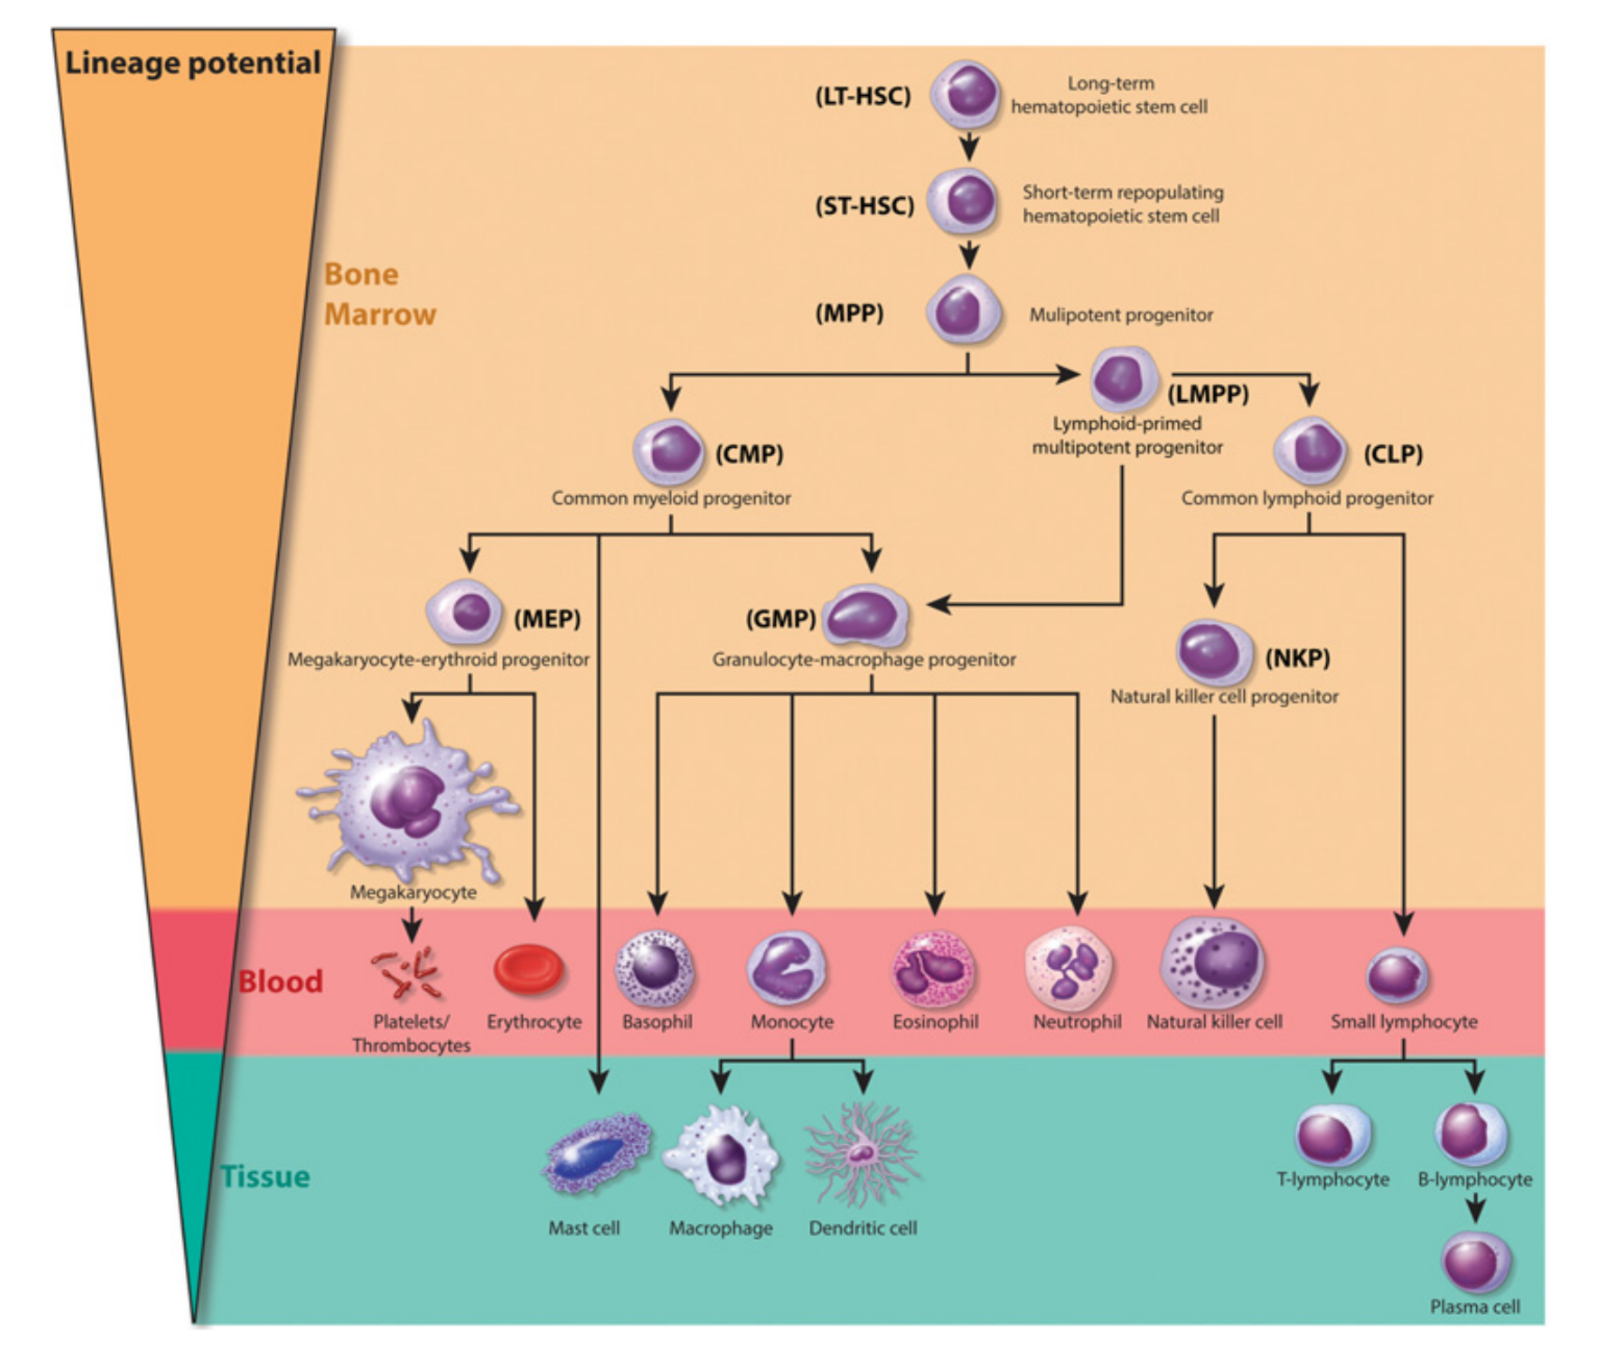
\includegraphics[width=\textwidth]{plot/ch4/hem.pdf}
  \caption[Hematopoiesis schematic]{Summary of important cell types arising during hematopoeisis from HSCs to phenotypically and functionally distinct cell types. Adapted from \textcite{Hu2016}. HSC = hematopoeitic stem cell.}
  \label{fig:hem_sum}
\end{figure}

The regulation of chromatin accessibility plays a central role in the differentiation trajectory of erythrocytes \cite{Hu2016,Schulz2019}. Erythropoesis refers to the process of  successive differentiation from pluripotent stem and progenitor cells through several morphologically and functionally distinct stages to form enucleated erythrocytes (also known as red blood cells). Here we focus on the process up until erythroblasts, the penultimate step in erythropoiesis and the last before enucleation. \textcite{Ludwig2019} used FACS sorting on CD71, CD235a, CD49d, and BAND3 surface markers to identify eight distinct stages of development. Their analysis using both ATAC-seq and RNA-seq is the most complete representation of this differentiation trajectory to date. The authors identify myloid progeneitors (MyP), colony forming units - erythroid (CFU-E), pro-erythoblasts with two stages (ProE1, ProE2), basophilic erythoblasts (Baso-E), polychromatic erythroblasts (Poly-E), orthochromatic erythoblasts (OrthoE), and orthochromatic reticulocyte (Ortho/Ret) as key cell stages. A detailed explanation of the molecular biology of each stage is not the focus of this thesis, however interested readers may consult texts such as \textcite{Sinclair2013}. After augmenting their dataset with hematopoetic progentor cells created by \textcite{Corces2016}, the authors found that accessible elements clustered into several groupings. Some were predominantly active in the earliest stages of hematopoesis, while others were broadly accessible across lineage commitment and intermediate erythropoesis, while others still acted primarily in terminal erythropoesis. 
These broad groupings allowed the authors to identify several factors of interest which may act differentially; we investigate these factors such as \textit{TMCC2, UROS}, and \textit{RHAG} as well as other well known markers like \textit{TAL1, KLF5} and \textit{GATA1} later in this chapter. In this chapter, we recreate this dataset by augmenting the eight erythroid cell type presented in \textcite{Ludwig2019} with the hematopoietic stem and progenitor cells from \textcite{Corces2016} to create a dataset of chromatin accessibility throughout erythropoesis.


\begin{figure}
  \centering
  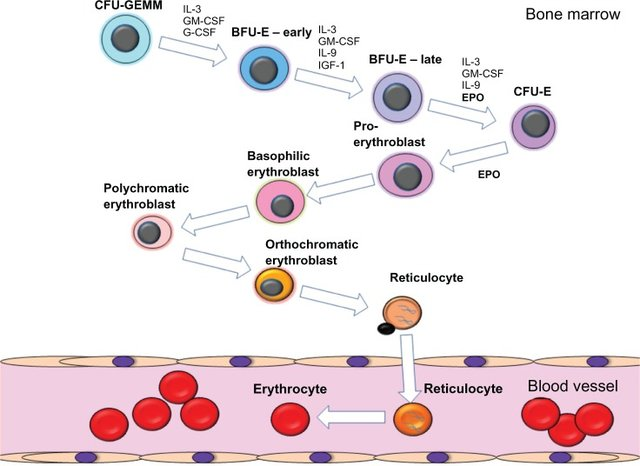
\includegraphics[width=\textwidth]{plot/ch4/ery}
  \caption[Erythropoiesis schematic]{Key stages of erythropoesis from \textcite{Sinclair2013}. Blast forming units are not represented in the \textcite{Ludwig2019} dataset, while erythroblasts replace erythrocytes as the end point of the process for our purposes.}
  \label{fig:ery}
\end{figure}





\subsection{Identifying regulatory programs in large databases}

The task of identifying co-accessible sets of regulatory elements usually falls on differential peak accessibility analyses \cite{Yan2020}. Many methods exist for this task, including MACS2, DiffBind, csaw, voom, limma, edgeR, and DESeq2 \cite{Ritchie2015,Law2014,Love2014,Robinson2009,StarkRandBrown2016,Lun2015,Zhang2008}. A comprehensive review of their relative performances was undertaken by \textcite{Reske2020}. In general, these methods work by grouping similar experiments, usually taken to be biological replicates, and finding peak regions whose deviation overcomes some level of statistical significance. These tools are highly refined and benchmarked for applications with two cell types of interest. However, using differential accessibility in large systems with multiple consistent subpopulations poses technical issues. As an example, edgeR is able to estimate coefficients for a general linear model and find significant differences in accessibility for a particular cluster. However, the estimation of statistical significance relies on estimating variance with biological replicates, and the user is warned not to attempt significance testing without performing replicates \cite{Robinson2009}. Though this places no hard constraint on the data to be analysed, clustering in large datasets is imperfect. The estimation of the variance is therefore critically reliant on the homogeneity of the cluster, which may vary between clusters. This makes the interpretation of differentially accessible elements between clusters in large datasets difficult. Secondly, it is difficult to use differential accessibility testing to find patterns unique to combinations of clusters, as the estimated coefficients tend to relate to enrichment in a specific cluster, or between all of them. One alternative is to look at the pairwise differential accessibility between clusters and search for patterns in the identified regions. This is, however, onerous and to our knowledge no dedicated method exists for the task.  

Recently, \textcite{BravoGonzalez-Blas2019} proposed the use of topic modelling to study collections of accessible regions in single cell \gls{scatac}. Topic modelling, specifically \gls{lda} represents a viable method for the unsupervised identification of key regions of accessible sequence in large databases, while simultaneously identifying the distribution of their associated regulatory programs. The method learns groupings of differentially accessible elements and where they tend to be active, in aggregate. However, the use of LDA in large collections of ATAC-seq data has not been explored. As the amount of available ATAC-seq data grows year over year, analyses of large compendiums of cellular variation in accessibility form a useful complement to sparse single cell analyses. On the one hand, single cell analyses are well powered to identify fine-scale groupings of regulatory elements active in sub populations of similar cell types. On the other, analysis of dense bulk ATAC-seq with high read depths allows for a thorough investigation of pathways active across large groupings of cells. In this chapter, we investigate the use of LDA for identifying regulatory programs and their distribution in bulk \gls{atac}.

\subsection{Latent Dirichlet Allocation}

A detailed methodological motivation of \gls{lda} is beyond the scope of this chapter, however here I present in general terms a typical formulation of the generative model and inference from real data.  

\subsubsection{The generative model}

LDA is interested in the generation of a corpus of $D$ documents, composed of $n$ words. It was introduced in \textcite{Blei2003}. In brief, each document $d = 1 \ldots D$ can be described as a collection of weights on $k$ topics. An example in the realm of natural language processing would be books and their respective genres (i.e. fiction, science, etc.). In the specific application here presented, the corpus represents the dataset of sequencing experiments, with each document representing a single ATAC-seq sample. The words are individual accessible regions, which are determined and discretized through peak calling on respective samples. The inference procedure is unsupervised, and there is no annotation or metadata given to discriminate amongst samples, unlike later adaptations like structured topic modelling \cite{Roberts2019}.

The generative process is as follows. For a fixed number of topics $k$, each document $d$ is given a distribution on its topic weights $\theta_d$ $$ \theta_d \sim Dir(\alpha), d = 1, \ldots, D $$ Each word $n$ in document $d$ is generated from a particular topic $z_{dn}$ where  $z_{dn}$ $$ z_{dn} \sim Discrete(\theta_d) $$ and the word itself is chosen from $$ p(w_{dn} | z_{dn}, \zeta) $$ which is a multinomial probability conditional on the topic allocation $z_{dn}$. The other dependency is on $\zeta$, here defined as a $k \times N$ matrix where $\zeta_{ij} = P(w_j =1 | z_i = 1)$, or the conditional probability of a word given a topic allocation. This is a fixed quantity that will be estimated. 

The Dirichlet distribution is convenient in this case, as draws from $Dir(\alpha)$ represent points on the ($k-1$) simplex where parameter $\alpha$ is a $k$-vector of positive reals. A simplex is a multidimensional generalization of the triangle. In addition, the dirichlet distribution is the conjugate prior to the multinomial distribution, a fact which is exploited for efficient inference algorithms. Explicitly, the probability density function of the Dirichlet distribution here considered is given by 

$$ p(\theta | \alpha ) = \frac{\Gamma(\sum^k_{i=1} \alpha_i)}{ \prod^k_{i=1} \Gamma(\alpha_i)} \theta_1^{\alpha_1 -1} \ldots \theta_k^{\alpha_k-1} $$ which leads to an overall joint distribution and probability of an overall corpus as given in \textcite{Blei2003}.

This traditional set up for LDA does not allow for any control over the sparsity of word allocations to topics. For that, an extension called Smoothed LDA replaces the $\zeta$ matrix of conditional word probabilities with a second Dirichlet distribution, parameterized by $\beta$. As a side note, all of the applications of LDA in this chapter are concerned with symmetric Dirichlet distributions, where each of the entries of the $\alpha$ and $\beta$ $k$-vectors are the same. This modified generative procedure proceeds identifically, except that a seperate draw is made for each topic representing the distribution on its words from $$ \psi_k \sim Dir(\beta), k = 1, \ldots, K $$, and drawing a word conditional on its topic assignment is instead generated as $$w_{dn} \sim Discrete( \psi_{z_{dn}})$$ where $\psi_{z_{dn}}$ intuitively represents the topic-word distribution. In the case here considered, it represents the importance of a particular region of accessible chromatin to a regulatory program $z$.

\subsubsection{Parameter inference}

The joint distribution of latent parameters $\theta, z$ conditional on $w, \alpha, \beta$ does not admit analytical inference as the posterior probability is intractable, as noted in \textcite{Blei2003}. They proposed an approach based on variational Bayesian inference, however it has become commonplace to integrate out $\theta$ and approach the problem of inference using collapsed Gibbs sampling \cite{Qiu2014,Magnusson2018,Park2019}. Gibbs sampling is an extension of the \gls{mcmc} approach for sampling from the posterior distribution when, as is the case here, analytical inference is not possible. Gibbs sampling is closely related to the Metropolis-Hastings algorithm, and relies on constructing a markov chain with the previously described posterior as its equilibrium distribution. In this way, inference about parameters is deduced from direct samples of the posterior. This is philosophically very similar to the approach taken in Chapter 3, where samples of the posterior distribution of geneologies conditioned on mutations were used to draw inference about demographic parameters such as directional migration. The details of the inference procedure are not of direct relevance to the results presented in this chapter, and a more detailed description can be found in \textcite{Qiu2014} and others.

Here, the posterior distribution of interest concerns the most likely values of $\theta$ and $\psi$, that is the topic weight vectors on each of the different ATAC-seq experiments and the topic distribution on each of the constituent accessible regions, conditioned on observed regions within ATAC-seq experiments and given parameters $\alpha, \beta$.

\subsection{The LDA algorithm and cisTopic}

The basis of this chapter is the cisTopic algorithm, and some expansion on its basic formulation is necessary. cisTopic is introduced in \textcite{BravoGonzalez-Blas2019}, and is primarily intended for use on \gls{scatac} data resulting from a combination of sequencing data and associated peak calls. In general, this data is either encoded in a count matrix or it is internally converted to one. A count matrix $M$, for the purposes of this chapter, refers to a $C \times R$ matrix where element $M_{cr}$ equals the number of reads (or fragments) overlapping region $r$ in cell $c$, for regions $r=1,\ldots,R$ and cells $c=1,\ldots,C$. Each region $r$ is selected on the basis of statistical peak calls, typically performed with software such as Macs2 or similar, on the aggregated \gls{scatac} signal. This count matrix $M$ is then subjected to binarisation on the basis of some threshold $T$, where $T$ is the minimum number of counts necessary for a region to be declared accessible. This threshold reflects the low sequencing depth of \gls{scatac} data, and the difficulty in comparing cells quantitatively based on read counts alone without some correction for depth. This threshold is set to 1 by default in the stable version of the algorithm implementation.

The corrected count matrix is used for the inference of the cell-topic distribution and the region-topic distribution, previously represented by $\theta$ and $\psi$ respectively as the distribution of topics over documents and the distribution of words over topics. Topic loadings for both the cell and region loadings are normalized to the range [0, 1]. Key regions which are important to the topic may be selected in one of two ways. Firstly, by fitting a gamma distribution to the normalized region-topic loadings on a per-topic basis and selecting a percent point threshold of the resulting density's tail (i.e. the top 1 percentile of the fit gamma distribution). Alternatively, a given number of top regions may be selected based on the rank of the region-topic loadings.  

Selecting the right number of topics for a particular analysis is not straight forward. cisTopic implements an optimized version of collapsed Gibbs sampling by using WarpLDA, an algorithm for constant time inference \cite{Chen2016a}. An advantage of warpLDA is that it returns the second derivative of each value for $k$. As loglikelihood values increase with increasing $k$, cisTopic makes use of these values to automatically select a value for $k$ based on a range given by the user. A proof that this procedure produces optimal values of $k$ is not readily available. 

\subsection{Aims of this chapter}

The overarching aim of this chapter is to investigate the use of LDA for bulk \gls{atac}. As noted above, the method represents a significant advancement above differential accessibility, and shows theoretical promise for the analysis of the growing collections of sequencing data in diverse cell systems. In doing so, I adapt the existing cisTopic method for bulk samples. Specifically, I investigate the performance of bulk LDA when compared to established \gls{scatac} inference using cisTopic. I also investigate whether the method infers meaningful topic loadings on a well understood system with ground truth values to compare against, erythopoiesis.   

% What is the goal. 
%   Identify important discriminatory regulatory elements and how they are shared amongst groups of cells. 
% Why LDA?
%   differential peak analysis can decide a statistical threshold for two different cell types.
%   there are many different methods for DA analyses MACS2, DiffBind, csaw, voom, limma, edgeR, and DESeq2 [27,28,29,30,31,32,33]
%   it is sensitive to the normalisation and data processing, given how these interact with the statistic model of choice (https://epigeneticsandchromatin.biomedcentral.com/articles/10.1186/s13072-020-00342-y)
%   Impractical to perform pairwise comparisons and attempt to infer patterns in this by eye.
%   Some approaches exist to look at pathways of cells (citation here??? ) during differentation. However, the problem of identifying both common and discriminatory regulatory elements remains open. 
%   Recently LDA has been proposed to look at the accessibility of dna in single cell atac-seq.

%   Advantages:
%     no assumption that a region is important only to a certain cell type or topic. A single region can contribute to many different topics, in different contexts.
%     consider groupings of elements as important, gives annotation to grouops of regions more so than answering the question of "what it different", it is answering, what is important 

%   Disadvantages:
%     Bag of words assumes no direct interaction betewen regions. Though there is biological rationale to consider how regions interact with each other, it is difficult to formulate this beyond co-occurance.

% Discussion should include somethign about there being more comprehensive models of topic modelling like structured topic modelling (stm package and https://cbail.github.io/SICSS_Topic_Modeling.html)

\section{Methods} \label{ch4:methods}


\subsection{Single Cell ATAC-seq Dataset Generation} \label{methods:sc_ds}

A single cell ATAC-seq dataset was compiled from data generated in \textcite{Buenrostro2015} for three cell types: K562, GM12878, and H1ESC. These cell types were selected as a subset which represents maximal diversity in accessible chromatin within the larger dataset. 

For each labelled cell type, we collected accession numbers within the NCBI sequence read archive. These include records SRR1780163 through SRR1780354 (K562), SRR1779683 through SRR1779778 (GM12878), and SRR1779589 through SRR1779683 (H1ESC). Sequencing reads were merged and adapters were trimmed with cutadapt v 2.10 using the following adapter seqences ({\tt -a CTGTCTCTTATACACATCT -A CTGTCTCTTATACACATCT}) \cite{Martin2011}. Quality of the merged dataset was verified with fastqc and aligned to hg19 using bowtie2 \cite{Andrews2010, Langmead2013}. Cell specific barcodes were added to the resulting alignment file within the {\tt CB} tag using pySam \cite{Heger2009}. Peak calling was performed using MACS2 and LanceOTron using default parameters \cite{Gaspar2018, Hentges2021} as detailed in \autoref{ch4:method_peaks} and count matrices were constructed as detailed in \autoref{ch4:method_cistopic}. A more thorough discussion of our choice to compare MACS2 and LanceOTron may be found in \Cref{intro:pc}.

\subsection{Construction of Pseudo-bulk ATAC-seq Dataset}

In order to construct a pseudo-bulk dataset, entries for each of the single cells were merged into a single alignment file. Cell barcodes were replaced with a cell-type marker and peak calling was similarly conducted with macs2 and lanceotron \cite{Gaspar2018, Hentges2021}.

\subsection{Peak Calling from Coverage Data} \label{ch4:method_peaks}

We compare two methods of peak calling.

A public implementation of the LanceOTron can be found at \url{https://github.com/chris1221/lanceotron}. LanceOTRon relies on a pre-trained neural network. We use the supplied weights in \url{wide_and_deep_fully_trained_v5_03.h5} along with the standard scaler values from the same implementation. We allow the network to identify candidate peaks and assign a peak score, thresholding our selected peaks on a peak score of at least 0.5 as in the implemention of LanceOTron at \url{https://lanceotron.molbiol.ox.ac.uk/}.


\subsection{Running LDA with cisTopic} \label{ch4:method_cistopic}

We used the implementation of \gls{lda} in cisTopic \cite{BravoGonzalez-Blas2019}. cisTopic is intended for use on single cell ATAC-seq experiments, however the input format is amenable to any quantitative data observed on a cell by region basis. To construct the input data to cisTopic, we create a bespoke pipeline that firstly calls peaks from ATAC-seq experiments, and secondly harmonizes these peaks while constructing a count matrix. A count matrix is a sparse matrix where the rows are cells, or in the case of this thesis, cell types in the form of ATAC-seq samples, and the columns are individual peak regions.

\subsection{Bayesian Hyper-parameter Optimization} \label{ch4:hyper}

\gls{lda} requires a set of three hyper-parameters to be supplied, alpha, beta, and the number of topics. This chapter investigates applications of LDA to problems of several scales, so the choice of hyper-parameters is not easily chosen, at least in an unbiased way. We approach this issue by using a Bayesian Optimization approach to learn the best set of hyper parameters for a given set of ATAC-seq experiments. We wrote a typical cisTopic analysis in python via rpy2 ({\tt https://rpy2.github.io/doc/latest/html/index.html}) and used the BayesianOptimization library ({\tt https://github.com/fmfn/BayesianOptimization}) to optimize a target function for a given set of hyper-parameters. This task was facilitated by the use of Dask to compute several hundred possible combinations simultaneously \cite{Rocklin2015}. The target function to optimise is based on the specific application, as discussed in \autoref{ch4:results} section.

\subsection{Bulk LDA (BLDA) Method} \label{ch4:method_blda}

The BLDA method is a small extension to cisTopic which aims to incorporate a proxy of how accessible each peak region is in a particular experiment. This makes it in some ways more similar to the traditional approach to LDA within natural language processing, which gives an integer value for the number of times a particular word appears in a text. To create the RPKM normalized count matrix and run the inference, we use functions from the blda python package available on Github at \url{https://github.com/Chris1221/blda}. \todo{Link the snakemake pipeline minus the data.} The construction of the count matrix requires linked coverage files and their associated peak calls. The pipeline is agnostic to the type of coverage file (either BAM files or RPKM normalised bigWig tracks can be provided) and peak calls can be made by any software which outputs delineated, non-overlapping genomic regions. Hyper-parameter optimization is conducted according to \Cref{ch4:hyper} and a modified version of cisTopic is run using {\tt rpy2}. The modification to cisTopic, found at \url{https://github.com/Chris1221/cisTopic}, relaxes a constraint to provide the {\tt lda} package's collapsed Gibb's sampler with a binary sparse matrix. Several other functions from the cisTopic function are applicable directly to the situation of bulk LDA after the data has been altered. 

\subsection{Computing the average fold enrichment of topics for groups} \label{methods:average_fc}

To get a measure for the number of topics to use in a particular model, we compute the average fold enrichment. This is done with a two step process. First, a one-tailed student's T test is performed for each of the grouping of cells. The cells are split into one of the cell types, with the remainder forming the comparison group. The null hypothesis here is that the means do not differ, or that the comparison group is significantly smaller than the group under question. The P values are corrected for the number of comparisons using Bonferroni correction (multiplying by the number of effective tests, which in this case is the number of tests) and the significant associations are reported. Second, the differences in the estimated means are divided to form a fold change metric amongst the subset of significant topic associations. We take the median of these values to form the average fold change metric for a particular set of topics being modelled. The median is selected to avoid extreme results overly biasing the statistic.

\subsection{Coenrichment of topics}

The number of times two topics $i$ and $j$ are co-enriched is defined to be the count of occurrences where a single cell type has a topic loading for $i$ and $j$ exceeding some pre-defined threshold. After some experimentation, we decide to use a threshold of 0.25, where the two co-enriched topics collectively form half of the normalised topic-loadings. 

\section{Results} \label{ch4:results}

LDA has previously been shown to be highly effective at detecting true patterns in shared accessibility in single cell data. Here, I create a datset of known cell types in order to set baseline expectations about the capabilities of LDA in a single cell system before moving on to studying bulk samples.

\subsection{Bulk LDA recapitulates patterns from single cell ATAC-seq}

I generated a dataset of three labelled cell types, as per \Cref{methods:sc_ds}. This dataset comprises three cell types which have substantial differences in their accessible DNA.  K562 is an erythro-leukemic cell model of chronic myelogenous leukemia from a fifty three year old female donor \cite{Lozzio1975}. GM12878 is an \gls{ebv} immortalized B-lymphocyte cell line cultured from a female member of the international HapMap project CEPH panel \cite{Belmont2005}. Finally, H1ESC are a human embryonic stem cell line collected from a healthy male donor of unknown age \cite{Thomson1998}. 

The dataset comprises 96 GM12878 cells with a total of 1928090 reads, 96 H1ESC cells with 4192100 reads in total, and 192 K562 cells from two biological replicates with a total of 5269388 reads.

We generate coverage tracks for the merged single cell dataset using deepTools and peaks are called using both MACS2 and LanceOTron as per \Cref{ch4:method_peaks} \cite{Ramirez2014}. MACS2 identifies 10,075 statistically significant peak regions, while MACS2 finds 12,994, 8337 of which are common between the two approaches.  

\subsubsection{Identifying differentially accessible peaks with EdgeR} \label{ch4:edgeR}

The R package {\tt edgeR} is used to set a baseline expectation for differentially accessible regions of the genome between the clusters. {\tt edgeR} is selected as it was recently shown to have the overall highest sensitivity for identifying differential peaks from properly normalized ATAC-seq data. We took the single cell dataset and created a count matrix with all true counts across different cells. We inputted these into edgeR and estimated dispersion coefficients as recommended in the tutorial, fitting a generalised linear model according to the true cell identities which assume are known in this case. We identify the top 100 differentially accessible regions based on this analysis, and use these to study the results from our topic modelling approaches.

\begin{figure}
  \centering
  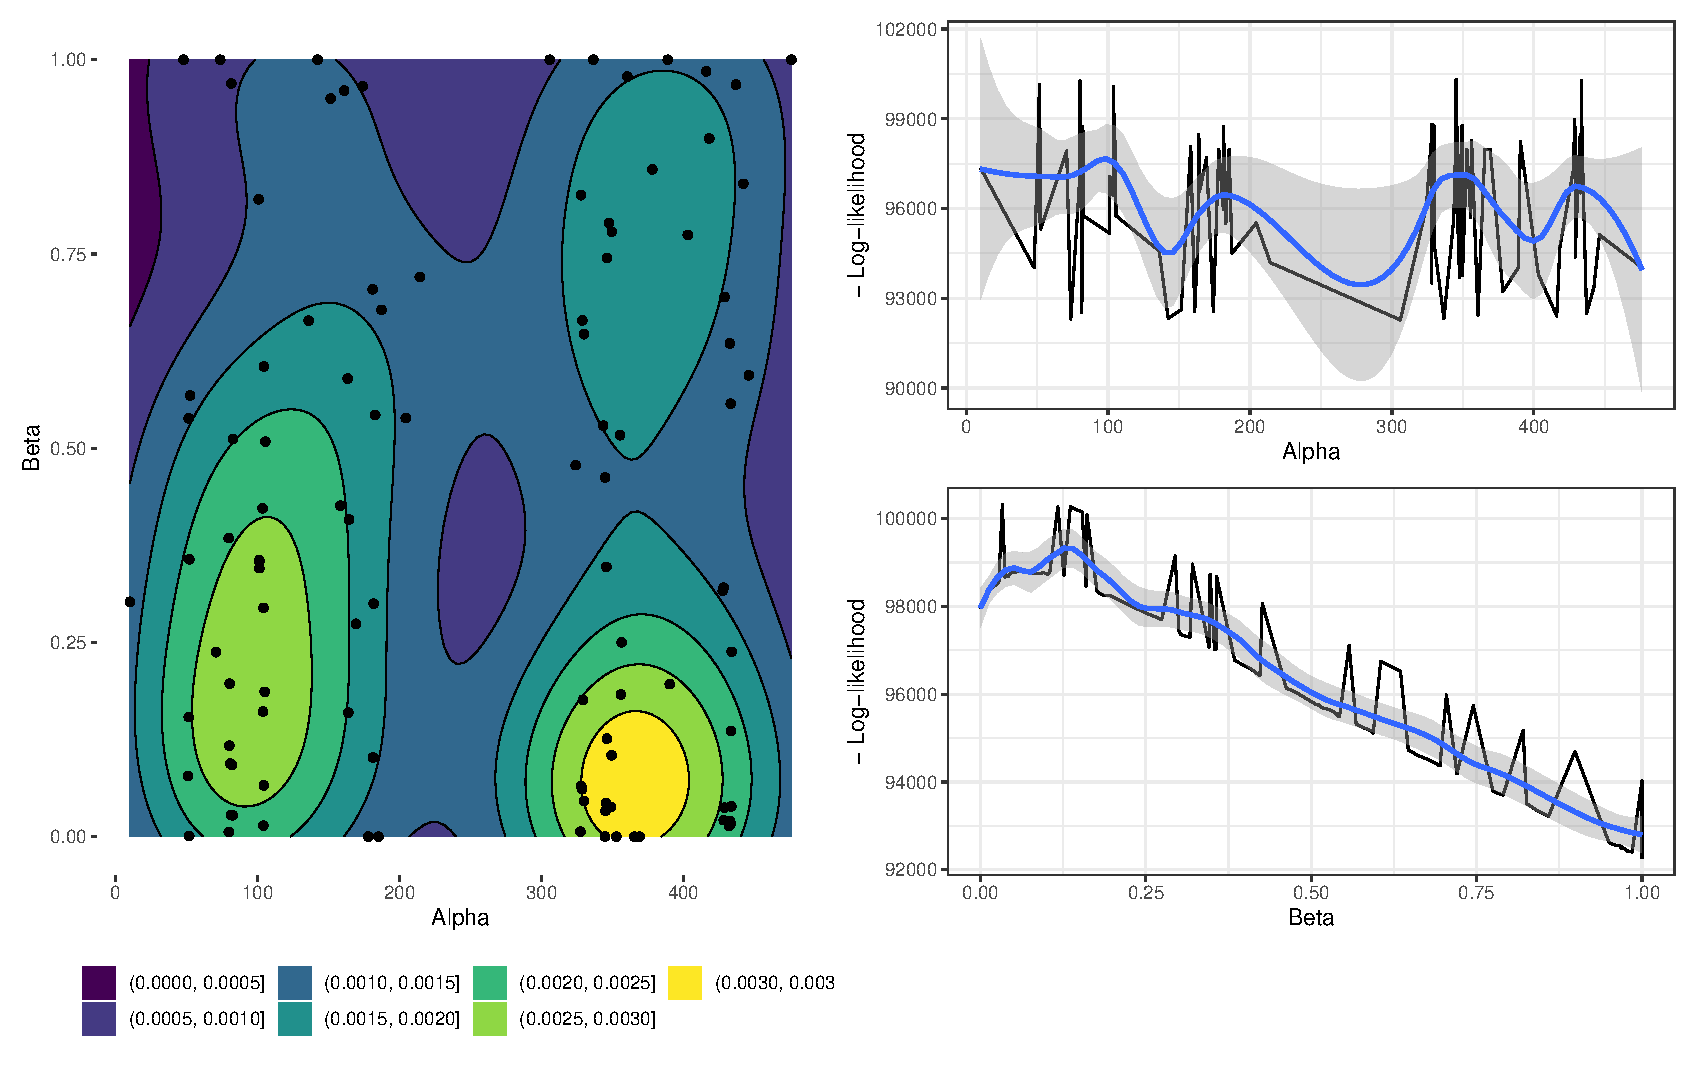
\includegraphics[width=\textwidth]{plot/ch4/sim_ll_surface.pdf}
  \caption{Hyperparameter log-likelihood surface for two hyperparameters.}
  \label{fig:llhood_surfacea_simulation}
\end{figure}

We investigate topic modelling in three separate scenarios. Firstly, we run cisTopic as intended, using the single cell data. Secondly, we create pseudo-bulk alignment files for each of the clusters and run cisTopic normally. Thirdly, we adapt cisTopic to accept normalized read count. This will allow us to validate our baseline assumption that LDA is able to capture similar information within bulk sequencing experiments.

\subsubsection{LDA captures realistic regulatory patterns in known single cell systems} \label{ch4:sc}

For the first case, we model the system of 384 cells with 4, 5, 6, 7, and 8 topics to assess the best biological fit to the system. For each pre-set number of topics, hyper parameters are selected using Bayesian optimization. The best value for $\alpha$ was not well estimated, with considerable noise and no clear peak; this is in contrast to the $\beta$ value, which showed higher log-likelihoods at higher values approaching 1 (\Cref{fig:sc_opt_params}). Consistent with this, a high value is selected for $\beta$ in each case. $\beta$ controls the number of regions loaded to a topic. With a number of cells much larger than the number of topics, especially in the present scenario, a high value of $\beta$ represents a prior on more regions loaded to each of the small number of topics. This indicates that a relatively high number of regions are differentially accessible between the different clusters. The relatively uncertain distribution of alpha log-likelihoods represents an ambiguity in the likelihood from different Dirichlet distributions. Draws with a low alpha tend to represent topic loadings which are specific to individual cells, and accordingly the flat likelihood surface may indicate that there are multiple ways of assigning the topics to cells with relatively equal likelihoods.

\todo{The alpha is off on \Cref{fig:sc_topics}, and I want to add labels to the K562 versus H1ESC and GM cells.}

\begin{figure}
  \centering
  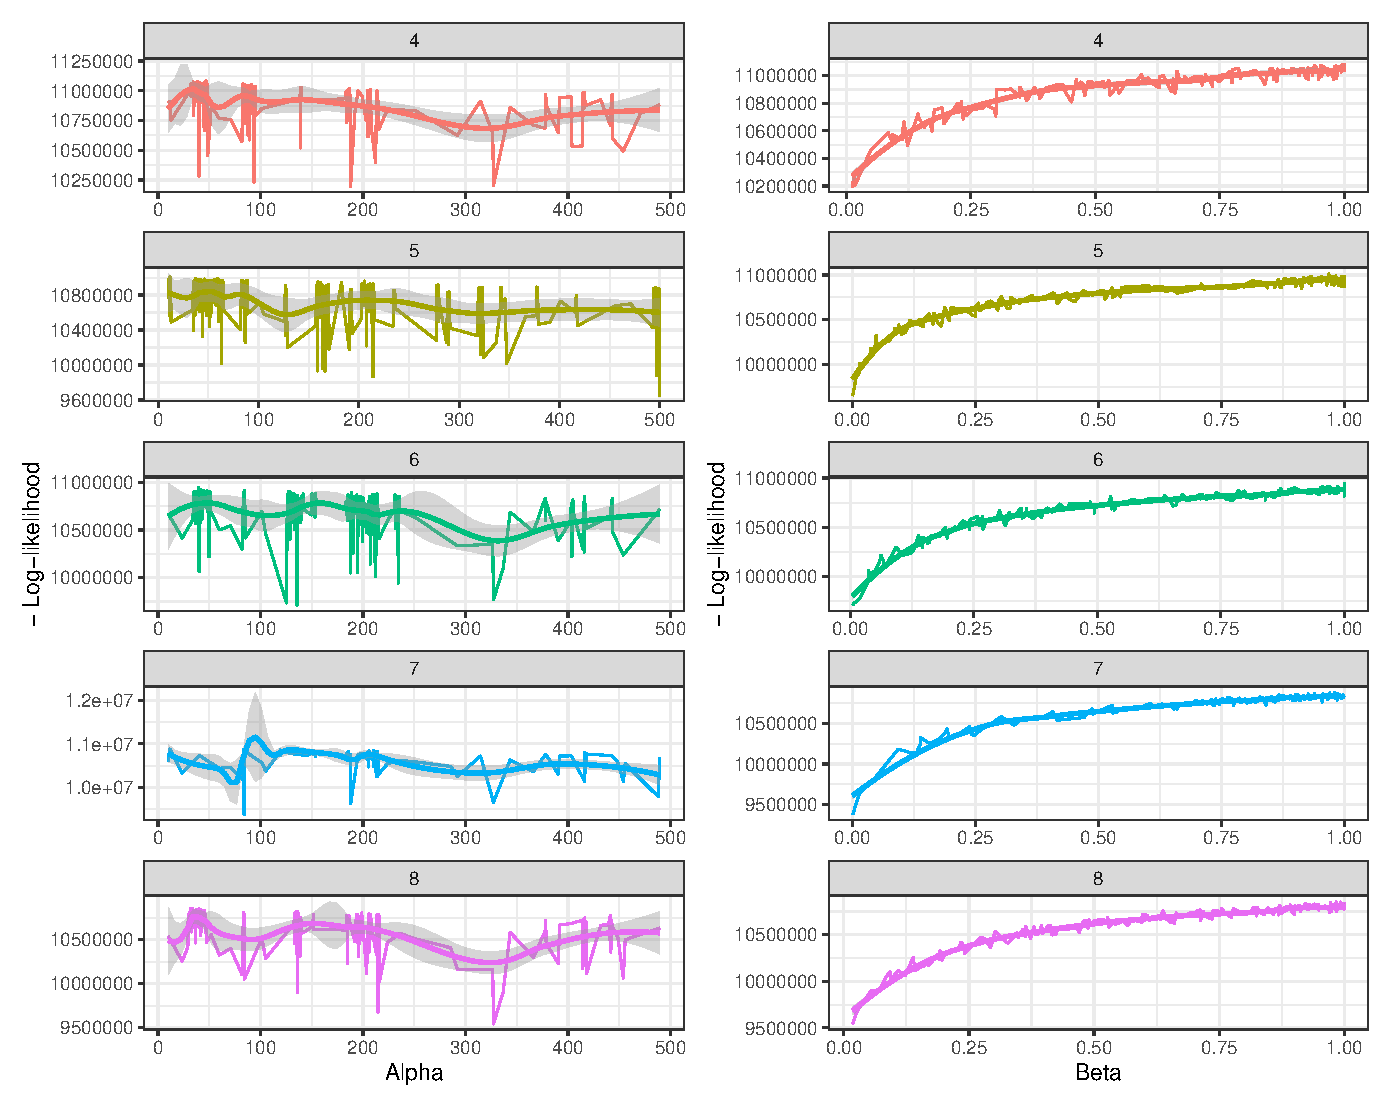
\includegraphics[width=\textwidth]{plot/ch4/sc_opt_params}
  \caption{Single cell log likelihood for different values of the topic modelling hyper-parameters $\alpha$ and $\beta$ for various numbers of topics being modelled.}
  \label{fig:sc_opt_params}
\end{figure}

We investigate the loading of these topics on each of the cells in the collection (\Cref{fig:sc_topics}). As the number of topics modelled increases, some cell systems split more readily than others. H1ESC, for instance, has two enriched topics in even the smallest four topic model. For each of the number of topics, we calculate the median fold enrichment (\Cref{methods:average_fc}) and find that five and six topics produce very similar median fold enrichments (5.81 versus 5.82 respectively). To reduce the complexity of the model, and acknowledging that a model with more parameters will tend to fit data better, we choose the study the case with five topics.  

\begin{figure}
  \centering
  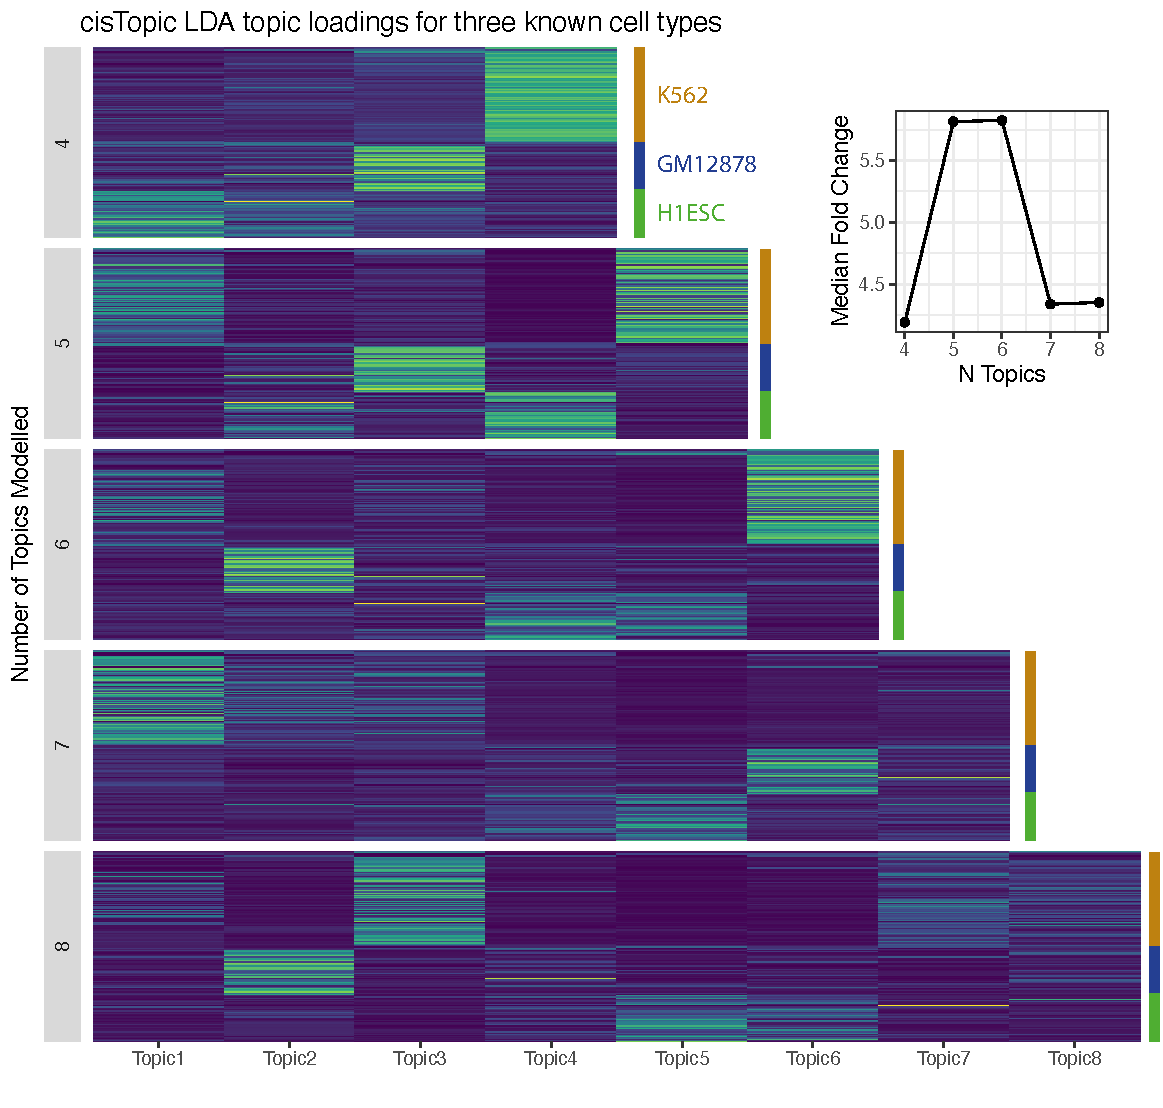
\includegraphics[width=\textwidth]{plot/ch4/sc_topics.pdf}
  \caption{Topic loadings for 4, 5, 6, 7, and 8 topic instances of the LDA inference procedure using optimal hyperparamters as decided in \Cref{fig:sc_opt_params}. Inset shows average fold change amungst enriched topics for each of the number of topics modelled. Enriched topics are identified by a one-tailed student's $t$ test for difference between a known cell cluster and the remainder of cells.} 
  \label{fig:sc_topics}
\end{figure}

\paragraph{Choice of peak caller influences the inference of topic loadings}

We additionally investigate the role that peak calling has on the inference of topics. 

Peaks were called with Macs2 instead of LanceOTRon, resulting in a larger number of peaks identified in general, with 4657 being uniquely identified by Macs2 (\Cref{fig:sc_macs2}A). We repeated the above analysis, including the hyper parameter search, topic inference, and calculation of median fold enrichment was conducted using MACS2 instead of LanceOTron, as detailed in \Cref{ch4:method_peaks}. Several differences are apparent in both the optimized hyper-parameters and the inferred topic loadings (\Cref{fig:sc_macs2}). Slight bias towards lower $\alpha$ values is observed in this dataset, and the same trend towards prefering higher values of $\beta$ is replicated here \Cref{fig:sc_macs2}B, C. However, when looking at the inferred topics, we find lower median fold enrichment in general (\Cref{fig:sc_macs2}D, E). From this we conclude that LanceOTron has identified a more specific set of accessible regions for the purposes of this study, and use it in all analyses going forward. 

\begin{figure}
  \centering
  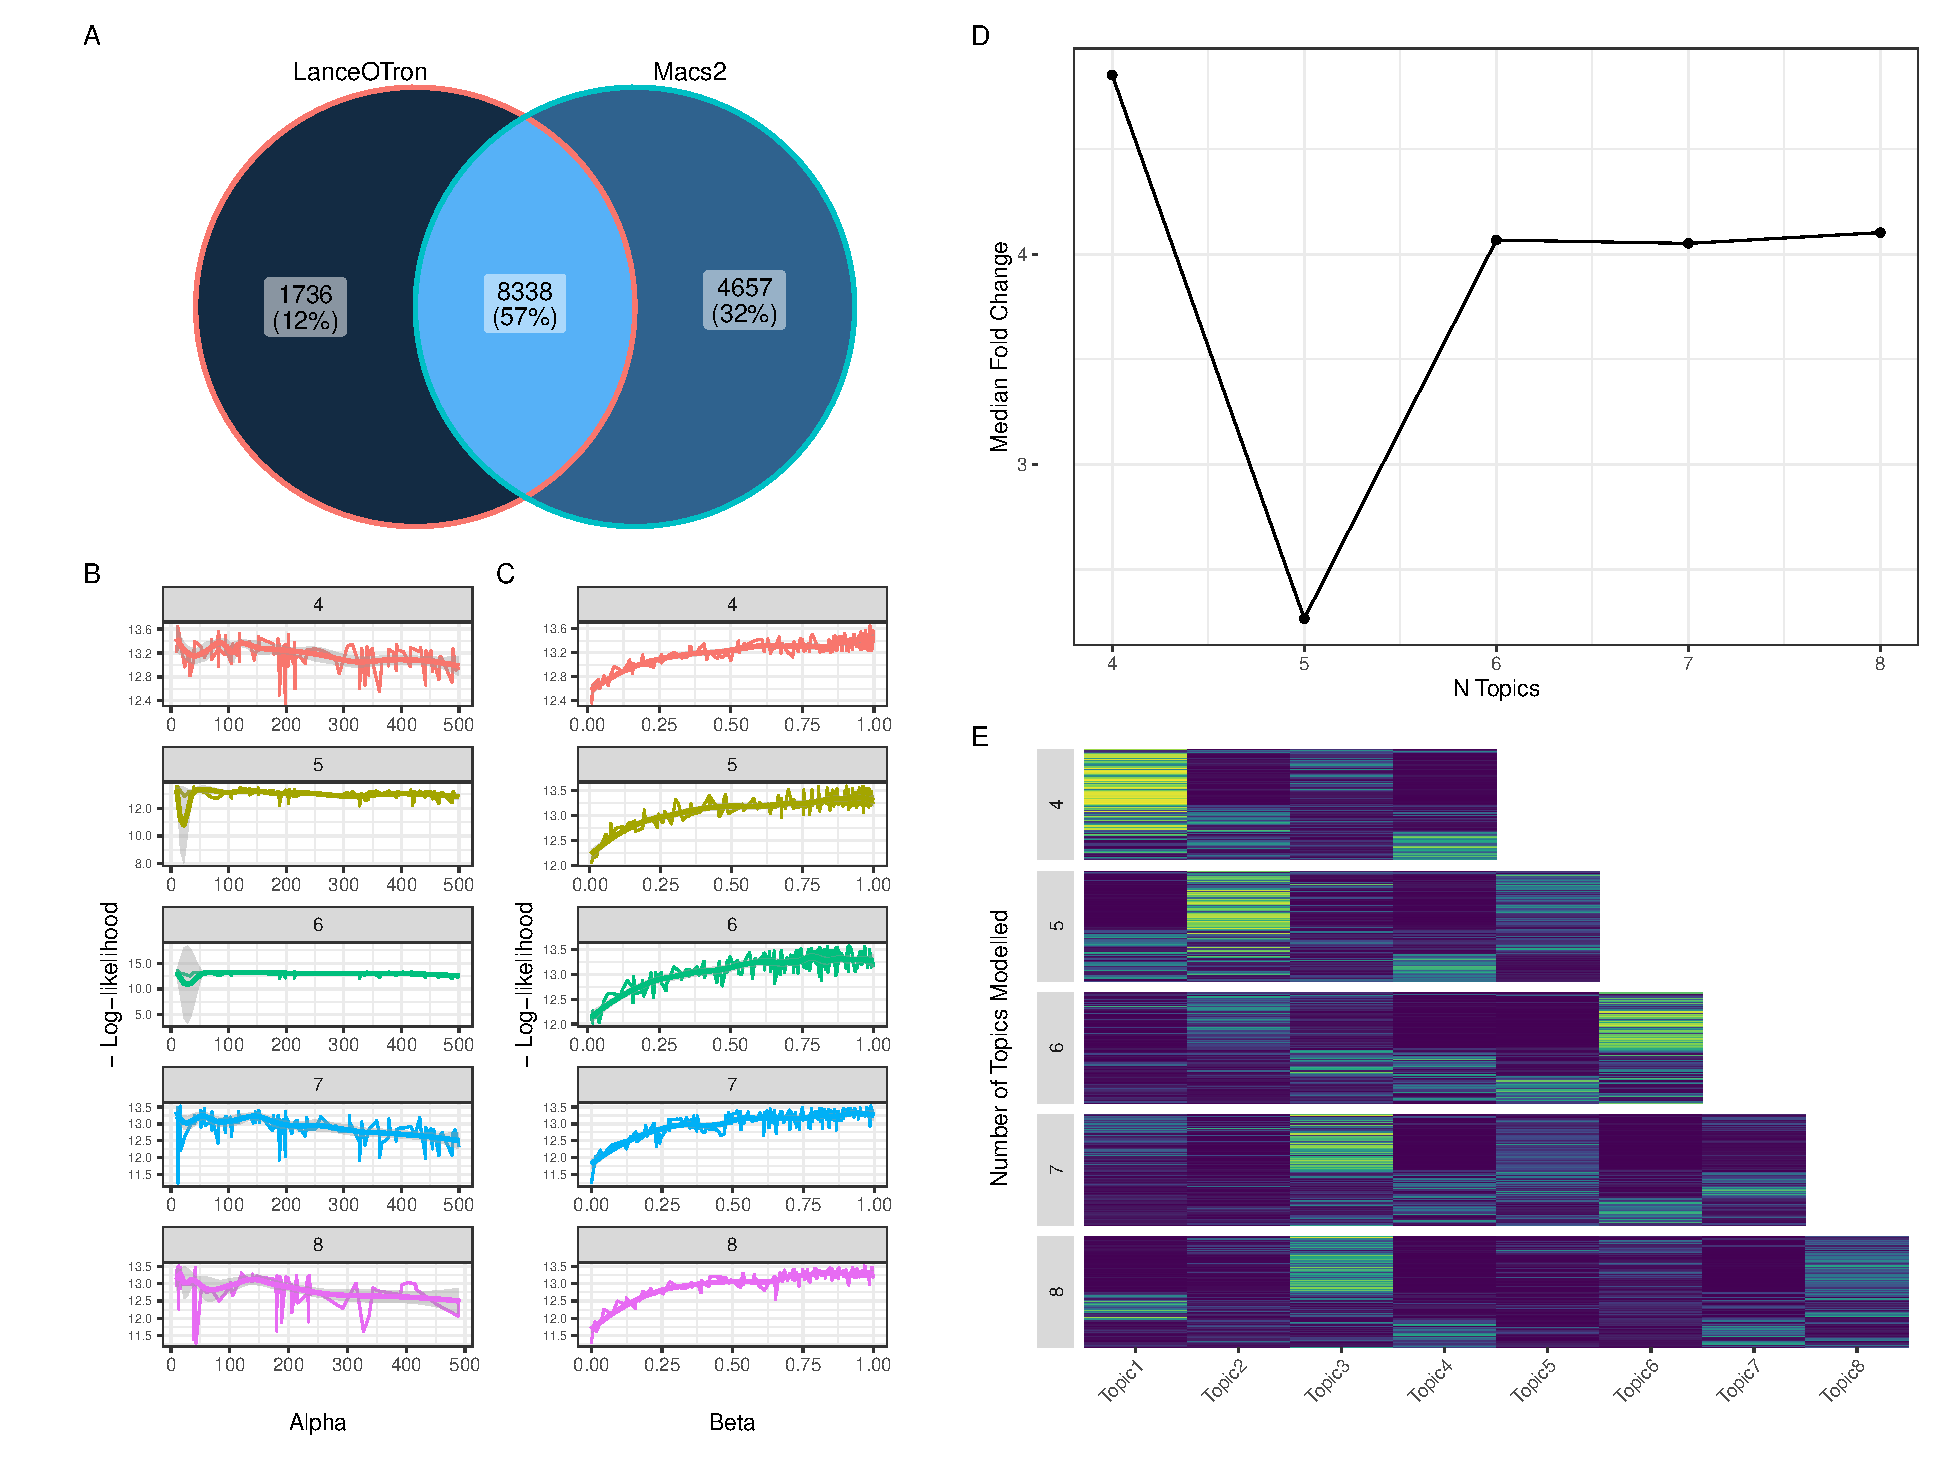
\includegraphics[width=\textwidth]{plot/ch4/sc_macs2.pdf}
  \caption{Analysis of single cell dataset with peaks called by MACS2. A. The number of peak calls made by both callers, with their overlapping portion displayed in the center of the Venn diagram. B. Likelihood surface for the optimization of the $\alpha$ hyper-parameter. C. Likelihood surface for the optimization of the $\beta$ hyper-parameter. D. Median fold enrichment for topics inferred under optimal hyper-parameters. E. Inferred topic loadings on single cells using optimal hyper-parameters.}
  \label{fig:sc_macs2}
\end{figure}

LDA produces both a distribution of topic loadings on cells as well as topic loadings on regions. In order to identify regions putatively identified with the cell types through the topic loadings, a decision must be made about how to discretise the continuous loadings to a set of enriched regions. The cisTopic package accomplishes this by fitting a gamma distribution to the topic loadings, and identifying regions within the top user-defined percentile of this distribution. By default, this is set to the top 5\% of the distribution. Here we investigate how to set this parameter value and the influence it has on the resulting post-hoc analyses. 


\todo{Motif analysis here. Feather databse is still downloading so wait for it.}

\paragraph{Enrichment of differentially accessible regions within identified topics}

To assess whether the identified topic loadings represent similar trends to the baseline differential accessibility analysis, we fit a gamma distribution to the shape of each topic loading and take the top 2.5 percentile of the distribution as representative so-called "keywords" or key regions. We use bedtools to overlap these key regions with the 100 differentially accessible regions from the {\tt edgeR} analysis and find that 61 of the 100 regions are shared with the top 415 selected key regions (\Cref{table:sc_t5_over}). Given that there are 10074 regions in total, this represents a significant ($P<0.00001$, $\chi^2 = 827.33$) enrichment of differentially expressed regions in the selected regions from the LDA procedure.


\begin{table}
  \centering
  \begin{tabular}{l|l|l}
  Topic & Total Selected Regions & Intersecting Regions  \\ 
  \hline
  1     & 104                    & 15                    \\
  2     & 3                      & 0                     \\
  3     & 194                    & 29                    \\
  4     & 3                      & 1                     \\
  5     & 111                    & 19                   
  \end{tabular}
  \caption{Five topic single cell inferred topic loadings and the proportion of their selected regions which overlap 100 established differentially accessible regions. Overall, 61 of the 100 regions were found in the top 415 regions.}
  \label{table:sc_t5_over}
  \end{table}

\subsubsection{Extending LDA to Pseudo-bulked Single Cells}

We investigate whether the approach implemented in cisTopic is appropriate for use in bulk ATAC-seq experiments. This change represents a deviation in the intended system for the approach. Practically, the difference between the single cell case and the bulk one is the difference between a wide, sparse count matrix and a dense one with fewer observations. An attractive property of using Gibb's sampling to infer the posterior cell-topic distribution is its ability to efficiently deal with sparsity in the region-topic distribution. However, it is not clear to what degree this sparsity is a requirement for the procedure to obtain biologically relevant topics, each representing a proxy of co-accessible regulatory elements. In this section, I take the well-characterized single cell dataset from the previous section and study the analogous bulk sequencing case by artificially creating bulk samples from the individual known cell types. We denote these new bulk cells as pseudobulked samples.

We combine all reads from each known cell type into pseudo-bulked alignment files using pySam. Peak calling is performed separately on each of the pseudo-bulked samples using LanceOTron, as described in the single cell case. We additionally explore the role of thresholding on LanceOTRon peak calls by creating a subset of calls with at least 0.5 peak score. This is a recommendation made by the web interface to the peak caller. Before thresholding, 517620, 395953, and 455886 peaks were identified in the H1ESC, GM12878, and K562 cells respectively. After merging, 1063153 regions were used for the complete analysis. After thresholding on a peak score of 0.5, 7524, 4945, and 6722 peaks were found in the GM12878, H1ESC and K562 cells respectively. After merging, there were 16210 regions in total used for the thresholded case. 

We take two approaches to constructing the count matrix. The first is the already described cisTopic method, where peak regions are merged and annotated by contributing cell types, leading to a binary sparse matrix where the entries $i, j$ represent overlapped peak $j$ in cell type $i$. We denote this case as "one-hot encoded" as the representation is analogous to one-hot encoding factor levels within a design matrix. This approach is justified with the single cell case as read depth is much lower per cell, and a quantification of relative read support for a particular peak region is highly variable. In the case of bulk ATAC-seq however, a difference in read support for different regions can imply varying degrees of accessibility, a key feature of closely related cell types or differentiation processes.  \todo{CITE THIS} To reflect this in the model, we propose an extension of the cisTopic method which we call bulk LDA (BLDA). In this extension, we normalize read counts according to the floor of their reads per kilobase pair and million reads (RPKM) normalized value, giving an integer value of effective number of times the "word", or region, is represented in the particular dataset. This approach has the advantage of incorporating quantitative information about differential peak strengths across experiments, and more closely mimics typical applications of LDA within natural language processing. Here we investigate whether the quantitative extension of cisTopic for bulk ATAC-seq is able to better recapitulate the single cell case.

\begin{table}
  \centering
  \begin{tabular}[t]{lrrr}
  \toprule
  Method & Number of topics & Best Alpha & Best Beta\\
  \midrule
  \cellcolor{gray!6}{One-hot encoding} & \cellcolor{gray!6}{4} & \cellcolor{gray!6}{123.68822} & \cellcolor{gray!6}{0.0382351}\\
  One-hot encoding & 5 & 466.58752 & 0.0665157\\
  \cellcolor{gray!6}{One-hot encoding} & \cellcolor{gray!6}{6} & \cellcolor{gray!6}{450.96735} & \cellcolor{gray!6}{0.0756824}\\
  One-hot encoding & 7 & 337.58572 & 0.0769945\\
  \cellcolor{gray!6}{One-hot encoding} & \cellcolor{gray!6}{8} & \cellcolor{gray!6}{100.35205} & \cellcolor{gray!6}{0.0872716}\\
  \addlinespace
  RPKM Normalization & 4 & 40.38505 & 0.2350854\\
  \cellcolor{gray!6}{RPKM Normalization} & \cellcolor{gray!6}{5} & \cellcolor{gray!6}{285.51986} & \cellcolor{gray!6}{0.3011584}\\
  RPKM Normalization & 6 & 285.70995 & 0.4163319\\
  \cellcolor{gray!6}{RPKM Normalization} & \cellcolor{gray!6}{7} & \cellcolor{gray!6}{366.02309} & \cellcolor{gray!6}{0.3825605}\\
  RPKM Normalization & 8 & 101.26750 & 0.3455916\\
  \bottomrule
  \end{tabular}
  \caption{Optimal LDA hyper-parameters for pseudo-bulked scATAC-seq parameterized by \textit{a priori} defined topic numbers and two different read quantification methods.}
  \label{table:pb_opt_params}
\end{table}

We decided hyper-parameters through Bayesian Optimization with four through eight topics, the same as the single cell case for consistency for both approaches separately. We have omitted the likelihood surfaces and provided the optimal parameters after 500 iterations in \Cref{table:pb_opt_params}. We run classic LDA for the \gls{ohe} and our extended BLDA cases using the selected hyper-parameters and compare the inferred topic loadings between the approaches (\Cref{fig:pb_no_thresh_lot_topics}). Given the small number of dense cells which share a high proportion of peak regions, in both the entire peak dataset and the thresholded one the BLDA method produces sharper and more defined topic loadings onto the individual pseudo-bulk cells. The cell-topic distribution is not noticeably different between the thresholded and non-thresholded peak calls (A versus B, \Cref{fig:pb_no_thresh_lot_topics}).
The OHE case for this data was unable to produce topics which differentiated between the difference cell types, while the RPKM normalization may have allowed the inference procedure to select regions which varied in their accessibility (left versus right, \Cref{fig:pb_no_thresh_lot_topics}). 

\begin{figure}
  \centering
  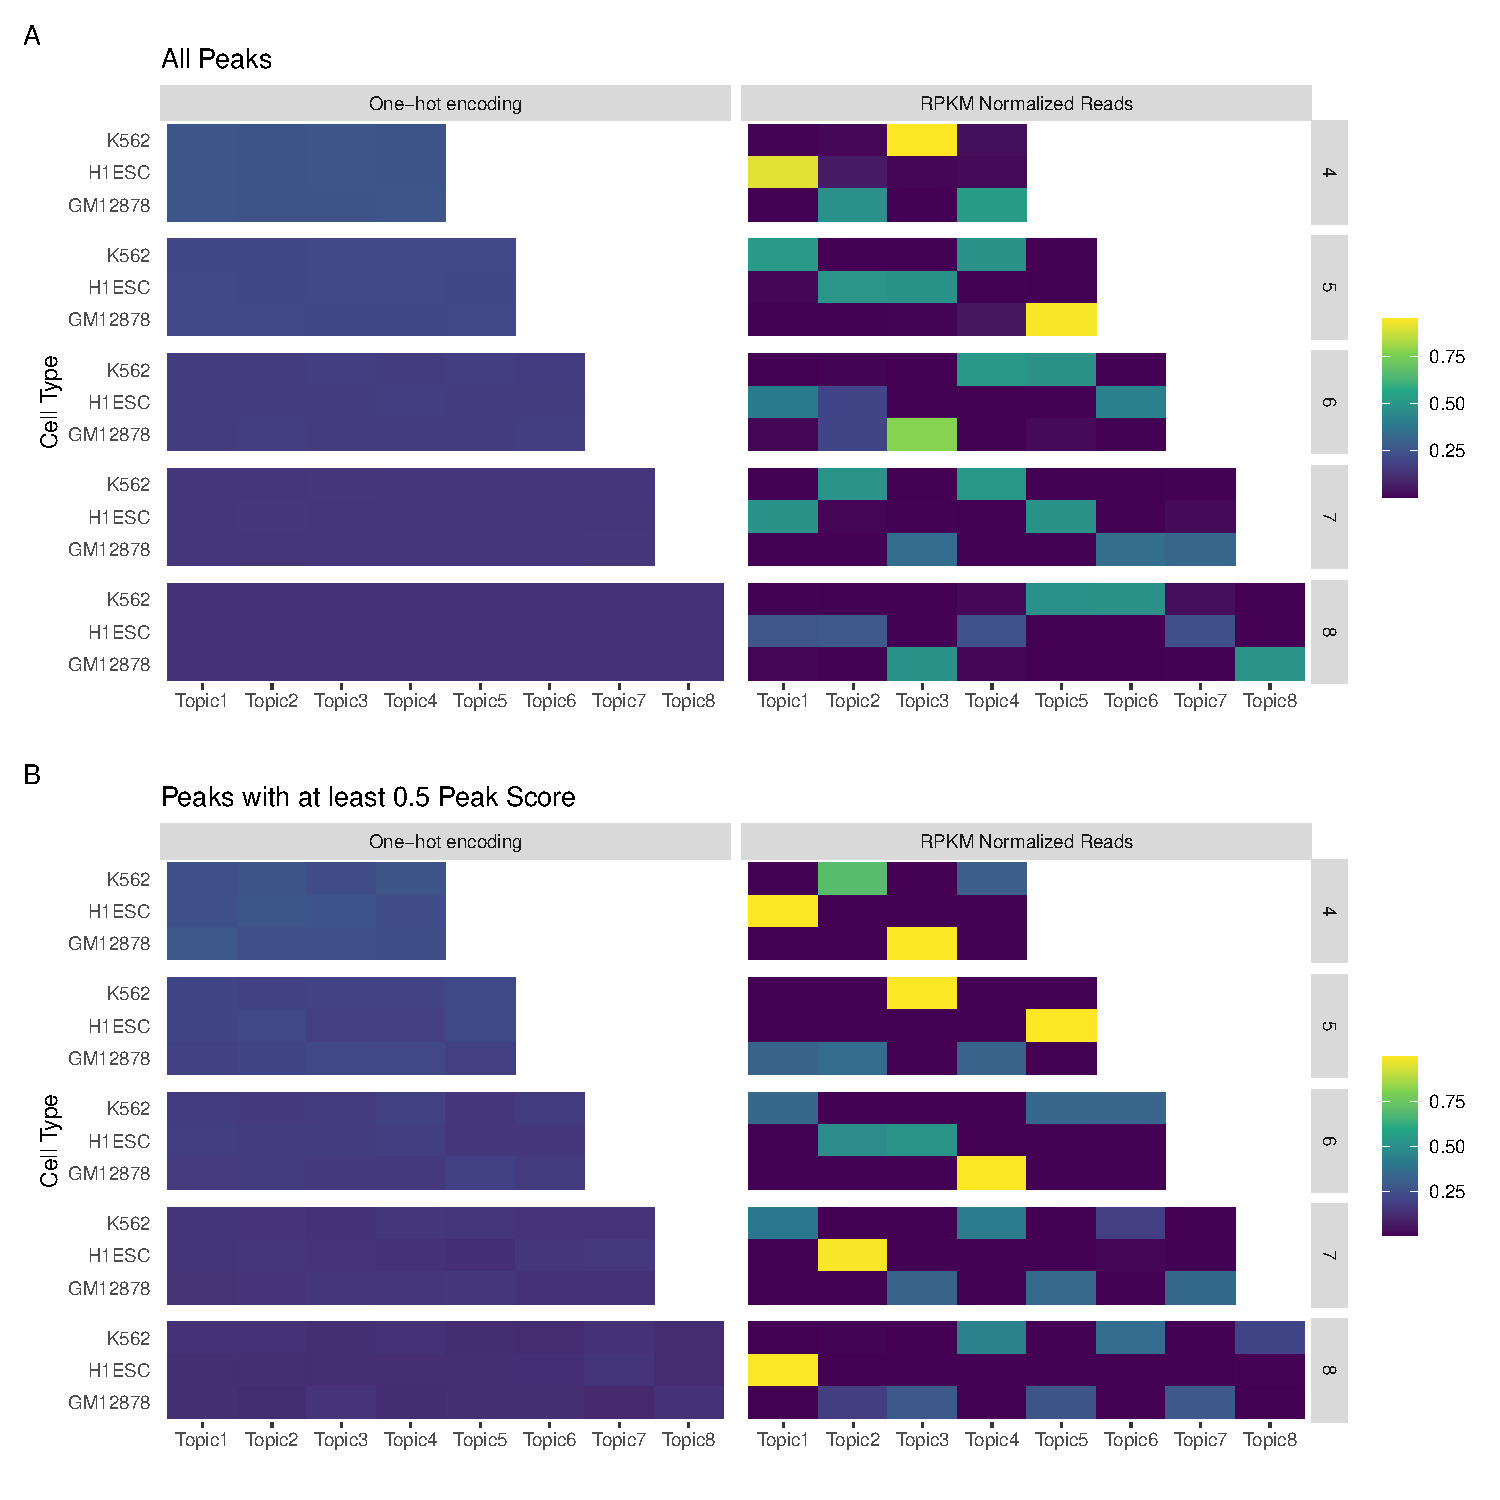
\includegraphics[width = \textwidth]{plot/ch4/pb_thresholding_topics.pdf}
  \caption{Inferred topic loadings using optimized hyper-parameters and \textit{a priori} defined for both the OHE and BLDA methods using pseudo-bulked scATAC-seq data.}
  \label{fig:pb_no_thresh_lot_topics}
\end{figure}

To investigate to what degree the BLDA procedure found regions which were differentially accessible across pseudo cell-types, we compare the "key word" regions to the regions selected by edgeR in \Cref{ch4:edgeR}. We use cisTopic's built in procedure for selecting important contributory regions to topic definitions, fitting a gamma distribution to the shape of the region-topic distribution for each topic and selecting regions which lie in the top 1\% of that distribution. Doing this, we find a difference in the number of regions identified between the thresholded and non-thresholded LanceOTron peak calls, which we expect given the selection procedure (\Cref{fig:pb_tot_number}). More peaks are also uniformly selected for the BLDA method, though we expect that this is due to the lack convergence in the classic LDA set up, rather than a systematic difference based on the method. 

\begin{figure}
  \centering
  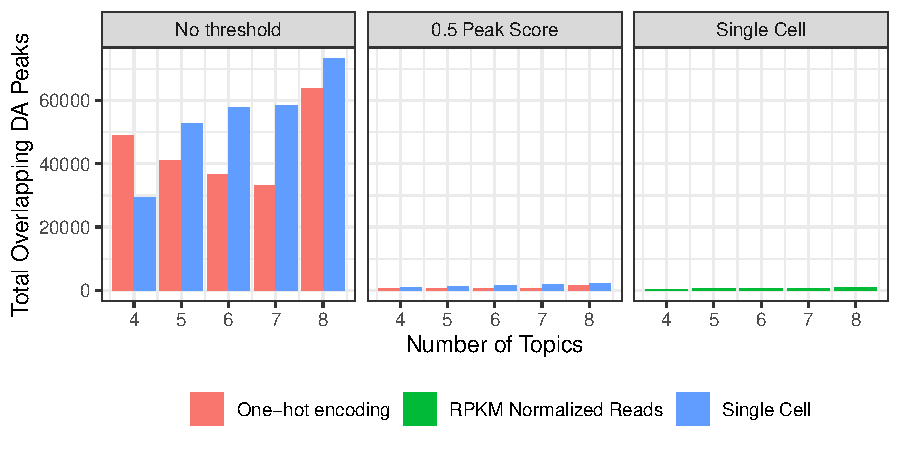
\includegraphics[]{plot/ch4/pb_diff_acc_tot.pdf}
  \caption{Total number of selected "key-word" regions for a given topic number between the two pseudo-bulk approaches, the two peak calling methods (thresholded and non-thresholded LanceOTron) and single cell analyses.}

  \todo{Colours are wrong here, fix this.}
  \label{fig:pb_tot_number}
\end{figure}

However, we find that the key-word regions are not equally specific with regards to the "ground-truth" differentially accessible regions from edgeR. Taking the top 100 regions from the edgeR analysis, we overlap them with all key-word regions in a given analysis (\Cref{fig:pb_olap_number}). 

Firstly, we find a clear difference between OHE and BLDA in their ability to identify truly differentially accessible regions (First versus second panel of \Cref{fig:pb_olap_number}). Considering the case of thresholded peak calls, OHE identifies almost none of the known differentially accessible peaks, while the BLDA method identifies slightly fewer than the original single cell experiment. This supports the assertion that bulk LDA is a comparable approach to single cell LDA for datasets consisting of a small number of dense cells. 

\begin{figure}
  \centering
  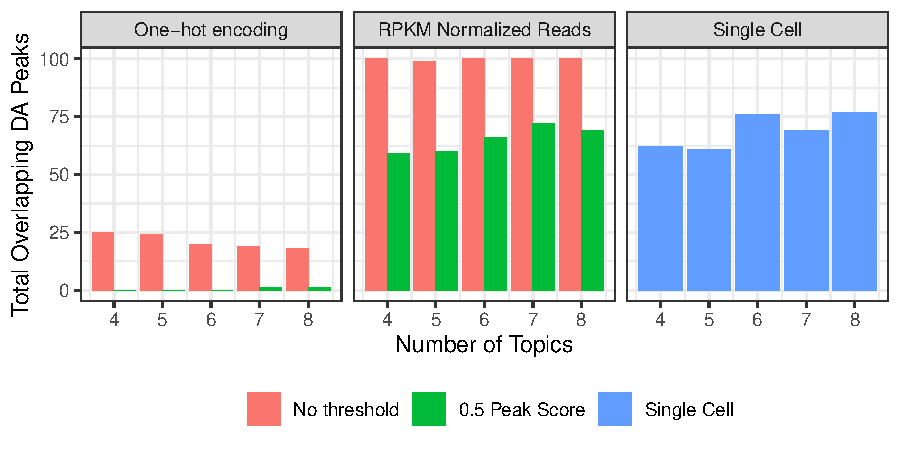
\includegraphics[]{plot/ch4/pb_diff_acc_olap.pdf}
  \caption{Number of overlapping regions between the top 100 differentially accessible regions determined by EdgeR and key-word regions selected by taking the top 1\% of a fitted gamma distribution for several LDA analyses. }
  \label{fig:pb_olap_number}
\end{figure}

\subsection{Bulk LDA describes Erythropoiesis}

Having established that BLDA is able to identify realistic patterns in bulk data, we investigate a well-characterized biological system. Erythropoiesis, the process by which red blood cells are produced, involves known differentiation stages with defined marker genes. This allows us to compare the topics inferred from BLDA with expectations based on the biology of the system.

\todo{Damien did this, how can I make this clear? I also dont exactly know how he did the aligning and stuff}

To create a dataset of bulk ATAC-seq data to study erythropoiesis, we download and process raw sequencing data from \textcite{Ludwig2019} and \textcite{Corces2016} using gene expression omnibus datasets GSE115684 and GSE74912 respectively. . Raw reads were assessed for quality with FastQC and aligned using. Coverage tracks were created using DeepTools and peak calling was performed using LanceOTron using the same score cutoff as previously described. The number of peaks identified this way varied considerably across cell types (\Cref{fig:ludwig_shared_peaks}A). Accessible regions of the genome generally increase from hematopoetic stem cells (HSCs) to common myeloid progenitors before decreasing in Megakaryocyte–erythroid progenitor cell. Erythrocyte colony forming units (CFUE) and orthochromatic erythroblasts (OrthoE cells) have especially accessible chromatin, with nearly 50,000 accessible regions. As it is known that nuclear chromatin condenses in preparation for enucleation in terminally differented immature erythroblasts, accesibility and the number of identified peak regions are greatly decreased in erythroblasts here as well \cite{Schulz2019}. There is relatively low sharing of accessible regions outside of a central differentiation "block" between ProE and BasoE cells (\Cref{fig:ludwig_shared_peaks}B). This too is consistent with our expectation, as terminal differentiation is known to significantly alter the expression of many hundreds of genes \cite{Schulz2019}. It is now well understood to what degree the differential usage versus differential accessibility of key regulatory elements shapes normal differentiation of human cells \cite{Song2011,West2014}. Here we use the previously characterized bulk LDA to identify groupings of accessible regions which are associated with specific stages in erythropoiesis. 


\begin{figure}
  \centering
  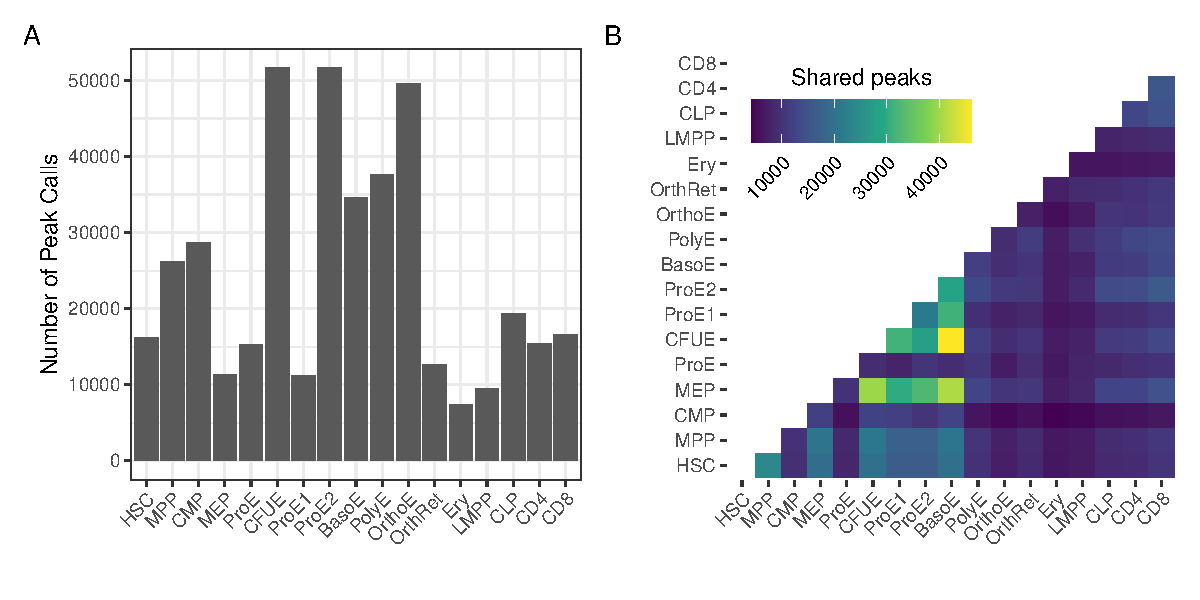
\includegraphics[width=\textwidth]{plot/ch4/ludwig_shared_peaks.pdf}
  \caption{Peak calling in erythropoiesis dataset. A. Number of identified peak regions by cell type using LanceOTron and a score threshold of 0.5. B. The number of peaks shared between cell types.}
  \label{fig:ludwig_shared_peaks}
\end{figure}

Peak calls were merged to create two count matrices. The first represents the typical cisTopic analysis method, one-hot encoding each peak region from its derivative cell type. The second is our BLDA method, using an integer value of RPKM normalised read count for each identified accessible region. We optimise the hyper-parameters as before, and run inference for between 8 and 20 topics. The number of topics was chosen to demonstrate, on the lower end, how LDA will group similar cells when it is forced to, and on the upper end if there is any remaining structure after each cell is allowed its own topic. We find that, similar to pseudo-bulked scATAC-seq data, the BLDA method consistently produces cleaner and better defined topic loadings for individual cell types (\Cref{fig:ludwig_quick_topics}). While this larger and more realistic dataset allows the OHE strategy to pick out some topics which differentiate between cell types, the patterns tend to be strongly constrained to certain grouping such as the erythroid precursors or lineage committed cells. The BLDA method on the other hand distinguishes highly cell-specific topics. The number of topics which are shared across multiple cell types varies considerably as the model is given more freedom with increasing number of topics. Even at low numbers, highly differentiated cell types like CD4 and CD8 T cells show distinct, highly enriched topics. Conversely, topics are almost always identified which are enriched in closely related intermediary cell types. We quantify the number of times two cell types share an enriched topic, taking a cell-normalised topic loading threshold of 0.25 to indicate enrichment (\Cref{fig:ludwig_quick_coenriched}). Two blocks of co-enriched cell types are obvious, one beginning from erythroid progenitors (ProE) and ending with basophilic erythroblasts (BasoE), the second beginning with BasoE and ending with Erythroblasts (Ery). It is rare for a cell type in either one of these clusters to share topic loadings with the other. Additionally, topics are occasionally shared between sequential stages of early differentiation, i.e. between hematopoetic stem cells and multi-potent progenitors (MPPs), but these topics never overlap with lineage committed cell stages.  

\todo{Add in the selected hyper-parameters table. }

\begin{figure}
  \centering
  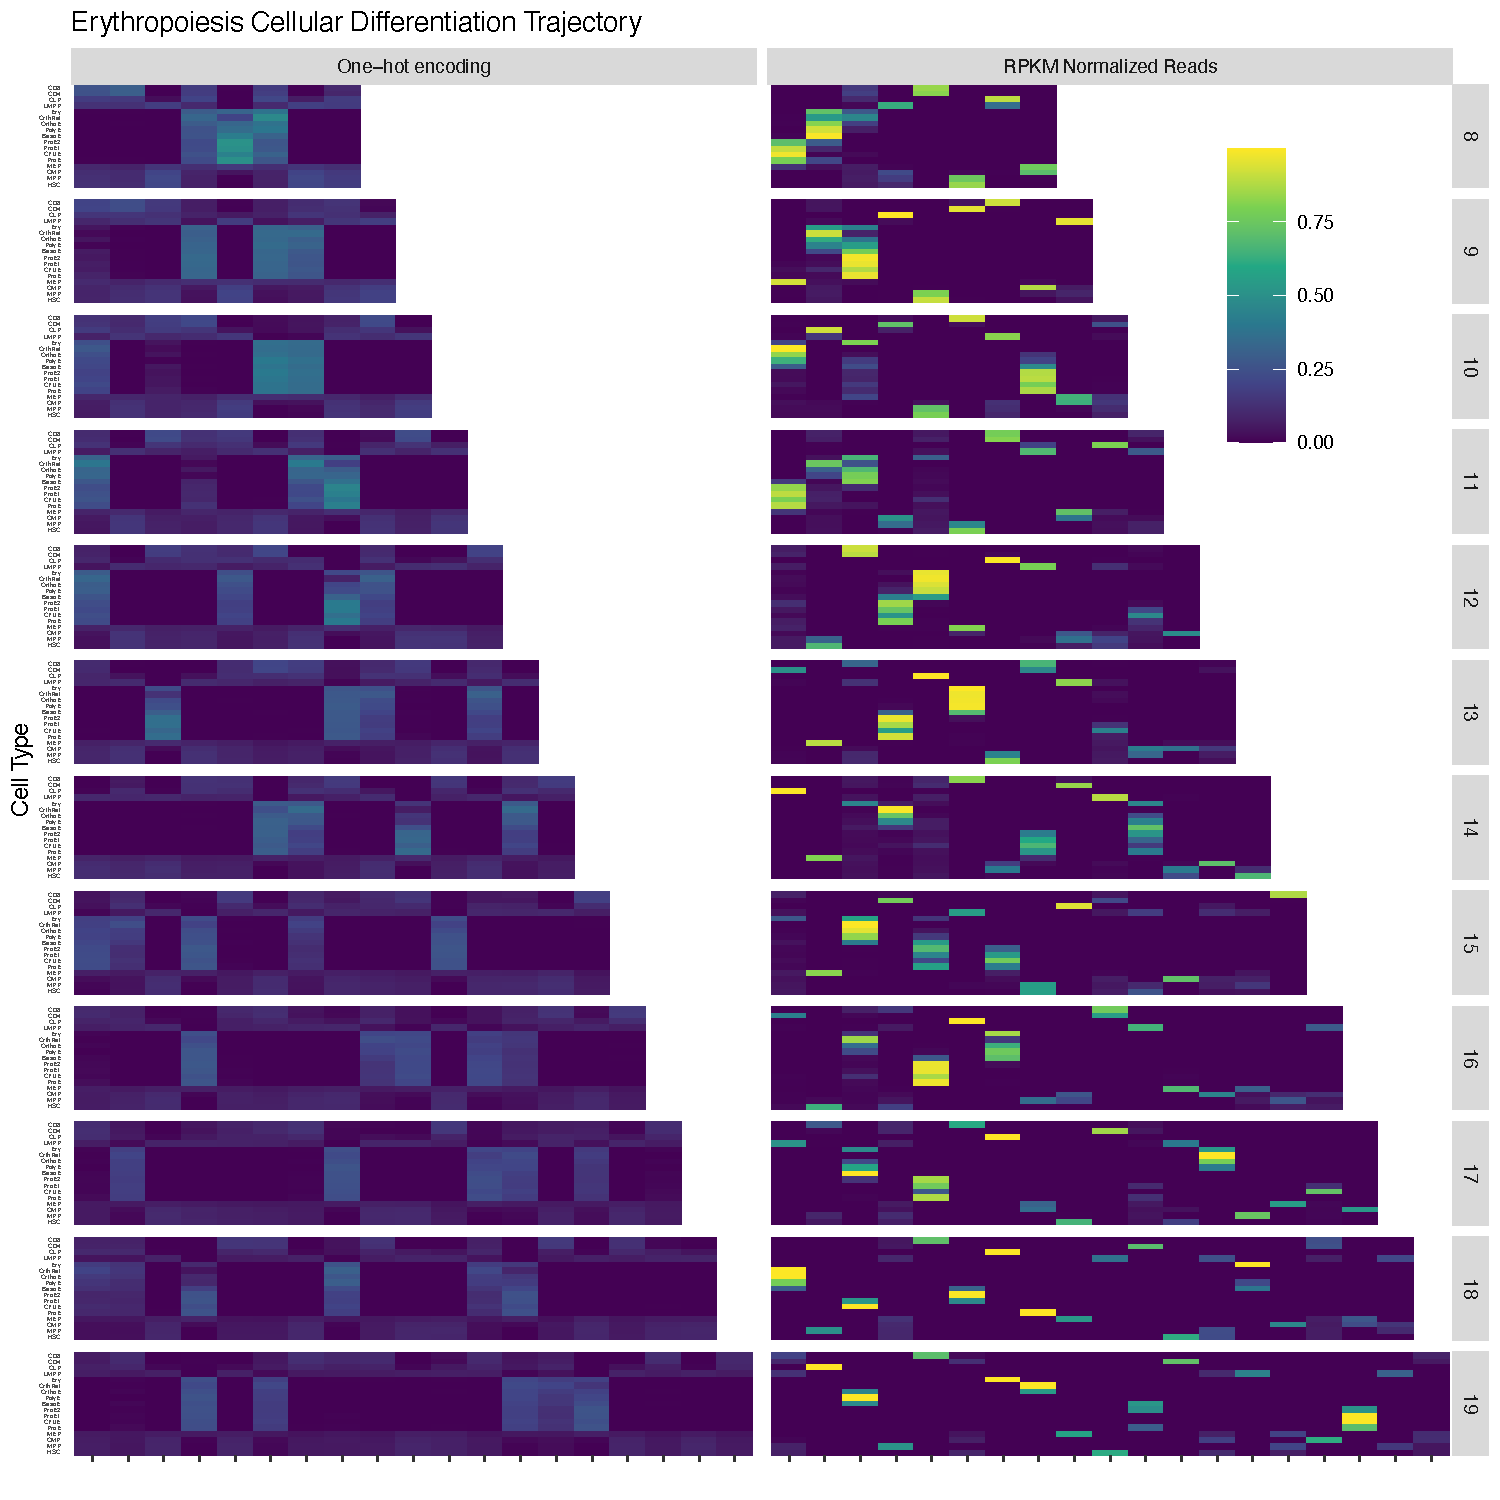
\includegraphics[width=\textwidth]{plot/ch4/ludwig_quick_topics.pdf}
  \caption{Inferred topic loadings for erythropoiesis dataset. On the left hand side, One-hot encoded LDA, on the right bulk LDA with RPKM normalization. Facets indicate the number of modelled topics. }
  \label{fig:ludwig_quick_topics}
\end{figure}

\begin{figure}
  \centering
  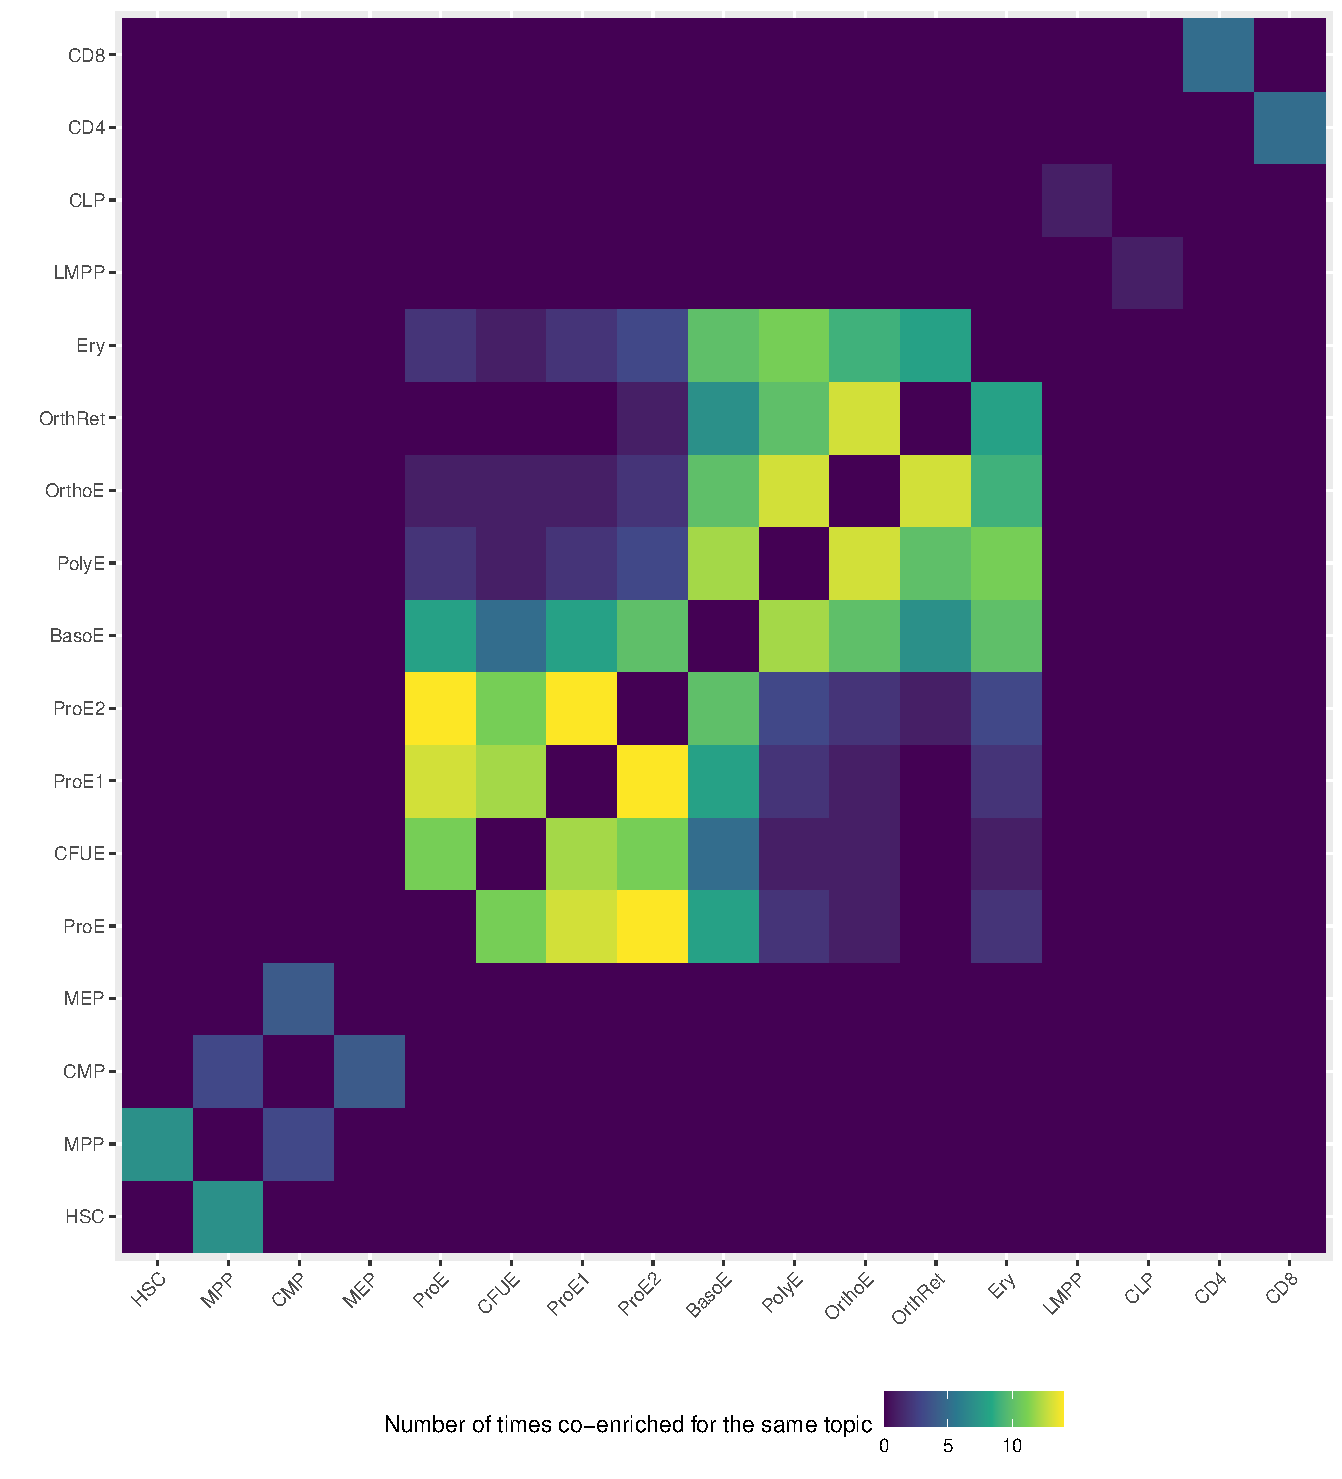
\includegraphics[width=0.5\textwidth]{plot/ch4/ludwig_coenriched.pdf}
  \caption{Similarity of cell types based on the number of times they are co-enriched for a topic, summarized over all numbers of inferred topics. Topics inferred using BLDA for the erythropoiesis dataset.}
  \label{fig:ludwig_quick_coenriched}
\end{figure}

\subsubsection{Isolating key-word regions from region-topic loadings}

Certain regions are inferred to be uniquely important for a topic. We follow the convention within the LDA literature in calling these samples key-words, as the observations within a document are typically denoted as words. There is no theoretical definition of a key-word region, therefore a threshold on the region-topic distribution must be empirically chosen to represent the most important regions. The cisTopic method normalizes the distribution of loadings within a topic such that it falls in the range 0-1 and theoretically follows a Gamma distribution, though the parameters for this distribution must again be inferred empirically. In this section, we attempt to identify sensible thresholds for key-word regions based on topic loadings. 

To decrease the number of variables that need to be studied, for this section we will focus on the BLDA inference. Based on the qualitative results from the previous section, quantitative input to the LDA inference algorithm produces more specific topics which are shared amongst related cell types in realistic ways. This specificity is important for the identifications of key-word regions. 

Additionally, we begin our analysis by focusing on only one value for the number of topics. For the analysis with $k = 16$ topics, SciPy was used to estimate the parameters of a Gamma distribution for the region-topic distribution for each of the 16 topics. Four thresholds were used to select the top 2.5, 1, 0.1, and 0.01\% of the inferred Gamma distribution. The number of selected regions ranged considerably across the topics (\Cref{fig:ludwig_topics_gamma}). From this we conclude that a gamma distribution may not fit each of the topics equally well, as the proportion of peaks that were selected based on the threshold does not reflect the theoretical expectation. 

To investigate further, descriptive statistics are used to identify candidate distributions. We use a Cullen a Frey graph to examine one of the poorly fit topics from \Cref{fig:ludwig_topics_gamma}, topic 8 (\Cref{fig:ludwig_topic8_distr}). 1000 bootstraps of the data indicate two potential distributions, gamma and lognormal (top left of \Cref{fig:ludwig_topics_gamma}). Maximum likelihood is used to estimate parameters for these distributions, and the empirical versus theoretical density, percentiles, and cumulative distribution functions are plotted (top right, bottom left, and bottom right of \Cref{fig:ludwig_topics_gamma} respectively).  Though it appears as though the density at least visually matches the gamma distribution, the larger empirical percentiles of the data do not match either a gamma or log-normal distribution (bottom left of \Cref{fig:ludwig_topic8_distr}). It seems likely that the skew of the data is causing the under-representation of selected key-word regions. 


\begin{figure}
  \centering
  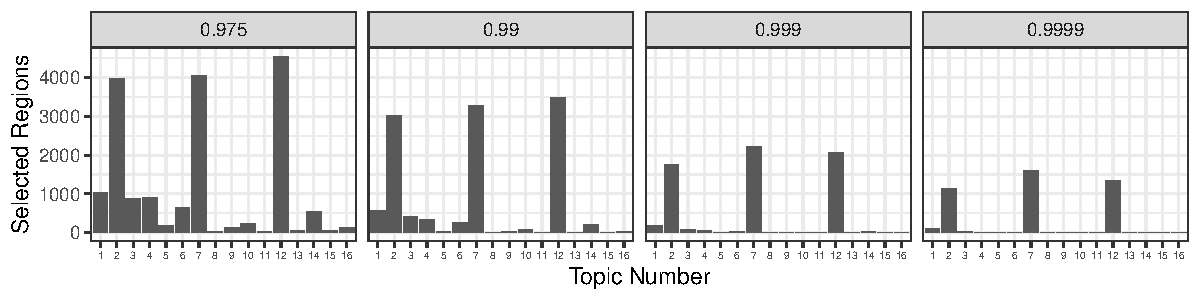
\includegraphics[width=\textwidth]{plot/ch4/ludwig_topics_gamma_16.pdf}
  \caption{Number of identified regions above the facetted percent point function of a Gamma distribution with inferred parameters using SciPy.}
  \label{fig:ludwig_topics_gamma}
\end{figure}

\begin{figure}
  \centering
  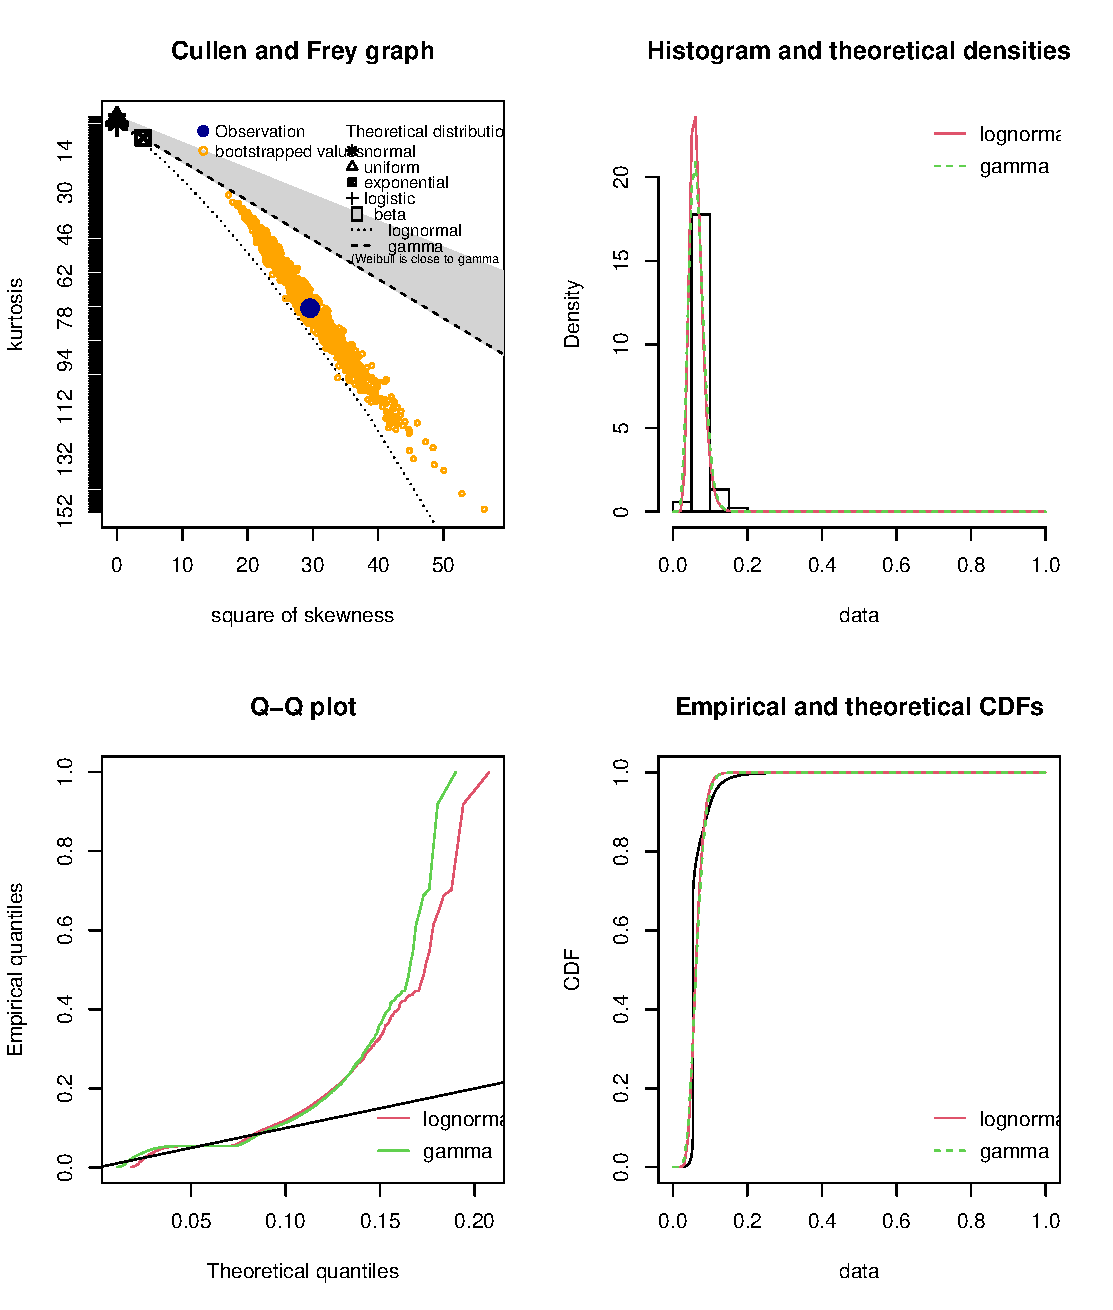
\includegraphics[width=\textwidth]{plot/ch4/topic8_distribution.pdf}
  \caption{Distribution of the region-topic distribution from a candidate topic from \Cref{fig:ludwig_topics_gamma}, topic 8. Top left shows a comparison of 1000 bootstrapped values of the data against descriptive statistics for several common distributions. Top right shows the empirical histogram of the data compared against the two distributions nominated from the Cullen and Frey graph fitted via maximum likelihood estimation. Top left shows empirical versus theoretical percentiles from the two fitted distributions, while bottom right shows the empirical cumulative distribution function.}
  \label{fig:ludwig_topic8_distr}
\end{figure}

This lack of fit to a theoretical gamma distribution presents several avenues for exploration. One option would be to fit a mixture distribution, explaining different portions of the data with different parameters for the distributions. However, this would make it difficult to estimate a certain proportion of the overall distribution, which is the goal of the exercise. Instead, we opt to take the simpler route and simply take a fixed number of the highest region-normalised topic loadings. This guarantees a sufficient sample size for further analyses like motif identification and pathway enrichment, while not making the analysis overly complex for replication across the different $k$ values of topics.

\subsubsection{Motif enrichment within key-word regions}

The top 100, 250, and 500 regions from each region-topic distribution are selected and MotifScan (\url{https://motifscan.readthedocs.io/en/latest/}) is used along with the JASPAR database of \gls{tfbs} motifs to identify regions matching known \gls{pwm} and find over-representation in the set of regions. A control set of regions is constructed by taking the negative intersection between the original merged dataset of regions and the selected regions, in order to better represent both accessible DNA and relevant common motifs for the system. A second control set is constructed by taking the union of all regions selected as key-word regions. This second set investigates motifs which are enriched relative to other selected regions.

The smallest $k$ topics forces sharing between similar cell types (\Cref{fig:ludwig_8_topic}). For each topic, the enrichment of all \gls{pwm} in the JASPAR database is calculated for each count of top regions, and each control strategy (\Cref{fig:ludwig_motifs_8}). Some topics in this particular instance are of interest. Topic 6 spans the early developmental stages between hematopoetic stem cells and multi-potent progenitors, and shows enrichment for known factors like MEIS1, whose expression is required for erythropoesis in HSCs \cite{Miller2016,Zeddies2014,Unnisa2012}.  

\begin{figure}
  \centering
  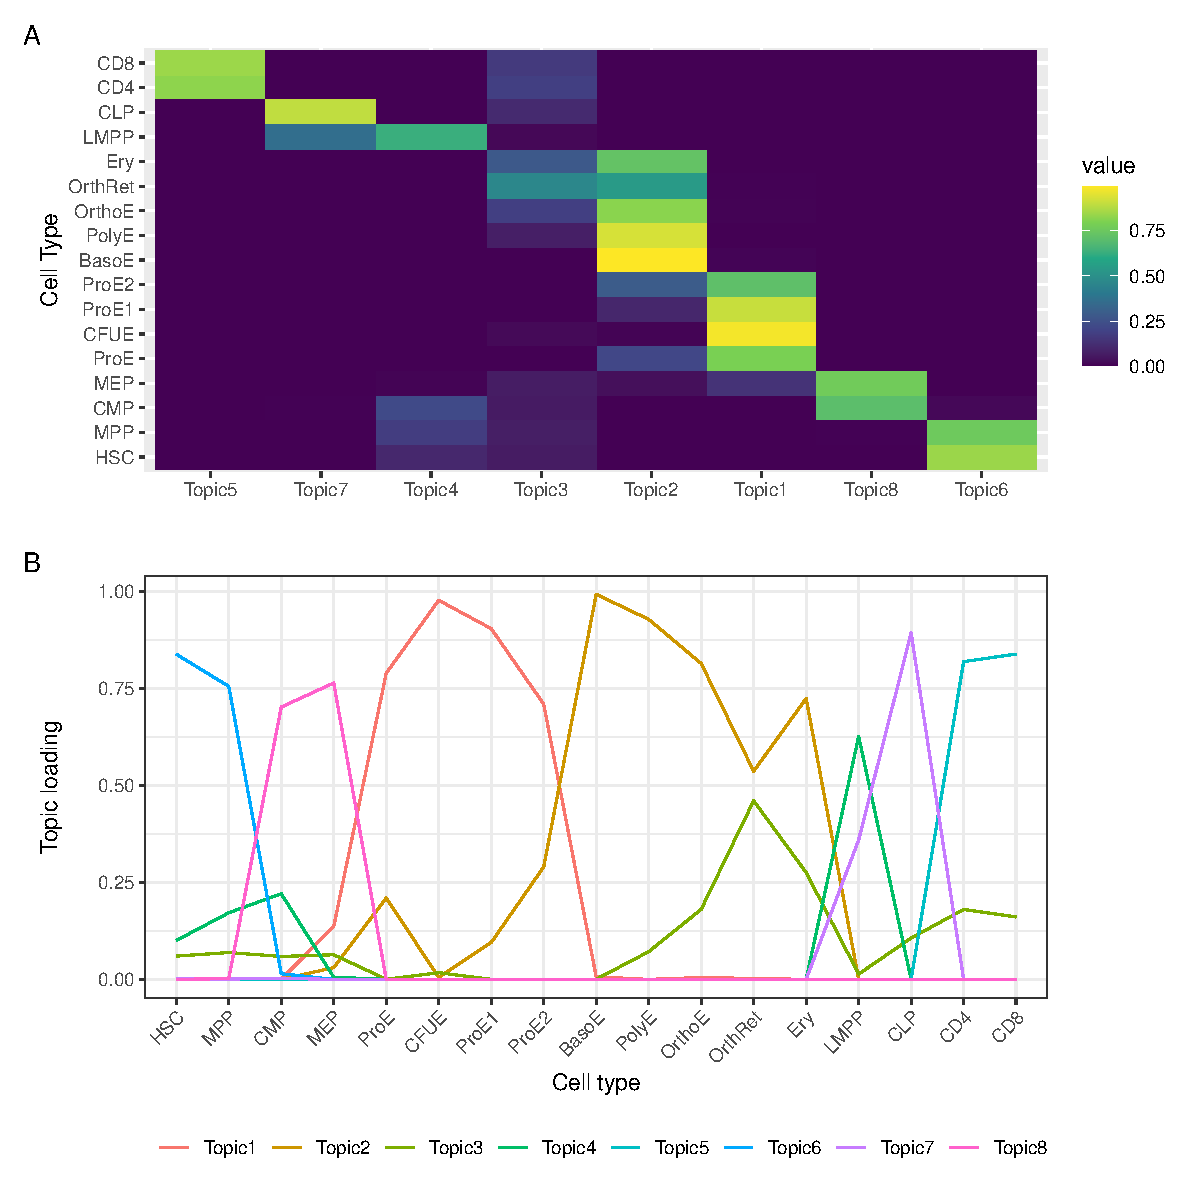
\includegraphics[width=\textwidth]{plot/ch4/ludwig_quick_topic_8.pdf}
  \caption{Cell-topic distribution for $k=8$ topic. A. Loadings across cell types ordered by differentiation trajectory. B. Loadings by topic across differentiation pseudo-time.}
  \label{fig:ludwig_8_topic}
\end{figure}

\begin{figure}
  \centering
  \includegraphics[width=\textwidth]{plot/ch4/ludwig_motifs_8.png}
  \caption{All identified motifs for $k=8$ topic analysis. The top 100, 250, and 500 topics were selected and enrichment was calculated either against all peak regions, or against all selected key-word regions. }
  \label{fig:ludwig_motifs_8}
\end{figure}

\subsubsection{BLDA identifies relevant pathways active in Erythropoiesis}

A combination of the motifs identified as well as the groupings of regions allows for a deeper interrogation of the uncovered biology.

\textcite{Ludwig2019} identified several regions of the genome with substantial impacts on the process of Erythropoiesis. Of these, there are no overlaps between UROS, CCND3, VEGFA, and TMCC2 in the set of selected keyword regions. However, the promoter region for the Rh associated glycoprotein (RhAG), which is not accessible in HSC, MPP, or CMP cells, shows a progressive increase in accessibility throughout erythropoesis, as shown in \Cref{fig:RhAG}. A keyword region for topic 2 is located in its promoter. Topic 2 mirrors the accessibility patterns of RhAG, showing  which also is shown to be inactive in early hematopoesis and increasing in accessible after lineage commitment, peaking in BasoE cells. Other examples of individual regions which mirror topic loading patterns are readily apparent, such as the R3HDM4 locus, which is also a key region for topic 2 (\Cref{fig:r3hdm4}). 

To comprehensively survey the closest annotated protein coding genes, bedtools was used to find the nearest genic regions to each of the key regions for the different topics. \textcite{Mello2019} recently surveyed differentially accessible genes throughout different phases of erythoiesis. These genes are compared against the nearest genic regions for the top 500 keyword regions from each of the topics. The results illustrate a close match between topic activation patterns and the underlying biology of blood cell differentiation.

Topic 1, active in early lineage commitment, include critical proteins for erythropoiesis such as STAT5A and STK3. STAT5a is predominantly expressed in early erythropoesis \cite{Pishesha2014}. The regions are enriched for the binding motifs of GATA2, GATA3, KLF1, and KLF12. GATA3 is typically associated with lymphoid precursors and committed T cells, recent results indicate a more ubiquotous role within hematopoesis \cite{Chen2001}. The topic shows no overlap with genes involved in apoptosis, unlike later topics.  

Topic 2 represents the main inferred mid-to-late erythropoesis grouping of regulatory elements. It contains the majority of important proteins involved in iron homeostasis and mitochondrial transportation (SLC25A38), heme production (ALAS2), regulation of cellular differentiation (SP1). In addition, SP1 represents the first protein involved with enucleation. An gene set enrichment analysis showed subenrichment for "Positive regulation of erythrocyte differentiation", indicating that a significant portion of the genes identified relate to erythropoiesis. Additional terms identified include "tetrapyrrole biosynthetic process", "tetrapyrrole metabolic process", and "pigment metabolic process". \todo{Table for the GO enrichment with panther} 

Topic 3 peaks in activity amungst orthochromatic erythroblasts, and also has some representation in early hematopoesis, as well as committed T cells. Topic 3 includes NRF1, a knockout of which leads to embryonic lethality due to impaired fetal liver erythropoiesis \cite{Chen2001}. GLRX5, predominantly expressed in late erythropoesis by poly and orthochromatic erythroblasts (Fig 1c \cite{Pishesha2014}) is also amungst the nearest key genes, along with FOXO3 and PPP2R1A \cite{Mello2019}. Topic 3 also shows enrichment for a large number of motifs, indiciative that a number of identified peak regions are not directly involved in protein coding but are intergenic enhancer elements (\Cref{fig:ludwig_motifs_8}).

Early hematopoesis is represented by topics 6 and 8, which are only associted with a handful of genes associated with erythropoesis (\Cref{table:mello_genes}). HIP1 is known to be crucial to successful hematopoesis and LYN is involved in the successful proliferation of hematopoetic cells \cite{Oravecz-Wilson2004, OLaughlin-Bunner2001}. Motifs in these regions include ARID3a, known to be expressed in HSCs, and MEIS1, also involved in early hematopoesis \cite{Zeddies2014,Miller2016, Ratliff2020}. 

These results indicate that BLDA has identified regions which correspond to realistic regions of differential accessibility throughout the process of erythropoesis. Though the method is not specific, in that many important regions are not represented amungst the results.  



%Later stages of erythopoesis, characted by ..., are also represented within the dataset. FOXO3, PPP2R1A known to be upregulated towards the end of the process, was identified within topic 3.  Topic 2 contained later genes such as TXNRD2, 




%Regions crucial for erythroid differentiation and survival are represented across the key regions for relevant topics. For example, topic 1 contains the promotor of STAT5a, topic 2 covered the ALAS2 gene, PARK7 is found in topic 3

%Different regions of FOXO3, a gene involved in immune response, were found associated with topics 3, 7, and 1. 

%Topic 2 


\begin{figure}
  \begin{subfigure}[b]{0.5\linewidth}
      \centering
      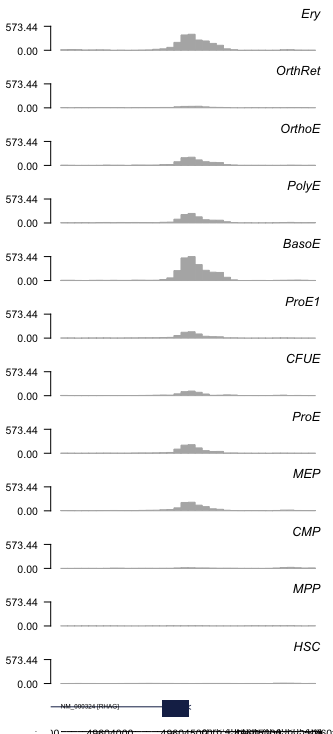
\includegraphics[width=\textwidth]{plot/ch4/RHAG}
      \caption{The RhAG promoter}
      \label{fig:RhAG}
  \end{subfigure}
  \hfill
  \begin{subfigure}[b]{0.5\linewidth}
    \centering
    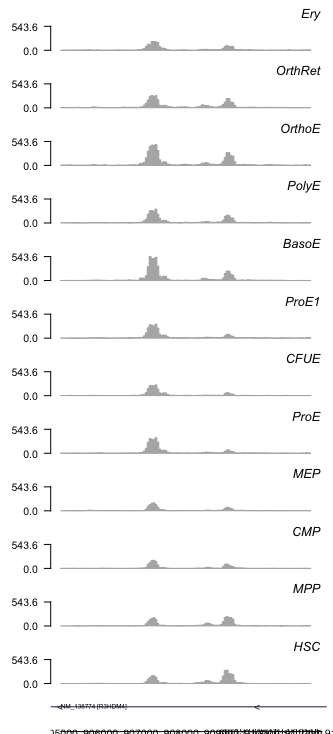
\includegraphics[width=\textwidth]{plot/ch4/R3HDM4}
    \caption{R3HDM4}
    \label{fig:r3hdm4}
  \end{subfigure}

  \caption{Accesibility at two keyword regions for topic 2 among cells in the erythropoetic differentiation trajectory. }
    
\end{figure}

\clearpage% Flush earlier floats (otherwise order might not be correct)
%\thispagestyle{empty}% empty page style (?)
\begin{landscape}

  \begin{table}
  %\resizebox{\textwidth}{!}{
    \tiny
\begin{tabularx}{\hsize}{|X|X|X|X|X|X|X|X|X|}
  
  \toprule
Category & Topic  1 & Topic  2 & Topic  3 & Topic  4 & Topic  5 & Topic  6 & Topic  7 & Topic  8\\
\midrule
Anti-apoptosis & CTSB & MKL1, BCL2L1, CTSB, NR3C1 & CITED2, PGAP2, TNFAIP3 & PDPK1 & HSPA9, NFKB1 & NA & NA & NA\\
Cellular component involved in apoptosis & ACTN4, KPNB1 & CDH1, KPNB1, GSN & PSMB1, RB1CC1 & ACTN4 & VIM & PSMB1 & DBNL & NA\\
Erythroblast enucleation & NA & SP1 & NA & NA & NA & NA & NA & NA\\
Erythrocyte differentiation & STAT5A & ALAS2, SLC25A38, BPGM, ERCC2 & CITED2, BPGM & NA & HCLS1, NCKAP1L & LYN & BPGM, DYRK3 & NA\\
Hematopoiesis \& regulation of cell differentiation & GFI1B, ZBTB16, TXNRD2 & BCL11A, SP1, TXNRD2 & GLRX5, PPP2R1A & TTC7A & IKZF1 & ZBTB16, LYN & IKZF1, CDK6, TTC7A & ZBTB16\\
Heme metabolism & ALAD, BLVRB, TMEM14C & ALAD, ALAS2, BLVRB, FECH, HMBS, SLC25A38, SPTA1, UROD & ALAD & FECH & NA & NA & NA & NA\\
Induction of apoptosis & LGALS1, MAPK1, SPN, DAPK2, SAP30BP, VAV1 & KAT2B, RBM38, TP53BP2, AKAP13, ERCC2 & BCLAF1, PPP2R1A, STK17B, TP53BP2, BTG1, NMT1 & CUL3, KAT2B, HIP1 & RBM38, MAP3K5, APP & HIP1 & HIP1 & MAP3K5\\
Iron homeostasis & NA & UROD & FBXL5, SLC25A28 & NA & NA & NA & NA & NA\\
Oxygen homeostasis/ response to hypoxia or to oxidative stress & ACTN4, MLH1 & HMBS, STAT5B, ERCC2, NRF1, PTK2B & CAT, CITED2, MLH1, OXSR1, PARK7 & ACTN4, PTK2B & ECE1, NFKB1, NR4A2 & IPCEF1 & NA & CAT, IPCEF1\\
Primitive hematopoiesis & STK3 & NA & NA & NA & NA & NA & NA & NA\\
\bottomrule
  \end{tabularx}
  %}

  \caption{Genes from \textcite{Mello2019} represented in the closest genes set of 500 keyword regions for each of the eight BLDA topics grouped by function.}
  \label{table:mello_genes}
\end{table}
\end{landscape}
\clearpage% Flush page


%  \begin{figure}
%  \centering
%  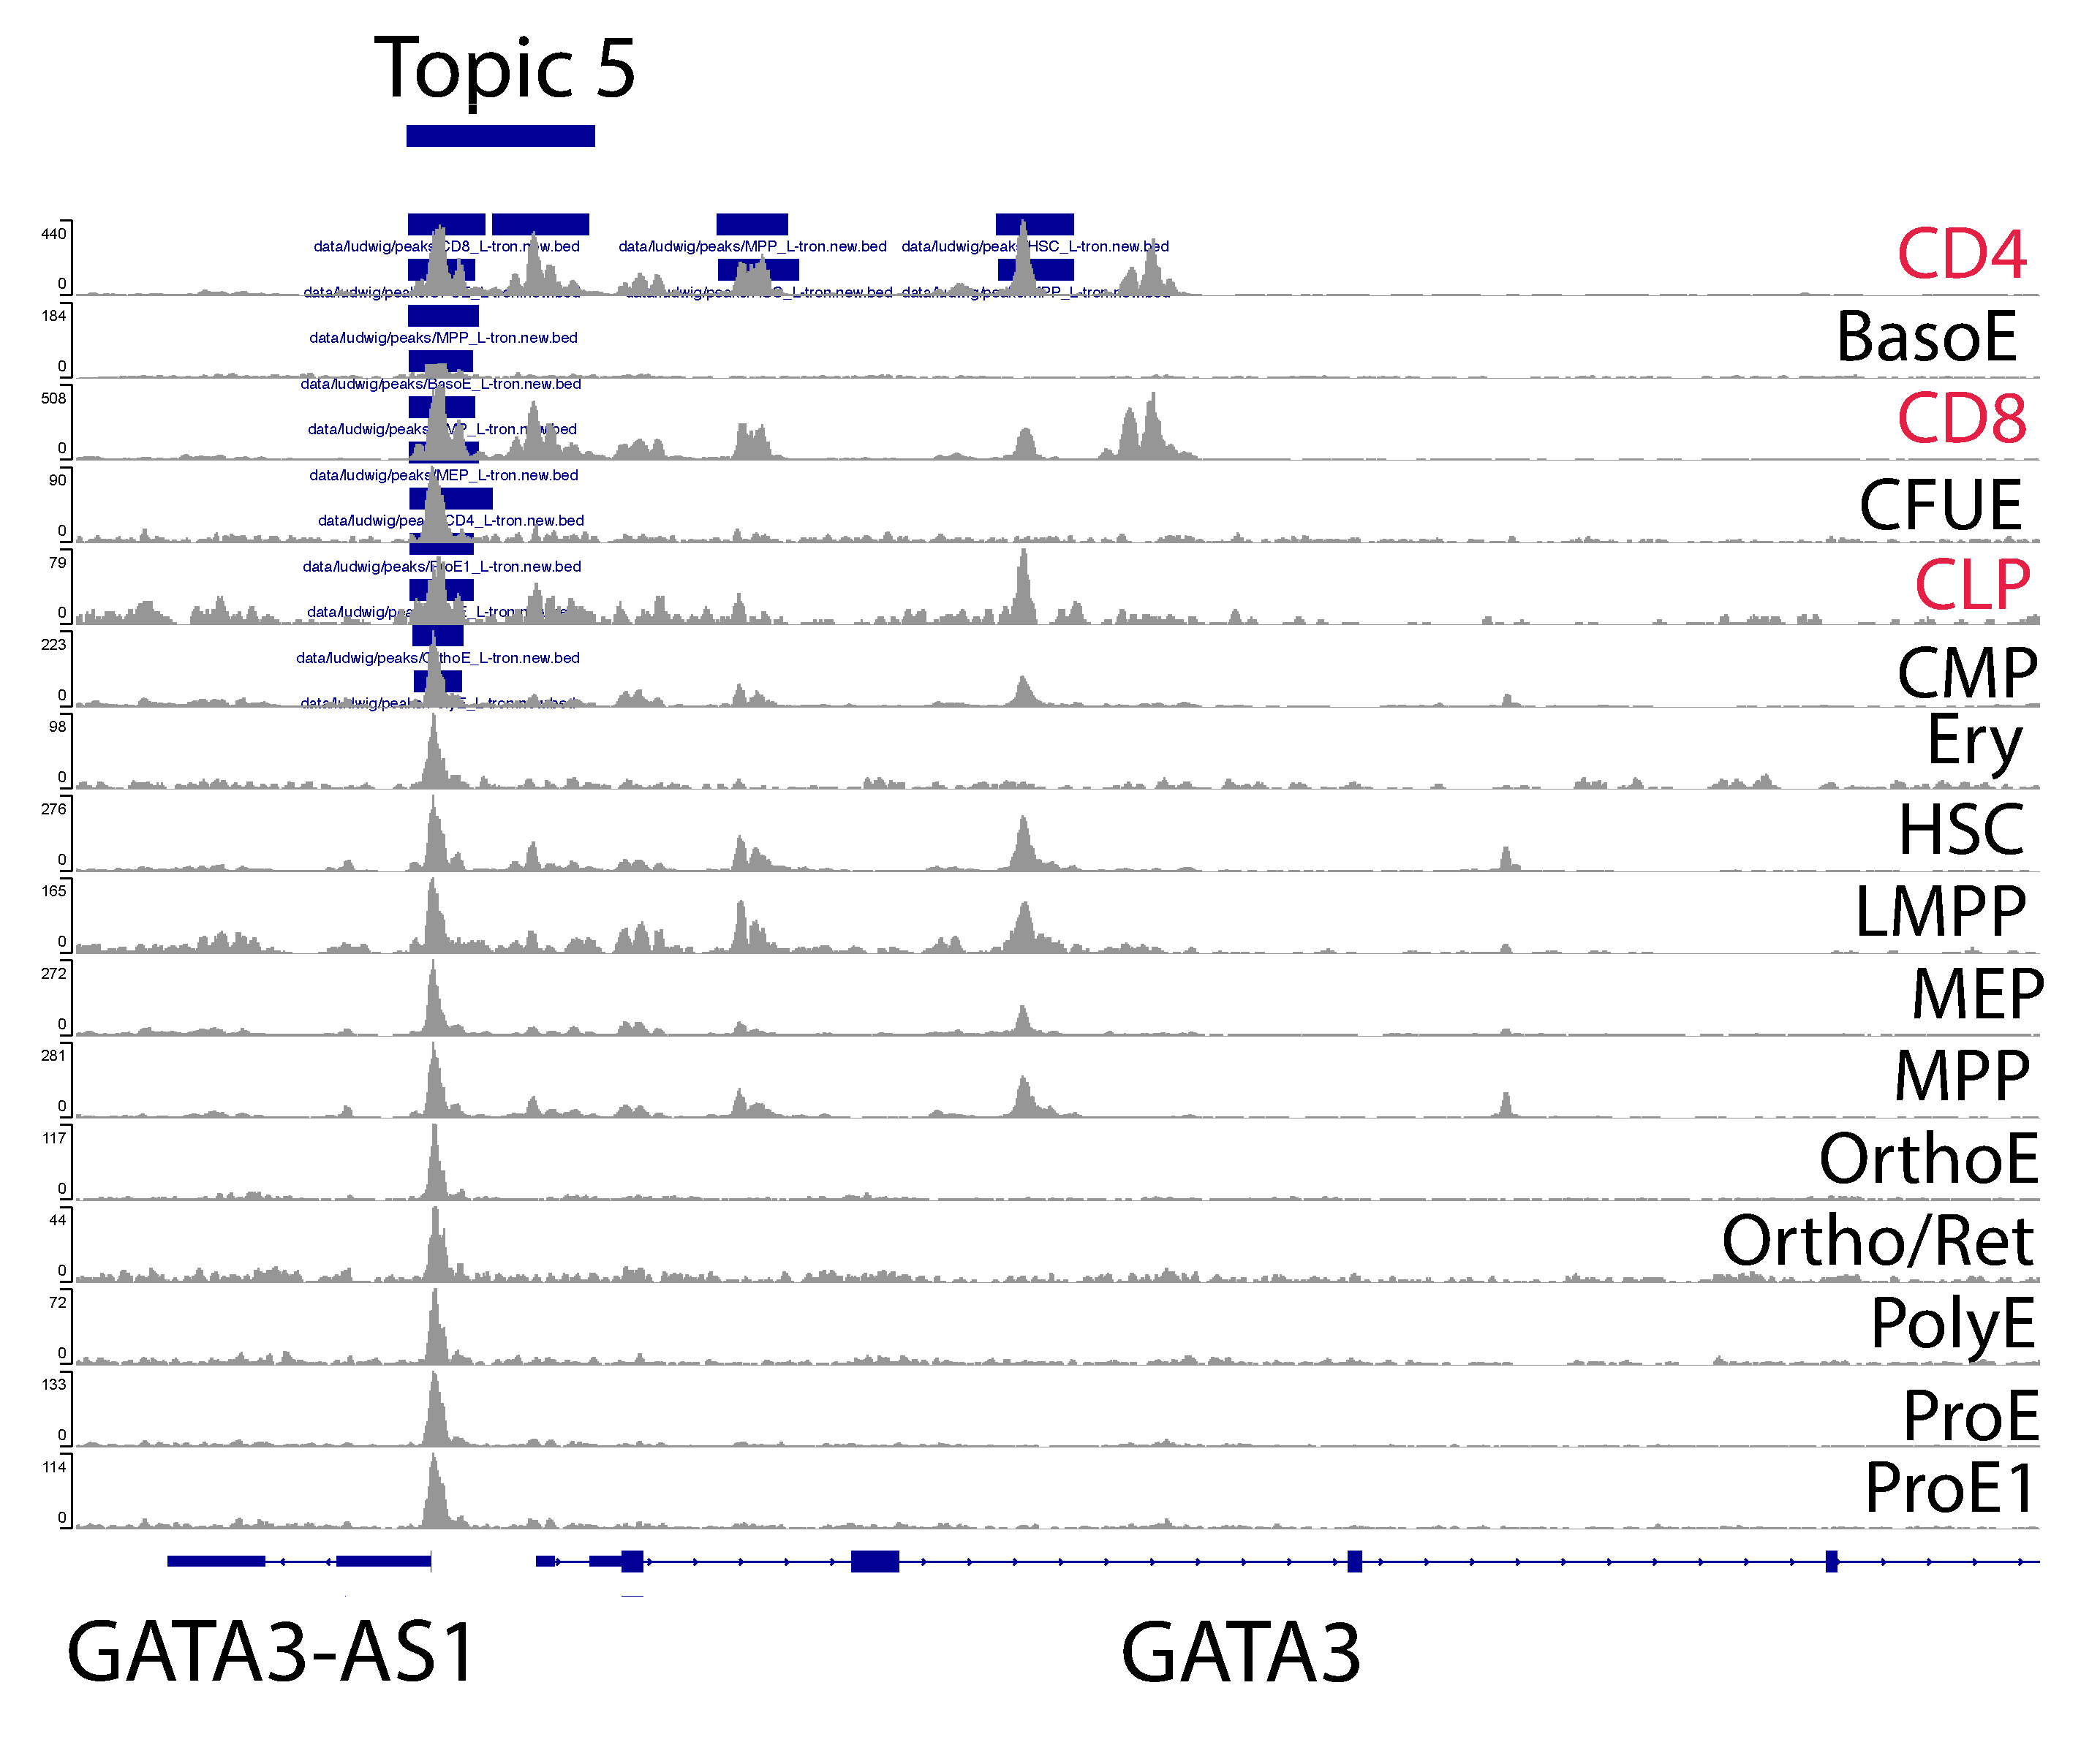
\includegraphics[width=\textwidth]{plot/ch4/GATA3.pdf}
%  \caption[GATA3 Promotor]{Coverage plot of the GATA3 promoter. BLDA identifies this region as discremintory for CD4 and CD8 T cells, and coverage plot indicates that it is differentially accessible between erythopoetic and terminally differentiated lymphocytes.}
%  \todo{Why is the other beds peaking through???}
%  \label{fig:gata3}
%\end{figure}


%Topic 1:
 % - Stat5a promotor is one of the most important regions. Stat5a is 
 %   -  regulation of RBC production by expansion of earlier progenitor and stem cell populations.
 %   - topic 1 esxpression starts early and ramps up through erythropoesis
 %   - (and 2) share a peak with MiR584. What role does this play?


%  Topic 8 (and 5)
%    - CGAS is widely expressed but especially in hematopoetic progeneitors (https://www.frontiersin.org/articles/10.3389/fimmu.2020.573915/full)

%Topic 2
%  - Many of the systems like UROS, CCND3, VEGFA, and TMCC2 are not found in this system.
%  - RHAG is found, peak accessibility in BasoE and the topic it is found in peaks with BaseO. 
%    - Expressed in mature 
%  - HDAC6, some role in enucleation,not completelysure (https://www.ncbi.nlm.nih.gov/pmc/articles/PMC5451330/)
%  - R3HDM4 is accessible in all of the cells, but differentially so. 
  %  - It's expession (RNA-seq) is associated with erythropoesis https://genevatool.org/gse_description?gene_name=R3HDM4&gse_id=GSE102182
  %  - Experssed in mature Erythrocytes https://genevatool.org/gse_description?gene_name=R3HDM4&gse_id=GSE63703



% Topic5:
 % - Has a promotor for GATA3. Maybe because this is not accessible in CD8 and CD4? But in everything else? 
   % - Motifs found in almsot every other cell type
 % - Actually also important for t cells https://www.ncbi.nlm.nih.gov/pmc/articles/PMC3688666/

%Early: 
%  - Arid3a / bright (6)
%  - MEIS1 is expressed prefernetially in HSCs (https://www.ncbi.nlm.nih.gov/pmc/articles/PMC3525022/)

\section{Discussion}

Recently, the use of \gls{atac} to characterise chromatin accessibility in varied cell systems has resulted in an excess of high quality data. However, it is currently difficult to integrate these data and perform inference for common regulatory programs. In this chapter, I adapted the cisTopic approach for using \gls{lda} to simultaneously infer weighted collections of co-accessible regions and the cell types in which they are active. I show that the method, BLDA, is able to identify a similar number of differentially expressed regions (as defined by EdgeR) as the established \gls{scatac} pipeline in a collection of pseudobulked single cell experiments with known cell types. The modification was essential to its comparative success, as a naive implementation of the cisTopic algorithm using region thresholding and one-hot encoding did not identify any of the same differentially accessible regions as the single cell analysis. BLDA additionally identified topics which were much more specific to target cell types than the naive implementation, as is expected in a purpose-built dataset of dissimilar cell types (\Cref{fig:pb_no_thresh_lot_topics}). This simple dataset shows that BLDA is able to recreate some of the success of the single cell method in bulk samples, so I next turn to a well understood system of differenting cell types. Erythropoiesis, the process by which \glspl{hsc} differentiate into red blood cells, or here more specifically immature erythroblasts which have not yet undergone enucleation, has an extensive literature documenting genes which are up and down regulated at various check points \cite{Ludwig2019}. We take sequencing data from \textcite{Ludwig2019} and \textcite{Corces2016} and create a pseudo-timed differentiation trajectory incorporating hematopoietic precursors and erythropoietic check points, as well as stages of the lymphoid differentiation pathway incorporating CD4 and CD8 positive T cells. I show that in this system as well, the BLDA method out performs a naive implementation of cisTopic, identifying specific topic loadings that are enriched for the regulatory biology of erythropoiesis. Infered topics identify regions of the genome which are shown to be differentially accessible in similar patterns to topic loadings across pseudo-time such as \Cref{fig:RhAG} and \Cref{fig:r3hdm4}. 

Having established that BLDA has power to find biologically enriched pathways within topic loadings, the next chapter applies the algorithm to large scale datasets of ATAC-seq experiments like ENCODE and uses them to investigate cell types with relatively unknown regulatory grammar.  

\section{Data and Code Availability}

Single cell sequencing experiments from \cite{Buenrostro2015} are available via SRA, and scripts for performing peak calling and pseudobulking are distributed with the BLDA package at \url{https://github.com/Chris1221/BLDA}. This package also contains functionality for creating count matrices from BAM files and bigWig tracks in order to run the adapted analysis pipeline. A modified version of cisTopic necessary for running these analyses is available at \url{https://github.com/Chris1221/cisTopic_bulk}. 

Data for the erythropoiesis developmental trajectory is available from GEO, with more details about specific file formats available from the original publications \textcite{Corces2016} and \textcite{Ludwig2019}.

An implementation of LanceOTron peak caller for batch data is available from \url{https://github.com/Chris1221/LanceOTron}.

A Snakemake pipline for replicating the entirety of the analyses presented in this chapter is available in the chapter\_3 subdirectory of \url{https://github.com/Chris1221/thesis_lda} repository.

\section{Acknowledgments}

The original conception of the BLDA extension, that is incorporating read counts rather than binary accessibility into the count matrix, came from Alastair Smith. Single cell experiments were downloaded and combined into a single BAM file by Emine Ravza Gur. Alignment and quality control of the datasets from \textcite{Corces2016} and \textcite{Ludwig2019} was performed by Damien Downes. 
%%\begin{savequote}[8cm]
%\textlatin{Neque porro quisquam est qui dolorem ipsum quia dolor sit amet, consectetur, adipisci velit...}

%There is no one who loves pain itself, who seeks after it and wants to have it, simply because it is pain...
%  \qauthor{--- Cicero's \textit{de Finibus Bonorum et Malorum}}
%\end{savequote}

\chapter{\label{ch:2-nn} Machine Learning, or something like that} 

\minitoc









%% APPENDICES %% 
% Starts lettered appendices, adds a heading in table of contents, and adds a
%    page that just says "Appendices" to signal the end of your main text.
\startappendices
% Add or remove any appendices you'd like here:
\chapter{Demographic Models} \label{app:dem_model}

Generally, these models can be implemented in either {\tt scrm} or {\tt ms} through they have been written with the former in mind.

\section{Seed model for SMCSMC Inference} \label{app:dem_model:seed}


We seed the particle filter with a demographic model of population size and uniform symmetric migration rate, given by the following {\tt scrm} command:

\begin{Verbatim}[fontsize=\tiny]
-ej 0.2324 2 1 -eM 0 1 -eN 0.0 6 -eN 0.0037 4.4 -eN 0.0046 3 -eN 0.0058 2 -eN 0.0073 1.4 
-eN 0.0092 0.85 -eN 0.093 1.2 -eN 0.12 1.7 -eN 0.15 2.2 -eN 0.19 2.5 -eN 0.24 2.4 
-eN 0.30 2.0 -eN 0.37 1.7 -eN 0.47 1.4 -eN 0.59 1.2 -eN 0.74 1.0 -eN 0.93 0.91 -eN 1.2 1.6
\end{Verbatim}

\section{Migration Simulations}

The following models were used for population sizes:

\subsection{African Population Size}

\begin{Verbatim}[fontsize=\tiny]
    -en 0.00000000 1 36.9124479 -en 0.00229999 1 14.8978177 -en 0.00299994 1 7.04453213 
    -en 0.00391291 1 3.68961222 -en 0.00510371 1 2.06587476 -en 0.00665692 1 1.21617010
    -en 0.00868280 1 0.75362392 -en 0.01132521 1 0.49927968 -en 0.01477178 1 0.36258332
    -en 0.01926724 1 0.29687253 -en 0.02108190 1 0.28637149 -en 0.02513079 1 0.28071694
    -en 0.03277878 1 0.31028768 -en 0.03915210 1 0.36107482 -en 0.04275426 1 0.39815181
    -en 0.05576555 1 0.57528787 -en 0.07273654 1 0.88701054 -en 0.09487226 1 1.36014053
    -en 0.12374449 1 1.92573639 -en 0.16140334 1 2.36832894 -en 0.21052280 1 2.45284038
    -en 0.27459066 1 2.16222564 -en 0.35815613 1 1.71146032 -en 0.46715286 1 1.32388966
    -en 0.60932028 1 1.09778746 -en 0.79475315 1 1.04669123 -en 1.03661833 1 1.16969768
    -en 1.35208972 1 1.45788656 -en 1.76356769 1 1.80077313 -en 2.30026970 1 1.89942369
\end{Verbatim}

\subsection{Eurasian Population Size}

\begin{Verbatim}[fontsize=\tiny]
    -en 0.00000000 2 1.14422216 -en 0.00229999 2 1.14422216 -en 0.00299994 2 1.14422216
    -en 0.00391291 2 1.14422216 -en 0.00510371 2 1.14422216 -en 0.00665692 2 1.14422216
    -en 0.00868280 2 1.14422216 -en 0.01132521 2 1.14422216 -en 0.01477178 2 1.14422216
    -en 0.01926724 2 1.14422216 -en 0.02108190 2 1.14422216 -en 0.02513079 2 1.14422216
    -en 0.03277878 2 1.14422216 -en 0.03915210 2 1.14422216 -en 0.04275426 2 1.14422216
    -en 0.05576555 2 1.14422216 -en 0.07273654 2 1.14422216 -en 0.09487226 2 1.36014053
    -en 0.12374449 2 1.92573639 -en 0.16140334 2 2.36832894 -en 0.21052280 2 2.45284038 
    -en 0.27459066 2 2.16222564 -en 0.35815613 2 1.71146032 -en 0.46715286 2 1.32388966
    -en 0.60932028 2 1.09778746 -en 0.79475315 2 1.04669123 -en 1.03661833 2 1.16969768
    -en 1.35208972 2 1.45788656 -en 1.76356769 2 1.80077313 -en 2.30026970 2 1.89942369
\end{Verbatim}


%%%%% REFERENCES

% JEM: Quote for the top of references (just like a chapter quote if you're using them).  Comment to skip.
%\begin{savequote}[8cm]
%The first kind of intellectual and artistic personality belongs to the hedgehogs, the second to the foxes \dots
%  \qauthor{--- Sir Isaiah Berlin \cite{berlin_hedgehog_2013}}
%\end{savequote}

\setlength{\baselineskip}{0pt} % JEM: Single-space References

{\renewcommand*\MakeUppercase[1]{#1}%
\printbibliography[heading=bibintoc,title={\bibtitle}]}


\end{document}
